\documentclass[a4paper]{book}
\usepackage{makeidx}
\usepackage{natbib}
\usepackage{graphicx}
\usepackage{multicol}
\usepackage{float}
\usepackage{listings}
\usepackage{color}
\usepackage{ifthen}
\usepackage[table]{xcolor}
\usepackage{textcomp}
\usepackage{alltt}
\usepackage{ifpdf}
\ifpdf
\usepackage[pdftex,
            pagebackref=true,
            colorlinks=true,
            linkcolor=blue,
            unicode
           ]{hyperref}
\else
\usepackage[ps2pdf,
            pagebackref=true,
            colorlinks=true,
            linkcolor=blue,
            unicode
           ]{hyperref}
\usepackage{pspicture}
\fi
\usepackage[utf8]{inputenc}
\usepackage{mathptmx}
\usepackage[scaled=.90]{helvet}
\usepackage{courier}
\usepackage{sectsty}
\usepackage[titles]{tocloft}
\usepackage{doxygen}
\lstset{language=C++,inputencoding=utf8,basicstyle=\footnotesize,breaklines=true,breakatwhitespace=true,tabsize=8,numbers=left }
\makeindex
\setcounter{tocdepth}{3}
\renewcommand{\footrulewidth}{0.4pt}
\renewcommand{\familydefault}{\sfdefault}
\hfuzz=15pt
\setlength{\emergencystretch}{15pt}
\hbadness=750
\tolerance=750
\begin{document}
\hypersetup{pageanchor=false,citecolor=blue}
\begin{titlepage}
\vspace*{7cm}
\begin{center}
{\Large \-Big\-Hybrid -\/ \-Bit\-Dew-\/\-Map\-Reduce \-Module }\\
\vspace*{1cm}
{\large \-Generated by Doxygen 1.7.6.1}\\
\vspace*{0.5cm}
{\small Wed Aug 13 2014 18:41:58}\\
\end{center}
\end{titlepage}
\clearemptydoublepage
\pagenumbering{roman}
\tableofcontents
\clearemptydoublepage
\pagenumbering{arabic}
\hypersetup{pageanchor=true,citecolor=blue}
\chapter{\-Data \-Structure \-Index}
\section{\-Data \-Structures}
\-Here are the data structures with brief descriptions\-:\begin{DoxyCompactList}
\item\contentsline{section}{\hyperlink{structconfig__s}{config\-\_\-s} }{\pageref{structconfig__s}}{}
\item\contentsline{section}{\hyperlink{structjob__s}{job\-\_\-s} }{\pageref{structjob__s}}{}
\item\contentsline{section}{\hyperlink{structmra__heartbeat__s}{mra\-\_\-heartbeat\-\_\-s} \\*\-Information sent by the workers with every heartbeat }{\pageref{structmra__heartbeat__s}}{}
\item\contentsline{section}{\hyperlink{structstats__s}{stats\-\_\-s} }{\pageref{structstats__s}}{}
\item\contentsline{section}{\hyperlink{structtask__info__s}{task\-\_\-info\-\_\-s} \\*\-Information sent as the task data }{\pageref{structtask__info__s}}{}
\item\contentsline{section}{\hyperlink{structuser__s}{user\-\_\-s} }{\pageref{structuser__s}}{}
\item\contentsline{section}{\hyperlink{structw__info__s}{w\-\_\-info\-\_\-s} }{\pageref{structw__info__s}}{}
\end{DoxyCompactList}

\chapter{\-File \-Index}
\section{\-File \-List}
\-Here is a list of all files with brief descriptions\-:\begin{DoxyCompactList}
\item\contentsline{section}{examples/\hyperlink{hello__mra_8c}{hello\-\_\-mra.\-c} }{\pageref{hello__mra_8c}}{}
\item\contentsline{section}{include/\hyperlink{common__mra_8h}{common\-\_\-mra.\-h} }{\pageref{common__mra_8h}}{}
\item\contentsline{section}{include/\hyperlink{dfs__mra_8h}{dfs\-\_\-mra.\-h} }{\pageref{dfs__mra_8h}}{}
\item\contentsline{section}{include/\hyperlink{mra_8h}{mra.\-h} }{\pageref{mra_8h}}{}
\item\contentsline{section}{include/\hyperlink{worker__mra_8h}{worker\-\_\-mra.\-h} }{\pageref{worker__mra_8h}}{}
\item\contentsline{section}{src/\hyperlink{common__mra_8c}{common\-\_\-mra.\-c} }{\pageref{common__mra_8c}}{}
\item\contentsline{section}{src/\hyperlink{dfs__mra_8c}{dfs\-\_\-mra.\-c} }{\pageref{dfs__mra_8c}}{}
\item\contentsline{section}{src/\hyperlink{master__mra_8c}{master\-\_\-mra.\-c} }{\pageref{master__mra_8c}}{}
\item\contentsline{section}{src/\hyperlink{simcore__mra_8c}{simcore\-\_\-mra.\-c} }{\pageref{simcore__mra_8c}}{}
\item\contentsline{section}{src/\hyperlink{user__mra_8c}{user\-\_\-mra.\-c} }{\pageref{user__mra_8c}}{}
\item\contentsline{section}{src/\hyperlink{worker__mra_8c}{worker\-\_\-mra.\-c} }{\pageref{worker__mra_8c}}{}
\end{DoxyCompactList}

\chapter{\-Data \-Structure \-Documentation}
\hypertarget{structconfig__s}{\section{config\-\_\-s \-Struct \-Reference}
\label{structconfig__s}\index{config\-\_\-s@{config\-\_\-s}}
}


{\ttfamily \#include $<$common-\/mra.\-h$>$}

\subsection*{\-Data \-Fields}
\begin{DoxyCompactItemize}
\item 
double \hyperlink{structconfig__s_a33bd48451a5304468d1a438573193d92}{mra\-\_\-chunk\-\_\-size}
\item 
double \hyperlink{structconfig__s_a6bc024fc05bd7ee560aa58399e4ed39b}{grid\-\_\-average\-\_\-speed}
\item 
double \hyperlink{structconfig__s_a907f6cdbc6d12af5e2eaacc353c88873}{grid\-\_\-cpu\-\_\-power}
\item 
int \hyperlink{structconfig__s_ac38b035ee453f7d1c10d3f7632d2b01f}{mra\-\_\-chunk\-\_\-count}
\item 
int \hyperlink{structconfig__s_a0b7717717cfcdb2a44683a0c88fbd4a2}{mra\-\_\-chunk\-\_\-replicas}
\item 
int \hyperlink{structconfig__s_a705e55f5c2e8ea0d55c129a81c06654e}{mra\-\_\-heartbeat\-\_\-interval}
\item 
int \hyperlink{structconfig__s_a102493327d4f5a14ddd3c5d42dd36b74}{amount\-\_\-of\-\_\-tasks\-\_\-mra} \mbox{[}2\mbox{]}
\item 
int \hyperlink{structconfig__s_a3a5b8a103b3cb1934cfb1aa58a1e4d86}{mra\-\_\-number\-\_\-of\-\_\-workers}
\item 
int \hyperlink{structconfig__s_af8edcffd357e2d4087165a18b2c3e767}{slots\-\_\-mra} \mbox{[}2\mbox{]}
\item 
int \hyperlink{structconfig__s_a0c33578ad98e034d6ef2fa0563f64a10}{initialized}
\item 
msg\-\_\-host\-\_\-t $\ast$ \hyperlink{structconfig__s_a25044c7b99a27e3823ec661de25d38d5}{workers\-\_\-mra}
\end{DoxyCompactItemize}


\subsection{\-Field \-Documentation}
\hypertarget{structconfig__s_a102493327d4f5a14ddd3c5d42dd36b74}{\index{config\-\_\-s@{config\-\_\-s}!amount\-\_\-of\-\_\-tasks\-\_\-mra@{amount\-\_\-of\-\_\-tasks\-\_\-mra}}
\index{amount\-\_\-of\-\_\-tasks\-\_\-mra@{amount\-\_\-of\-\_\-tasks\-\_\-mra}!config_s@{config\-\_\-s}}
\subsubsection[{amount\-\_\-of\-\_\-tasks\-\_\-mra}]{\setlength{\rightskip}{0pt plus 5cm}int {\bf config\-\_\-s\-::amount\-\_\-of\-\_\-tasks\-\_\-mra}\mbox{[}2\mbox{]}}}\label{structconfig__s_a102493327d4f5a14ddd3c5d42dd36b74}
\hypertarget{structconfig__s_a6bc024fc05bd7ee560aa58399e4ed39b}{\index{config\-\_\-s@{config\-\_\-s}!grid\-\_\-average\-\_\-speed@{grid\-\_\-average\-\_\-speed}}
\index{grid\-\_\-average\-\_\-speed@{grid\-\_\-average\-\_\-speed}!config_s@{config\-\_\-s}}
\subsubsection[{grid\-\_\-average\-\_\-speed}]{\setlength{\rightskip}{0pt plus 5cm}double {\bf config\-\_\-s\-::grid\-\_\-average\-\_\-speed}}}\label{structconfig__s_a6bc024fc05bd7ee560aa58399e4ed39b}
\hypertarget{structconfig__s_a907f6cdbc6d12af5e2eaacc353c88873}{\index{config\-\_\-s@{config\-\_\-s}!grid\-\_\-cpu\-\_\-power@{grid\-\_\-cpu\-\_\-power}}
\index{grid\-\_\-cpu\-\_\-power@{grid\-\_\-cpu\-\_\-power}!config_s@{config\-\_\-s}}
\subsubsection[{grid\-\_\-cpu\-\_\-power}]{\setlength{\rightskip}{0pt plus 5cm}double {\bf config\-\_\-s\-::grid\-\_\-cpu\-\_\-power}}}\label{structconfig__s_a907f6cdbc6d12af5e2eaacc353c88873}
\hypertarget{structconfig__s_a0c33578ad98e034d6ef2fa0563f64a10}{\index{config\-\_\-s@{config\-\_\-s}!initialized@{initialized}}
\index{initialized@{initialized}!config_s@{config\-\_\-s}}
\subsubsection[{initialized}]{\setlength{\rightskip}{0pt plus 5cm}int {\bf config\-\_\-s\-::initialized}}}\label{structconfig__s_a0c33578ad98e034d6ef2fa0563f64a10}
\hypertarget{structconfig__s_ac38b035ee453f7d1c10d3f7632d2b01f}{\index{config\-\_\-s@{config\-\_\-s}!mra\-\_\-chunk\-\_\-count@{mra\-\_\-chunk\-\_\-count}}
\index{mra\-\_\-chunk\-\_\-count@{mra\-\_\-chunk\-\_\-count}!config_s@{config\-\_\-s}}
\subsubsection[{mra\-\_\-chunk\-\_\-count}]{\setlength{\rightskip}{0pt plus 5cm}int {\bf config\-\_\-s\-::mra\-\_\-chunk\-\_\-count}}}\label{structconfig__s_ac38b035ee453f7d1c10d3f7632d2b01f}
\hypertarget{structconfig__s_a0b7717717cfcdb2a44683a0c88fbd4a2}{\index{config\-\_\-s@{config\-\_\-s}!mra\-\_\-chunk\-\_\-replicas@{mra\-\_\-chunk\-\_\-replicas}}
\index{mra\-\_\-chunk\-\_\-replicas@{mra\-\_\-chunk\-\_\-replicas}!config_s@{config\-\_\-s}}
\subsubsection[{mra\-\_\-chunk\-\_\-replicas}]{\setlength{\rightskip}{0pt plus 5cm}int {\bf config\-\_\-s\-::mra\-\_\-chunk\-\_\-replicas}}}\label{structconfig__s_a0b7717717cfcdb2a44683a0c88fbd4a2}
\hypertarget{structconfig__s_a33bd48451a5304468d1a438573193d92}{\index{config\-\_\-s@{config\-\_\-s}!mra\-\_\-chunk\-\_\-size@{mra\-\_\-chunk\-\_\-size}}
\index{mra\-\_\-chunk\-\_\-size@{mra\-\_\-chunk\-\_\-size}!config_s@{config\-\_\-s}}
\subsubsection[{mra\-\_\-chunk\-\_\-size}]{\setlength{\rightskip}{0pt plus 5cm}double {\bf config\-\_\-s\-::mra\-\_\-chunk\-\_\-size}}}\label{structconfig__s_a33bd48451a5304468d1a438573193d92}
\hypertarget{structconfig__s_a705e55f5c2e8ea0d55c129a81c06654e}{\index{config\-\_\-s@{config\-\_\-s}!mra\-\_\-heartbeat\-\_\-interval@{mra\-\_\-heartbeat\-\_\-interval}}
\index{mra\-\_\-heartbeat\-\_\-interval@{mra\-\_\-heartbeat\-\_\-interval}!config_s@{config\-\_\-s}}
\subsubsection[{mra\-\_\-heartbeat\-\_\-interval}]{\setlength{\rightskip}{0pt plus 5cm}int {\bf config\-\_\-s\-::mra\-\_\-heartbeat\-\_\-interval}}}\label{structconfig__s_a705e55f5c2e8ea0d55c129a81c06654e}
\hypertarget{structconfig__s_a3a5b8a103b3cb1934cfb1aa58a1e4d86}{\index{config\-\_\-s@{config\-\_\-s}!mra\-\_\-number\-\_\-of\-\_\-workers@{mra\-\_\-number\-\_\-of\-\_\-workers}}
\index{mra\-\_\-number\-\_\-of\-\_\-workers@{mra\-\_\-number\-\_\-of\-\_\-workers}!config_s@{config\-\_\-s}}
\subsubsection[{mra\-\_\-number\-\_\-of\-\_\-workers}]{\setlength{\rightskip}{0pt plus 5cm}int {\bf config\-\_\-s\-::mra\-\_\-number\-\_\-of\-\_\-workers}}}\label{structconfig__s_a3a5b8a103b3cb1934cfb1aa58a1e4d86}
\hypertarget{structconfig__s_af8edcffd357e2d4087165a18b2c3e767}{\index{config\-\_\-s@{config\-\_\-s}!slots\-\_\-mra@{slots\-\_\-mra}}
\index{slots\-\_\-mra@{slots\-\_\-mra}!config_s@{config\-\_\-s}}
\subsubsection[{slots\-\_\-mra}]{\setlength{\rightskip}{0pt plus 5cm}int {\bf config\-\_\-s\-::slots\-\_\-mra}\mbox{[}2\mbox{]}}}\label{structconfig__s_af8edcffd357e2d4087165a18b2c3e767}
\hypertarget{structconfig__s_a25044c7b99a27e3823ec661de25d38d5}{\index{config\-\_\-s@{config\-\_\-s}!workers\-\_\-mra@{workers\-\_\-mra}}
\index{workers\-\_\-mra@{workers\-\_\-mra}!config_s@{config\-\_\-s}}
\subsubsection[{workers\-\_\-mra}]{\setlength{\rightskip}{0pt plus 5cm}msg\-\_\-host\-\_\-t$\ast$ {\bf config\-\_\-s\-::workers\-\_\-mra}}}\label{structconfig__s_a25044c7b99a27e3823ec661de25d38d5}


\-The documentation for this struct was generated from the following file\-:\begin{DoxyCompactItemize}
\item 
include/\hyperlink{common-mra_8h}{common-\/mra.\-h}\end{DoxyCompactItemize}

\hypertarget{structjob__s}{\section{job\-\_\-s \-Struct \-Reference}
\label{structjob__s}\index{job\-\_\-s@{job\-\_\-s}}
}


{\ttfamily \#include $<$common-\/mra.\-h$>$}



\-Collaboration diagram for job\-\_\-s\-:\nopagebreak
\begin{figure}[H]
\begin{center}
\leavevmode
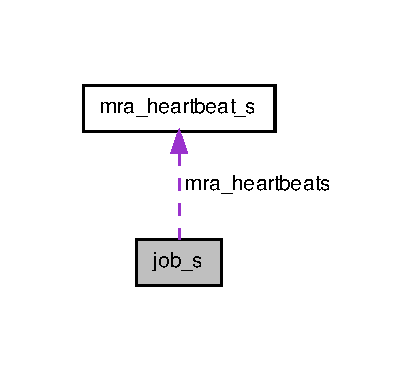
\includegraphics[width=199pt]{structjob__s__coll__graph}
\end{center}
\end{figure}
\subsection*{\-Data \-Fields}
\begin{DoxyCompactItemize}
\item 
int \hyperlink{structjob__s_ab8937d6bc68b0fc735d85461886a5d81}{finished}
\item 
int \hyperlink{structjob__s_a2121f93a58679fe228efdefe7bdcd1ba}{tasks\-\_\-pending} \mbox{[}2\mbox{]}
\item 
int $\ast$ \hyperlink{structjob__s_a511f43e33a73ddbda1ec080c2f972e33}{task\-\_\-instances} \mbox{[}2\mbox{]}
\item 
int $\ast$ \hyperlink{structjob__s_a25c05f7bc2c55b8626a947c42fbea207}{task\-\_\-status} \mbox{[}2\mbox{]}
\item 
msg\-\_\-task\-\_\-t $\ast$$\ast$ \hyperlink{structjob__s_a30c1a20fc86906cb521672940ff65c0f}{task\-\_\-list} \mbox{[}2\mbox{]}
\item 
size\-\_\-t $\ast$$\ast$ \hyperlink{structjob__s_aaf7015affb185128aab0ad5420310c74}{map\-\_\-output}
\item 
\hyperlink{common-mra_8h_a9a9d834f744f36f4e51ebf6c532e26bd}{mra\-\_\-heartbeat\-\_\-t} \hyperlink{structjob__s_a7e379eed44e91688e48a9ff5ff5a12c9}{mra\-\_\-heartbeats}
\end{DoxyCompactItemize}


\subsection{\-Field \-Documentation}
\hypertarget{structjob__s_ab8937d6bc68b0fc735d85461886a5d81}{\index{job\-\_\-s@{job\-\_\-s}!finished@{finished}}
\index{finished@{finished}!job_s@{job\-\_\-s}}
\subsubsection[{finished}]{\setlength{\rightskip}{0pt plus 5cm}int {\bf job\-\_\-s\-::finished}}}\label{structjob__s_ab8937d6bc68b0fc735d85461886a5d81}
\hypertarget{structjob__s_aaf7015affb185128aab0ad5420310c74}{\index{job\-\_\-s@{job\-\_\-s}!map\-\_\-output@{map\-\_\-output}}
\index{map\-\_\-output@{map\-\_\-output}!job_s@{job\-\_\-s}}
\subsubsection[{map\-\_\-output}]{\setlength{\rightskip}{0pt plus 5cm}size\-\_\-t$\ast$$\ast$ {\bf job\-\_\-s\-::map\-\_\-output}}}\label{structjob__s_aaf7015affb185128aab0ad5420310c74}
\hypertarget{structjob__s_a7e379eed44e91688e48a9ff5ff5a12c9}{\index{job\-\_\-s@{job\-\_\-s}!mra\-\_\-heartbeats@{mra\-\_\-heartbeats}}
\index{mra\-\_\-heartbeats@{mra\-\_\-heartbeats}!job_s@{job\-\_\-s}}
\subsubsection[{mra\-\_\-heartbeats}]{\setlength{\rightskip}{0pt plus 5cm}{\bf mra\-\_\-heartbeat\-\_\-t} {\bf job\-\_\-s\-::mra\-\_\-heartbeats}}}\label{structjob__s_a7e379eed44e91688e48a9ff5ff5a12c9}
\hypertarget{structjob__s_a511f43e33a73ddbda1ec080c2f972e33}{\index{job\-\_\-s@{job\-\_\-s}!task\-\_\-instances@{task\-\_\-instances}}
\index{task\-\_\-instances@{task\-\_\-instances}!job_s@{job\-\_\-s}}
\subsubsection[{task\-\_\-instances}]{\setlength{\rightskip}{0pt plus 5cm}int$\ast$ {\bf job\-\_\-s\-::task\-\_\-instances}\mbox{[}2\mbox{]}}}\label{structjob__s_a511f43e33a73ddbda1ec080c2f972e33}
\hypertarget{structjob__s_a30c1a20fc86906cb521672940ff65c0f}{\index{job\-\_\-s@{job\-\_\-s}!task\-\_\-list@{task\-\_\-list}}
\index{task\-\_\-list@{task\-\_\-list}!job_s@{job\-\_\-s}}
\subsubsection[{task\-\_\-list}]{\setlength{\rightskip}{0pt plus 5cm}msg\-\_\-task\-\_\-t$\ast$$\ast$ {\bf job\-\_\-s\-::task\-\_\-list}\mbox{[}2\mbox{]}}}\label{structjob__s_a30c1a20fc86906cb521672940ff65c0f}
\hypertarget{structjob__s_a25c05f7bc2c55b8626a947c42fbea207}{\index{job\-\_\-s@{job\-\_\-s}!task\-\_\-status@{task\-\_\-status}}
\index{task\-\_\-status@{task\-\_\-status}!job_s@{job\-\_\-s}}
\subsubsection[{task\-\_\-status}]{\setlength{\rightskip}{0pt plus 5cm}int$\ast$ {\bf job\-\_\-s\-::task\-\_\-status}\mbox{[}2\mbox{]}}}\label{structjob__s_a25c05f7bc2c55b8626a947c42fbea207}
\hypertarget{structjob__s_a2121f93a58679fe228efdefe7bdcd1ba}{\index{job\-\_\-s@{job\-\_\-s}!tasks\-\_\-pending@{tasks\-\_\-pending}}
\index{tasks\-\_\-pending@{tasks\-\_\-pending}!job_s@{job\-\_\-s}}
\subsubsection[{tasks\-\_\-pending}]{\setlength{\rightskip}{0pt plus 5cm}int {\bf job\-\_\-s\-::tasks\-\_\-pending}\mbox{[}2\mbox{]}}}\label{structjob__s_a2121f93a58679fe228efdefe7bdcd1ba}


\-The documentation for this struct was generated from the following file\-:\begin{DoxyCompactItemize}
\item 
include/\hyperlink{common-mra_8h}{common-\/mra.\-h}\end{DoxyCompactItemize}

\hypertarget{structmra__heartbeat__s}{\section{mra\-\_\-heartbeat\-\_\-s \-Struct \-Reference}
\label{structmra__heartbeat__s}\index{mra\-\_\-heartbeat\-\_\-s@{mra\-\_\-heartbeat\-\_\-s}}
}


\-Information sent by the workers with every heartbeat.  




{\ttfamily \#include $<$common\-\_\-mra.\-h$>$}

\subsection*{\-Data \-Fields}
\begin{DoxyCompactItemize}
\item 
int \hyperlink{structmra__heartbeat__s_a4807e7c902185697b22776045965e1a6}{slots\-\_\-av} \mbox{[}2\mbox{]}
\end{DoxyCompactItemize}


\subsection{\-Detailed \-Description}
\-Information sent by the workers with every heartbeat. 

\subsection{\-Field \-Documentation}
\hypertarget{structmra__heartbeat__s_a4807e7c902185697b22776045965e1a6}{\index{mra\-\_\-heartbeat\-\_\-s@{mra\-\_\-heartbeat\-\_\-s}!slots\-\_\-av@{slots\-\_\-av}}
\index{slots\-\_\-av@{slots\-\_\-av}!mra_heartbeat_s@{mra\-\_\-heartbeat\-\_\-s}}
\subsubsection[{slots\-\_\-av}]{\setlength{\rightskip}{0pt plus 5cm}int {\bf mra\-\_\-heartbeat\-\_\-s\-::slots\-\_\-av}\mbox{[}2\mbox{]}}}\label{structmra__heartbeat__s_a4807e7c902185697b22776045965e1a6}


\-The documentation for this struct was generated from the following file\-:\begin{DoxyCompactItemize}
\item 
include/\hyperlink{common__mra_8h}{common\-\_\-mra.\-h}\end{DoxyCompactItemize}

\hypertarget{structstats__s}{\section{stats\-\_\-s \-Struct \-Reference}
\label{structstats__s}\index{stats\-\_\-s@{stats\-\_\-s}}
}


{\ttfamily \#include $<$common-\/mra.\-h$>$}

\subsection*{\-Data \-Fields}
\begin{DoxyCompactItemize}
\item 
int \hyperlink{structstats__s_ac3b2752238687f8f231dc7ee3fb66126}{map\-\_\-local}
\item 
int \hyperlink{structstats__s_ae49231fe6e7f535421d0b0cc63af8324}{mra\-\_\-map\-\_\-remote}
\item 
int \hyperlink{structstats__s_a8928364ec78465521407e3978bb0256b}{map\-\_\-spec\-\_\-l}
\item 
int \hyperlink{structstats__s_aaa36a987438e3743fb4fddf2e3b766ac}{map\-\_\-spec\-\_\-r}
\item 
int \hyperlink{structstats__s_ac416c784bd8cc7f6ff36fc0424a3e3bc}{reduce\-\_\-normal}
\item 
int \hyperlink{structstats__s_a72a455323e2db452773d6e4d21fe8554}{reduce\-\_\-spec}
\end{DoxyCompactItemize}


\subsection{\-Field \-Documentation}
\hypertarget{structstats__s_ac3b2752238687f8f231dc7ee3fb66126}{\index{stats\-\_\-s@{stats\-\_\-s}!map\-\_\-local@{map\-\_\-local}}
\index{map\-\_\-local@{map\-\_\-local}!stats_s@{stats\-\_\-s}}
\subsubsection[{map\-\_\-local}]{\setlength{\rightskip}{0pt plus 5cm}int {\bf stats\-\_\-s\-::map\-\_\-local}}}\label{structstats__s_ac3b2752238687f8f231dc7ee3fb66126}
\hypertarget{structstats__s_a8928364ec78465521407e3978bb0256b}{\index{stats\-\_\-s@{stats\-\_\-s}!map\-\_\-spec\-\_\-l@{map\-\_\-spec\-\_\-l}}
\index{map\-\_\-spec\-\_\-l@{map\-\_\-spec\-\_\-l}!stats_s@{stats\-\_\-s}}
\subsubsection[{map\-\_\-spec\-\_\-l}]{\setlength{\rightskip}{0pt plus 5cm}int {\bf stats\-\_\-s\-::map\-\_\-spec\-\_\-l}}}\label{structstats__s_a8928364ec78465521407e3978bb0256b}
\hypertarget{structstats__s_aaa36a987438e3743fb4fddf2e3b766ac}{\index{stats\-\_\-s@{stats\-\_\-s}!map\-\_\-spec\-\_\-r@{map\-\_\-spec\-\_\-r}}
\index{map\-\_\-spec\-\_\-r@{map\-\_\-spec\-\_\-r}!stats_s@{stats\-\_\-s}}
\subsubsection[{map\-\_\-spec\-\_\-r}]{\setlength{\rightskip}{0pt plus 5cm}int {\bf stats\-\_\-s\-::map\-\_\-spec\-\_\-r}}}\label{structstats__s_aaa36a987438e3743fb4fddf2e3b766ac}
\hypertarget{structstats__s_ae49231fe6e7f535421d0b0cc63af8324}{\index{stats\-\_\-s@{stats\-\_\-s}!mra\-\_\-map\-\_\-remote@{mra\-\_\-map\-\_\-remote}}
\index{mra\-\_\-map\-\_\-remote@{mra\-\_\-map\-\_\-remote}!stats_s@{stats\-\_\-s}}
\subsubsection[{mra\-\_\-map\-\_\-remote}]{\setlength{\rightskip}{0pt plus 5cm}int {\bf stats\-\_\-s\-::mra\-\_\-map\-\_\-remote}}}\label{structstats__s_ae49231fe6e7f535421d0b0cc63af8324}
\hypertarget{structstats__s_ac416c784bd8cc7f6ff36fc0424a3e3bc}{\index{stats\-\_\-s@{stats\-\_\-s}!reduce\-\_\-normal@{reduce\-\_\-normal}}
\index{reduce\-\_\-normal@{reduce\-\_\-normal}!stats_s@{stats\-\_\-s}}
\subsubsection[{reduce\-\_\-normal}]{\setlength{\rightskip}{0pt plus 5cm}int {\bf stats\-\_\-s\-::reduce\-\_\-normal}}}\label{structstats__s_ac416c784bd8cc7f6ff36fc0424a3e3bc}
\hypertarget{structstats__s_a72a455323e2db452773d6e4d21fe8554}{\index{stats\-\_\-s@{stats\-\_\-s}!reduce\-\_\-spec@{reduce\-\_\-spec}}
\index{reduce\-\_\-spec@{reduce\-\_\-spec}!stats_s@{stats\-\_\-s}}
\subsubsection[{reduce\-\_\-spec}]{\setlength{\rightskip}{0pt plus 5cm}int {\bf stats\-\_\-s\-::reduce\-\_\-spec}}}\label{structstats__s_a72a455323e2db452773d6e4d21fe8554}


\-The documentation for this struct was generated from the following file\-:\begin{DoxyCompactItemize}
\item 
include/\hyperlink{common-mra_8h}{common-\/mra.\-h}\end{DoxyCompactItemize}

\hypertarget{structtask__info__s}{\section{task\-\_\-info\-\_\-s \-Struct \-Reference}
\label{structtask__info__s}\index{task\-\_\-info\-\_\-s@{task\-\_\-info\-\_\-s}}
}


\-Information sent as the task data.  




{\ttfamily \#include $<$common\-\_\-mra.\-h$>$}

\subsection*{\-Data \-Fields}
\begin{DoxyCompactItemize}
\item 
enum \hyperlink{mra_8h_afa14b6e068c0e0b8557777e16f2582f2}{phase\-\_\-e} \hyperlink{structtask__info__s_afa72d514e04545e1916981f970178902}{phase}
\item 
size\-\_\-t \hyperlink{structtask__info__s_a4974ced5dfb8d5d2ab72351cc12e1bb6}{id}
\item 
size\-\_\-t \hyperlink{structtask__info__s_a80e71f08fc31bfe88a8c546f0e8155d7}{src}
\item 
size\-\_\-t \hyperlink{structtask__info__s_a7b70c65e767769e2a42e6c5978c2c669}{wid}
\item 
int \hyperlink{structtask__info__s_abf5e8401c80afb200b761ed7207cfcea}{pid}
\item 
msg\-\_\-task\-\_\-t \hyperlink{structtask__info__s_a852100955a5ed323f31c670ef596787c}{task}
\item 
size\-\_\-t $\ast$ \hyperlink{structtask__info__s_a89d391613219da550d84283a89461bf4}{map\-\_\-output\-\_\-copied}
\item 
double \hyperlink{structtask__info__s_a3f07b243958c81aab30d87f2f8aa63c3}{shuffle\-\_\-mra\-\_\-end}
\end{DoxyCompactItemize}


\subsection{\-Detailed \-Description}
\-Information sent as the task data. 

\subsection{\-Field \-Documentation}
\hypertarget{structtask__info__s_a4974ced5dfb8d5d2ab72351cc12e1bb6}{\index{task\-\_\-info\-\_\-s@{task\-\_\-info\-\_\-s}!id@{id}}
\index{id@{id}!task_info_s@{task\-\_\-info\-\_\-s}}
\subsubsection[{id}]{\setlength{\rightskip}{0pt plus 5cm}size\-\_\-t {\bf task\-\_\-info\-\_\-s\-::id}}}\label{structtask__info__s_a4974ced5dfb8d5d2ab72351cc12e1bb6}
\hypertarget{structtask__info__s_a89d391613219da550d84283a89461bf4}{\index{task\-\_\-info\-\_\-s@{task\-\_\-info\-\_\-s}!map\-\_\-output\-\_\-copied@{map\-\_\-output\-\_\-copied}}
\index{map\-\_\-output\-\_\-copied@{map\-\_\-output\-\_\-copied}!task_info_s@{task\-\_\-info\-\_\-s}}
\subsubsection[{map\-\_\-output\-\_\-copied}]{\setlength{\rightskip}{0pt plus 5cm}size\-\_\-t$\ast$ {\bf task\-\_\-info\-\_\-s\-::map\-\_\-output\-\_\-copied}}}\label{structtask__info__s_a89d391613219da550d84283a89461bf4}
\hypertarget{structtask__info__s_afa72d514e04545e1916981f970178902}{\index{task\-\_\-info\-\_\-s@{task\-\_\-info\-\_\-s}!phase@{phase}}
\index{phase@{phase}!task_info_s@{task\-\_\-info\-\_\-s}}
\subsubsection[{phase}]{\setlength{\rightskip}{0pt plus 5cm}enum {\bf phase\-\_\-e} {\bf task\-\_\-info\-\_\-s\-::phase}}}\label{structtask__info__s_afa72d514e04545e1916981f970178902}
\hypertarget{structtask__info__s_abf5e8401c80afb200b761ed7207cfcea}{\index{task\-\_\-info\-\_\-s@{task\-\_\-info\-\_\-s}!pid@{pid}}
\index{pid@{pid}!task_info_s@{task\-\_\-info\-\_\-s}}
\subsubsection[{pid}]{\setlength{\rightskip}{0pt plus 5cm}int {\bf task\-\_\-info\-\_\-s\-::pid}}}\label{structtask__info__s_abf5e8401c80afb200b761ed7207cfcea}
\hypertarget{structtask__info__s_a3f07b243958c81aab30d87f2f8aa63c3}{\index{task\-\_\-info\-\_\-s@{task\-\_\-info\-\_\-s}!shuffle\-\_\-mra\-\_\-end@{shuffle\-\_\-mra\-\_\-end}}
\index{shuffle\-\_\-mra\-\_\-end@{shuffle\-\_\-mra\-\_\-end}!task_info_s@{task\-\_\-info\-\_\-s}}
\subsubsection[{shuffle\-\_\-mra\-\_\-end}]{\setlength{\rightskip}{0pt plus 5cm}double {\bf task\-\_\-info\-\_\-s\-::shuffle\-\_\-mra\-\_\-end}}}\label{structtask__info__s_a3f07b243958c81aab30d87f2f8aa63c3}
\hypertarget{structtask__info__s_a80e71f08fc31bfe88a8c546f0e8155d7}{\index{task\-\_\-info\-\_\-s@{task\-\_\-info\-\_\-s}!src@{src}}
\index{src@{src}!task_info_s@{task\-\_\-info\-\_\-s}}
\subsubsection[{src}]{\setlength{\rightskip}{0pt plus 5cm}size\-\_\-t {\bf task\-\_\-info\-\_\-s\-::src}}}\label{structtask__info__s_a80e71f08fc31bfe88a8c546f0e8155d7}
\hypertarget{structtask__info__s_a852100955a5ed323f31c670ef596787c}{\index{task\-\_\-info\-\_\-s@{task\-\_\-info\-\_\-s}!task@{task}}
\index{task@{task}!task_info_s@{task\-\_\-info\-\_\-s}}
\subsubsection[{task}]{\setlength{\rightskip}{0pt plus 5cm}msg\-\_\-task\-\_\-t {\bf task\-\_\-info\-\_\-s\-::task}}}\label{structtask__info__s_a852100955a5ed323f31c670ef596787c}
\hypertarget{structtask__info__s_a7b70c65e767769e2a42e6c5978c2c669}{\index{task\-\_\-info\-\_\-s@{task\-\_\-info\-\_\-s}!wid@{wid}}
\index{wid@{wid}!task_info_s@{task\-\_\-info\-\_\-s}}
\subsubsection[{wid}]{\setlength{\rightskip}{0pt plus 5cm}size\-\_\-t {\bf task\-\_\-info\-\_\-s\-::wid}}}\label{structtask__info__s_a7b70c65e767769e2a42e6c5978c2c669}


\-The documentation for this struct was generated from the following file\-:\begin{DoxyCompactItemize}
\item 
include/\hyperlink{common__mra_8h}{common\-\_\-mra.\-h}\end{DoxyCompactItemize}

\hypertarget{structuser__s}{\section{user\-\_\-s \-Struct \-Reference}
\label{structuser__s}\index{user\-\_\-s@{user\-\_\-s}}
}


{\ttfamily \#include $<$common-\/mra.\-h$>$}

\subsection*{\-Data \-Fields}
\begin{DoxyCompactItemize}
\item 
double($\ast$ \hyperlink{structuser__s_aa32af3ea6ee92e53a04476911d65f2c1}{task\-\_\-mra\-\_\-cost\-\_\-f} )(enum \hyperlink{mra_8h_afa14b6e068c0e0b8557777e16f2582f2}{phase\-\_\-e} phase, size\-\_\-t tid, size\-\_\-t wid)
\item 
void($\ast$ \hyperlink{structuser__s_a832e7d465f899e75aa7fe1d72987c5d2}{mra\-\_\-dfs\-\_\-f} )(char $\ast$$\ast$mra\-\_\-dfs\-\_\-matrix, size\-\_\-t chunks, size\-\_\-t workers\-\_\-mra, int replicas)
\item 
int($\ast$ \hyperlink{structuser__s_ab9a47b1668a675fb95ca6489d1da13a7}{map\-\_\-mra\-\_\-output\-\_\-f} )(size\-\_\-t mid, size\-\_\-t rid)
\end{DoxyCompactItemize}


\subsection{\-Field \-Documentation}
\hypertarget{structuser__s_ab9a47b1668a675fb95ca6489d1da13a7}{\index{user\-\_\-s@{user\-\_\-s}!map\-\_\-mra\-\_\-output\-\_\-f@{map\-\_\-mra\-\_\-output\-\_\-f}}
\index{map\-\_\-mra\-\_\-output\-\_\-f@{map\-\_\-mra\-\_\-output\-\_\-f}!user_s@{user\-\_\-s}}
\subsubsection[{map\-\_\-mra\-\_\-output\-\_\-f}]{\setlength{\rightskip}{0pt plus 5cm}int($\ast$ {\bf user\-\_\-s\-::map\-\_\-mra\-\_\-output\-\_\-f})(size\-\_\-t mid, size\-\_\-t rid)}}\label{structuser__s_ab9a47b1668a675fb95ca6489d1da13a7}
\hypertarget{structuser__s_a832e7d465f899e75aa7fe1d72987c5d2}{\index{user\-\_\-s@{user\-\_\-s}!mra\-\_\-dfs\-\_\-f@{mra\-\_\-dfs\-\_\-f}}
\index{mra\-\_\-dfs\-\_\-f@{mra\-\_\-dfs\-\_\-f}!user_s@{user\-\_\-s}}
\subsubsection[{mra\-\_\-dfs\-\_\-f}]{\setlength{\rightskip}{0pt plus 5cm}void($\ast$ {\bf user\-\_\-s\-::mra\-\_\-dfs\-\_\-f})(char $\ast$$\ast$mra\-\_\-dfs\-\_\-matrix, size\-\_\-t chunks, size\-\_\-t workers\-\_\-mra, int replicas)}}\label{structuser__s_a832e7d465f899e75aa7fe1d72987c5d2}
\hypertarget{structuser__s_aa32af3ea6ee92e53a04476911d65f2c1}{\index{user\-\_\-s@{user\-\_\-s}!task\-\_\-mra\-\_\-cost\-\_\-f@{task\-\_\-mra\-\_\-cost\-\_\-f}}
\index{task\-\_\-mra\-\_\-cost\-\_\-f@{task\-\_\-mra\-\_\-cost\-\_\-f}!user_s@{user\-\_\-s}}
\subsubsection[{task\-\_\-mra\-\_\-cost\-\_\-f}]{\setlength{\rightskip}{0pt plus 5cm}double($\ast$ {\bf user\-\_\-s\-::task\-\_\-mra\-\_\-cost\-\_\-f})(enum {\bf phase\-\_\-e} phase, size\-\_\-t tid, size\-\_\-t wid)}}\label{structuser__s_aa32af3ea6ee92e53a04476911d65f2c1}


\-The documentation for this struct was generated from the following file\-:\begin{DoxyCompactItemize}
\item 
include/\hyperlink{common-mra_8h}{common-\/mra.\-h}\end{DoxyCompactItemize}

\hypertarget{structw__info__s}{\section{w\-\_\-info\-\_\-s \-Struct \-Reference}
\label{structw__info__s}\index{w\-\_\-info\-\_\-s@{w\-\_\-info\-\_\-s}}
}


{\ttfamily \#include $<$worker-\/mra.\-h$>$}

\subsection*{\-Data \-Fields}
\begin{DoxyCompactItemize}
\item 
size\-\_\-t \hyperlink{structw__info__s_ae293128296d6f73011e64ebbd840cb0c}{wid}
\end{DoxyCompactItemize}


\subsection{\-Field \-Documentation}
\hypertarget{structw__info__s_ae293128296d6f73011e64ebbd840cb0c}{\index{w\-\_\-info\-\_\-s@{w\-\_\-info\-\_\-s}!wid@{wid}}
\index{wid@{wid}!w_info_s@{w\-\_\-info\-\_\-s}}
\subsubsection[{wid}]{\setlength{\rightskip}{0pt plus 5cm}size\-\_\-t {\bf w\-\_\-info\-\_\-s\-::wid}}}\label{structw__info__s_ae293128296d6f73011e64ebbd840cb0c}


\-The documentation for this struct was generated from the following file\-:\begin{DoxyCompactItemize}
\item 
include/\hyperlink{worker-mra_8h}{worker-\/mra.\-h}\end{DoxyCompactItemize}

\chapter{\-File \-Documentation}
\hypertarget{hello_8c}{\section{examples/hello.c \-File \-Reference}
\label{hello_8c}\index{examples/hello.\-c@{examples/hello.\-c}}
}
{\ttfamily \#include \char`\"{}common-\/mra.\-h\char`\"{}}\*
{\ttfamily \#include $<$mra.\-h$>$}\*
\-Include dependency graph for hello.\-c\-:\nopagebreak
\begin{figure}[H]
\begin{center}
\leavevmode
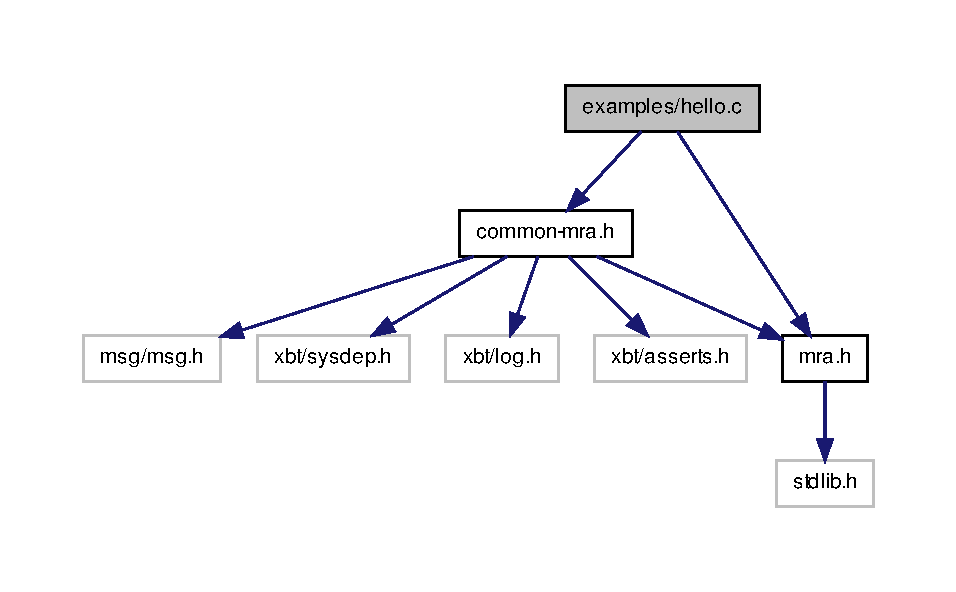
\includegraphics[width=350pt]{hello_8c__incl}
\end{center}
\end{figure}
\subsection*{\-Functions}
\begin{DoxyCompactItemize}
\item 
static void \hyperlink{hello_8c_a88af1c2716456427567c196ae8d35387}{read\-\_\-mra\-\_\-config\-\_\-file} (const char $\ast$file\-\_\-name)
\item 
int \hyperlink{hello_8c_a7bab67503d755ceaddde21aed4dc1f7b}{mra\-\_\-map\-\_\-mra\-\_\-output\-\_\-function} (size\-\_\-t mid, size\-\_\-t rid)
\item 
double \hyperlink{hello_8c_aea053eb2bc9377f4966d604dd0450485}{mra\-\_\-task\-\_\-mra\-\_\-cost\-\_\-function} (enum \hyperlink{mra_8h_afa14b6e068c0e0b8557777e16f2582f2}{phase\-\_\-e} phase, size\-\_\-t tid, size\-\_\-t wid)
\item 
int \hyperlink{hello_8c_a0ddf1224851353fc92bfbff6f499fa97}{main} (int argc, char $\ast$argv\mbox{[}$\,$\mbox{]})
\end{DoxyCompactItemize}


\subsection{\-Function \-Documentation}
\hypertarget{hello_8c_a0ddf1224851353fc92bfbff6f499fa97}{\index{hello.\-c@{hello.\-c}!main@{main}}
\index{main@{main}!hello.c@{hello.\-c}}
\subsubsection[{main}]{\setlength{\rightskip}{0pt plus 5cm}int {\bf main} (
\begin{DoxyParamCaption}
\item[{int}]{argc, }
\item[{char $\ast$}]{argv\mbox{[}$\,$\mbox{]}}
\end{DoxyParamCaption}
)}}\label{hello_8c_a0ddf1224851353fc92bfbff6f499fa97}


\-Here is the call graph for this function\-:\nopagebreak
\begin{figure}[H]
\begin{center}
\leavevmode
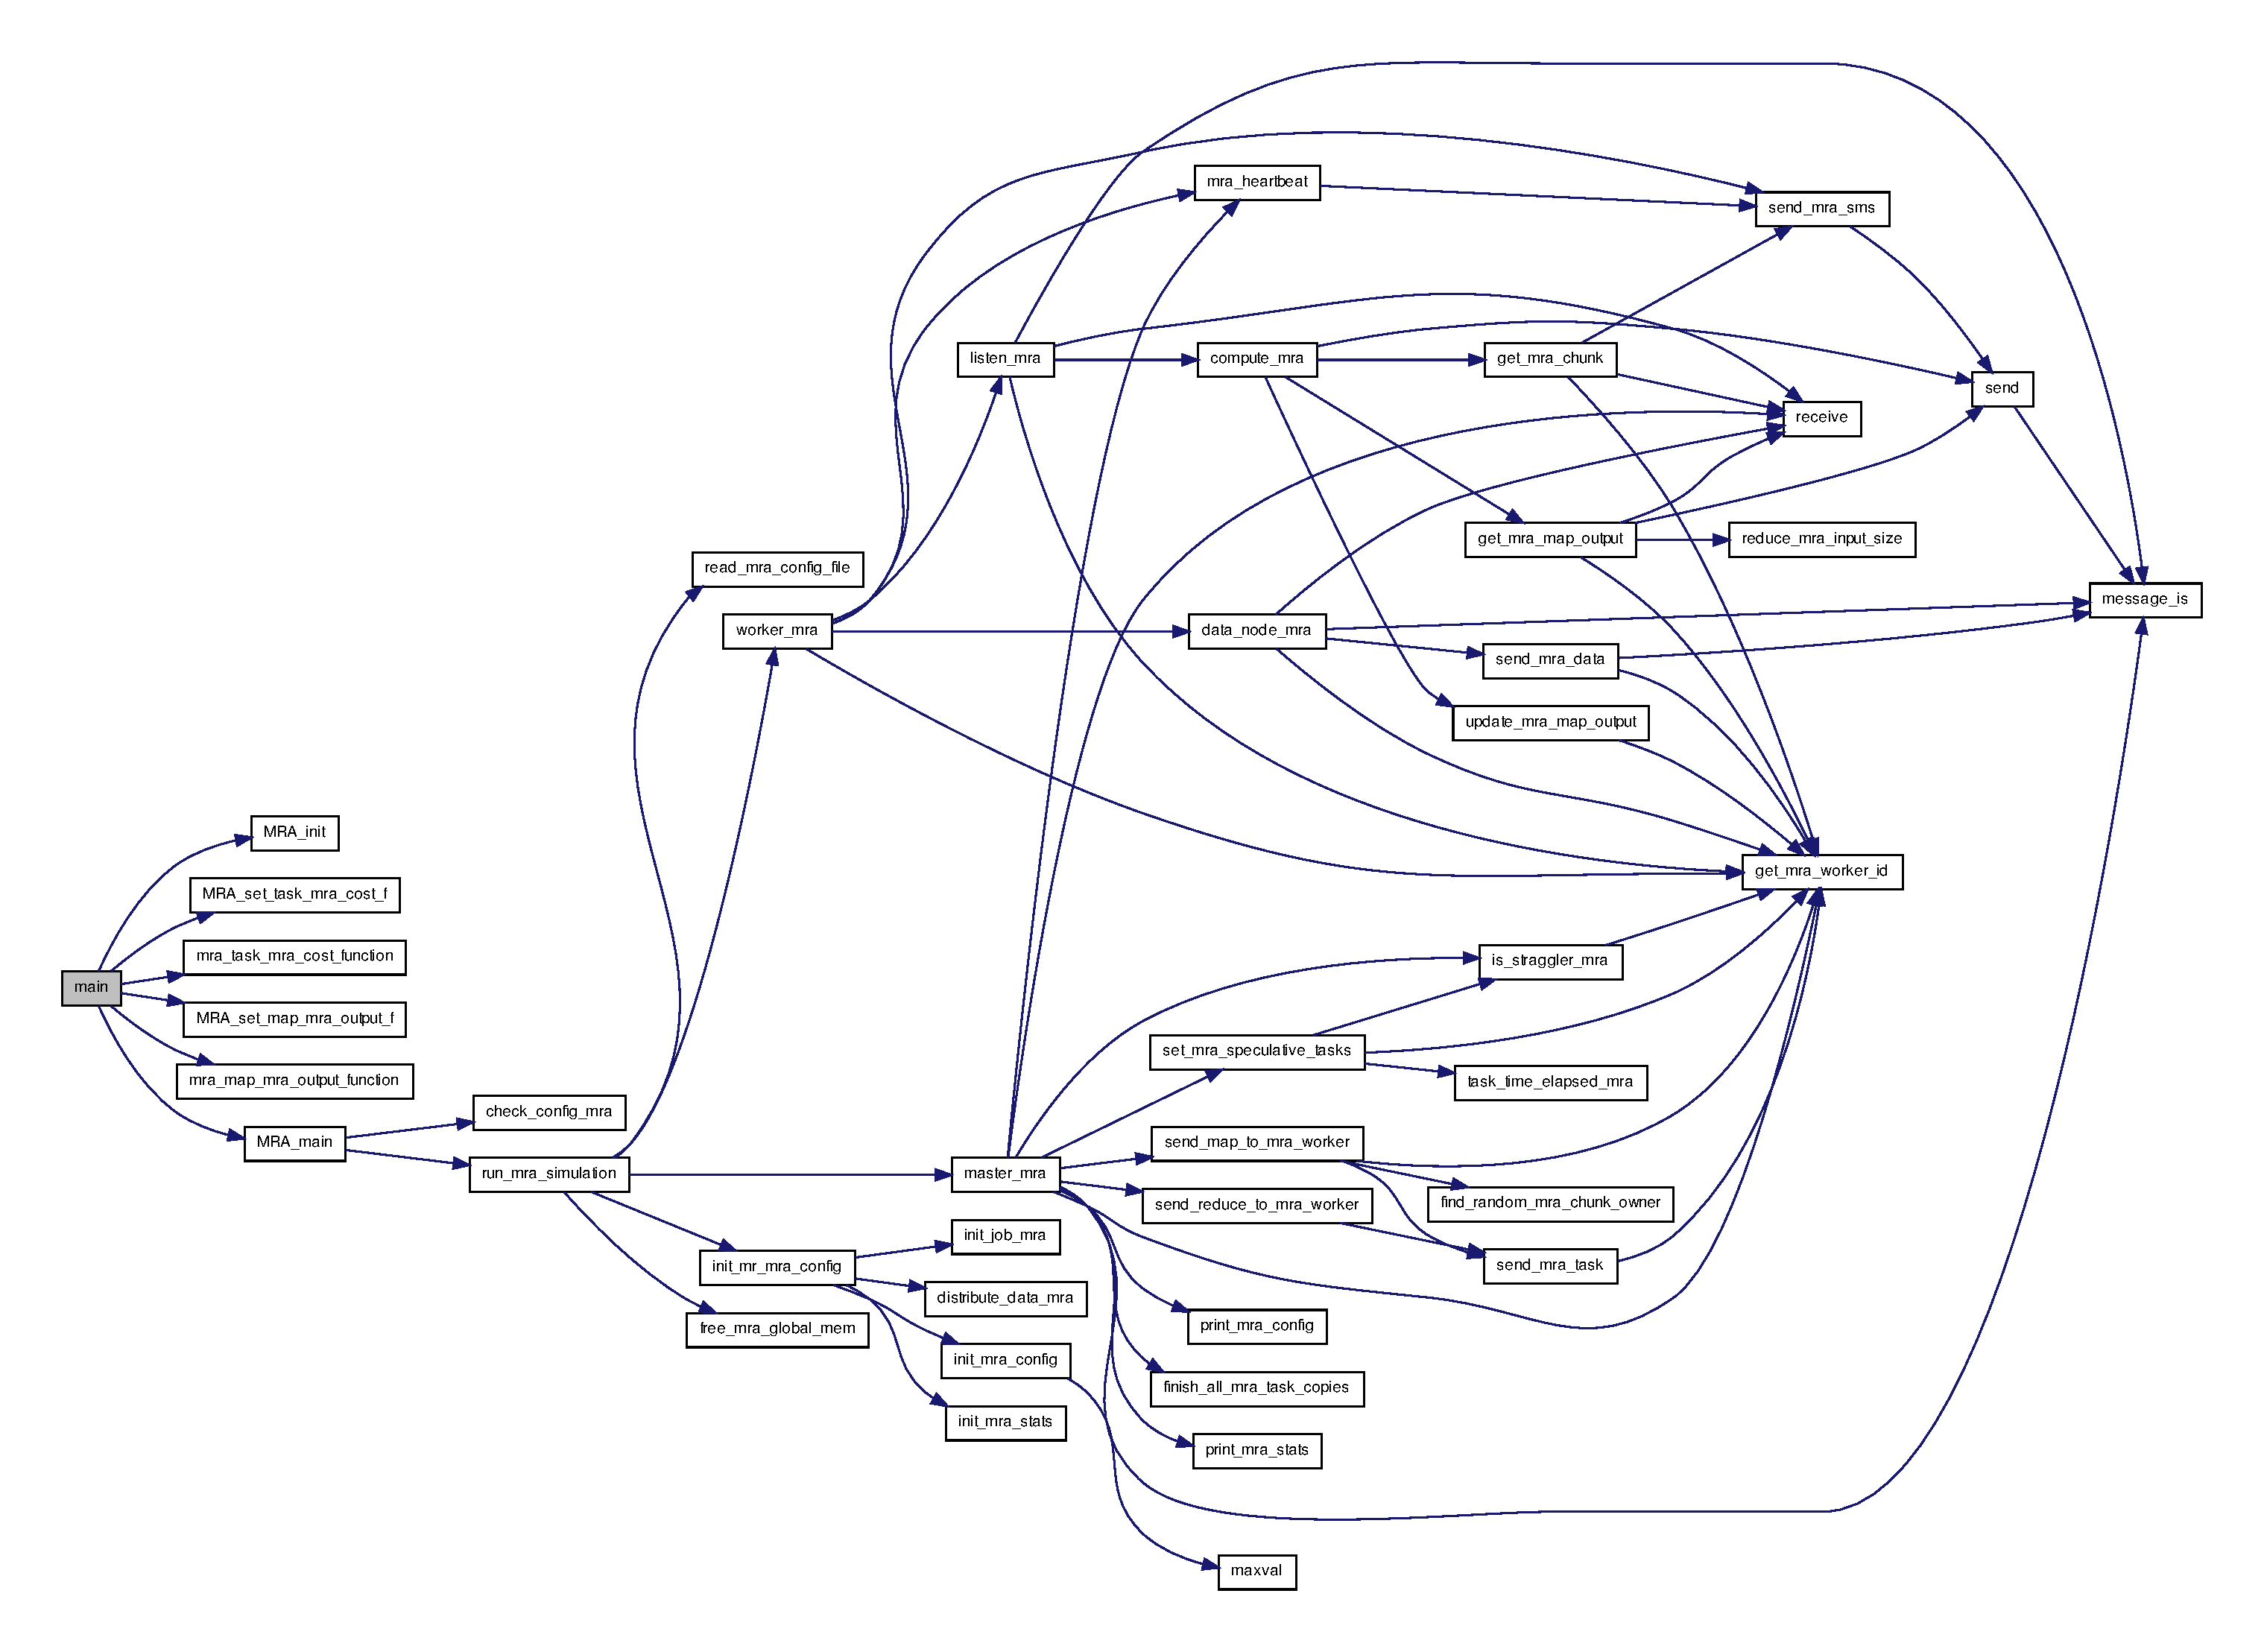
\includegraphics[width=350pt]{hello_8c_a0ddf1224851353fc92bfbff6f499fa97_cgraph}
\end{center}
\end{figure}


\hypertarget{hello_8c_a7bab67503d755ceaddde21aed4dc1f7b}{\index{hello.\-c@{hello.\-c}!mra\-\_\-map\-\_\-mra\-\_\-output\-\_\-function@{mra\-\_\-map\-\_\-mra\-\_\-output\-\_\-function}}
\index{mra\-\_\-map\-\_\-mra\-\_\-output\-\_\-function@{mra\-\_\-map\-\_\-mra\-\_\-output\-\_\-function}!hello.c@{hello.\-c}}
\subsubsection[{mra\-\_\-map\-\_\-mra\-\_\-output\-\_\-function}]{\setlength{\rightskip}{0pt plus 5cm}int {\bf mra\-\_\-map\-\_\-mra\-\_\-output\-\_\-function} (
\begin{DoxyParamCaption}
\item[{size\-\_\-t}]{mid, }
\item[{size\-\_\-t}]{rid}
\end{DoxyParamCaption}
)}}\label{hello_8c_a7bab67503d755ceaddde21aed4dc1f7b}
\-User function that indicates the amount of bytes that a map task will emit to a reduce task.


\begin{DoxyParams}{\-Parameters}
{\em mid} & \-The \-I\-D of the map task. \\
\hline
{\em rid} & \-The \-I\-D of the reduce task. \\
\hline
\end{DoxyParams}
\begin{DoxyReturn}{\-Returns}
\-The amount of data emitted (in bytes). 
\end{DoxyReturn}


\-Here is the caller graph for this function\-:\nopagebreak
\begin{figure}[H]
\begin{center}
\leavevmode
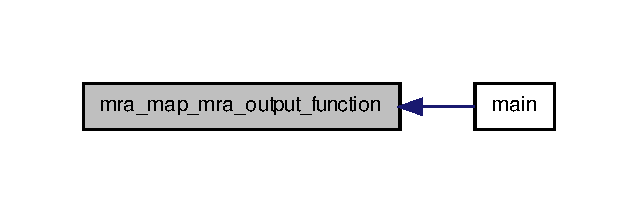
\includegraphics[width=306pt]{hello_8c_a7bab67503d755ceaddde21aed4dc1f7b_icgraph}
\end{center}
\end{figure}


\hypertarget{hello_8c_aea053eb2bc9377f4966d604dd0450485}{\index{hello.\-c@{hello.\-c}!mra\-\_\-task\-\_\-mra\-\_\-cost\-\_\-function@{mra\-\_\-task\-\_\-mra\-\_\-cost\-\_\-function}}
\index{mra\-\_\-task\-\_\-mra\-\_\-cost\-\_\-function@{mra\-\_\-task\-\_\-mra\-\_\-cost\-\_\-function}!hello.c@{hello.\-c}}
\subsubsection[{mra\-\_\-task\-\_\-mra\-\_\-cost\-\_\-function}]{\setlength{\rightskip}{0pt plus 5cm}double {\bf mra\-\_\-task\-\_\-mra\-\_\-cost\-\_\-function} (
\begin{DoxyParamCaption}
\item[{enum {\bf phase\-\_\-e}}]{phase, }
\item[{size\-\_\-t}]{tid, }
\item[{size\-\_\-t}]{wid}
\end{DoxyParamCaption}
)}}\label{hello_8c_aea053eb2bc9377f4966d604dd0450485}
\-User function that indicates the cost of a task.


\begin{DoxyParams}{\-Parameters}
{\em phase} & \-The execution phase. \\
\hline
{\em tid} & \-The \-I\-D of the task. \\
\hline
{\em wid} & \-The \-I\-D of the worker that received the task. \\
\hline
\end{DoxyParams}
\begin{DoxyReturn}{\-Returns}
\-The task cost in \-F\-L\-O\-Ps. 
\end{DoxyReturn}


\-Here is the caller graph for this function\-:\nopagebreak
\begin{figure}[H]
\begin{center}
\leavevmode
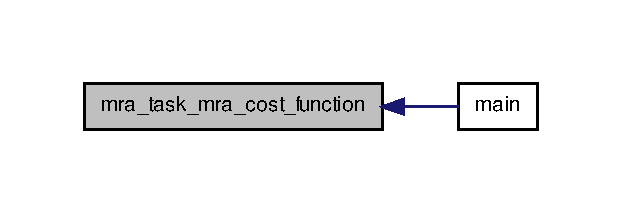
\includegraphics[width=298pt]{hello_8c_aea053eb2bc9377f4966d604dd0450485_icgraph}
\end{center}
\end{figure}


\hypertarget{hello_8c_a88af1c2716456427567c196ae8d35387}{\index{hello.\-c@{hello.\-c}!read\-\_\-mra\-\_\-config\-\_\-file@{read\-\_\-mra\-\_\-config\-\_\-file}}
\index{read\-\_\-mra\-\_\-config\-\_\-file@{read\-\_\-mra\-\_\-config\-\_\-file}!hello.c@{hello.\-c}}
\subsubsection[{read\-\_\-mra\-\_\-config\-\_\-file}]{\setlength{\rightskip}{0pt plus 5cm}static void {\bf read\-\_\-mra\-\_\-config\-\_\-file} (
\begin{DoxyParamCaption}
\item[{const char $\ast$}]{file\-\_\-name}
\end{DoxyParamCaption}
)\hspace{0.3cm}{\ttfamily  \mbox{[}static\mbox{]}}}}\label{hello_8c_a88af1c2716456427567c196ae8d35387}

\hypertarget{common-mra_8h}{\section{include/common-\/mra.h \-File \-Reference}
\label{common-mra_8h}\index{include/common-\/mra.\-h@{include/common-\/mra.\-h}}
}
{\ttfamily \#include $<$msg/msg.\-h$>$}\*
{\ttfamily \#include $<$xbt/sysdep.\-h$>$}\*
{\ttfamily \#include $<$xbt/log.\-h$>$}\*
{\ttfamily \#include $<$xbt/asserts.\-h$>$}\*
{\ttfamily \#include \char`\"{}mra.\-h\char`\"{}}\*
\-Include dependency graph for common-\/mra.h\-:\nopagebreak
\begin{figure}[H]
\begin{center}
\leavevmode
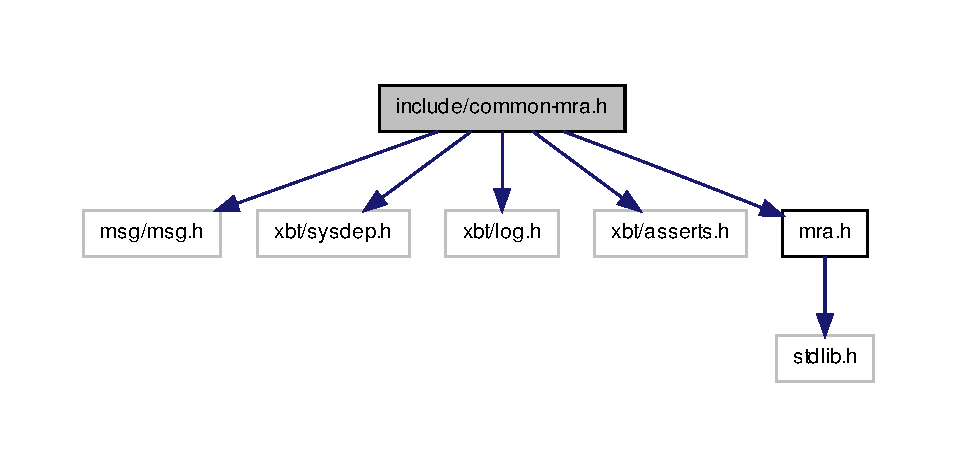
\includegraphics[width=350pt]{common-mra_8h__incl}
\end{center}
\end{figure}
\-This graph shows which files directly or indirectly include this file\-:\nopagebreak
\begin{figure}[H]
\begin{center}
\leavevmode
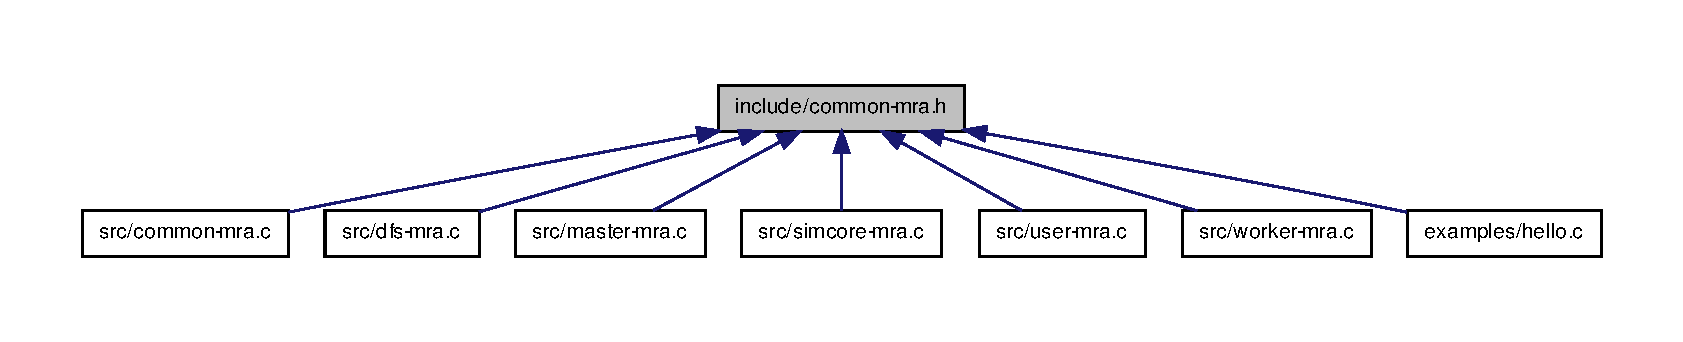
\includegraphics[width=350pt]{common-mra_8h__dep__incl}
\end{center}
\end{figure}
\subsection*{\-Data \-Structures}
\begin{DoxyCompactItemize}
\item 
struct \hyperlink{structmra__heartbeat__s}{mra\-\_\-heartbeat\-\_\-s}
\begin{DoxyCompactList}\small\item\em \-Information sent by the workers with every heartbeat. \end{DoxyCompactList}\item 
struct \hyperlink{structconfig__s}{config\-\_\-s}
\item 
struct \hyperlink{structjob__s}{job\-\_\-s}
\item 
struct \hyperlink{structtask__info__s}{task\-\_\-info\-\_\-s}
\begin{DoxyCompactList}\small\item\em \-Information sent as the task data. \end{DoxyCompactList}\item 
struct \hyperlink{structstats__s}{stats\-\_\-s}
\item 
struct \hyperlink{structuser__s}{user\-\_\-s}
\end{DoxyCompactItemize}
\subsection*{\-Defines}
\begin{DoxyCompactItemize}
\item 
\#define \hyperlink{common-mra_8h_a85026a76b45b05d1b98bb9a1d1ea5385}{\-M\-R\-A\-\_\-\-H\-E\-A\-R\-T\-B\-E\-A\-T\-\_\-\-M\-I\-N\-\_\-\-I\-N\-T\-E\-R\-V\-A\-L}~3
\item 
\#define \hyperlink{common-mra_8h_a2f68e94ff27ef3f63e98127818653e8f}{\-M\-R\-A\-\_\-\-H\-E\-A\-R\-T\-B\-E\-A\-T\-\_\-\-T\-I\-M\-E\-O\-U\-T}~600
\item 
\#define \hyperlink{common-mra_8h_ae17048f0a7244495add2d7bff7575b46}{\-S\-M\-S\-\_\-\-G\-E\-T\-\_\-\-M\-R\-A\-\_\-\-C\-H\-U\-N\-K}~\char`\"{}\-S\-M\-S-\/\-G\-C\char`\"{}
\item 
\#define \hyperlink{common-mra_8h_a82851de4a0b4080ee2fc4912bd5016c1}{\-S\-M\-S\-\_\-\-G\-E\-T\-\_\-\-I\-N\-T\-E\-R\-\_\-\-P\-A\-I\-R\-S}~\char`\"{}\-S\-M\-S-\/\-G\-I\-P\char`\"{}
\item 
\#define \hyperlink{common-mra_8h_aebb6b4972f6981a2c42945cc316fe2b5}{\-S\-M\-S\-\_\-\-M\-R\-A\-\_\-\-H\-E\-A\-R\-T\-B\-E\-A\-T}~\char`\"{}\-S\-M\-S-\/\-H\-B\char`\"{}
\item 
\#define \hyperlink{common-mra_8h_ae4152c1438f315591b56474d71caf421}{\-S\-M\-S\-\_\-\-T\-A\-S\-K}~\char`\"{}\-S\-M\-S-\/\-T\char`\"{}
\item 
\#define \hyperlink{common-mra_8h_a9872fc42f34693ee8407d6cee43765ac}{\-S\-M\-S\-\_\-\-T\-A\-S\-K\-\_\-\-D\-O\-N\-E}~\char`\"{}\-S\-M\-S-\/\-T\-D\char`\"{}
\item 
\#define \hyperlink{common-mra_8h_a441ebd93e24154f16983c901b282ebff}{\-S\-M\-S\-\_\-\-F\-I\-N\-I\-S\-H}~\char`\"{}\-S\-M\-S-\/\-F\char`\"{}
\item 
\#define \hyperlink{common-mra_8h_a655c84af1b0034986ff56e12e84f983d}{\-N\-O\-N\-E}~(-\/1)
\item 
\#define \hyperlink{common-mra_8h_a3a11044774f43ab067a966d654bc1fa8}{\-M\-A\-X\-\_\-\-S\-P\-E\-C\-U\-L\-A\-T\-I\-V\-E\-\_\-\-C\-O\-P\-I\-E\-S}~3
\item 
\#define \hyperlink{common-mra_8h_afaa0d742cbc433ed6d7dbb10dfd94670}{\-M\-A\-I\-L\-B\-O\-X\-\_\-\-A\-L\-I\-A\-S\-\_\-\-S\-I\-Z\-E}~256
\item 
\#define \hyperlink{common-mra_8h_a7648dbffbb9dd848a40b7c76cf5e4223}{\-M\-A\-S\-T\-E\-R\-\_\-\-M\-R\-A\-\_\-\-M\-A\-I\-L\-B\-O\-X}~\char`\"{}\-M\-A\-S\-T\-E\-R\-\_\-\-M\-R\-A\char`\"{}
\item 
\#define \hyperlink{common-mra_8h_a03ecfabdf95bb7456f21bcd120c76665}{\-D\-A\-T\-A\-N\-O\-D\-E\-\_\-\-M\-R\-A\-\_\-\-M\-A\-I\-L\-B\-O\-X}~\char`\"{}\%zu\-:\-D\-N\char`\"{}
\item 
\#define \hyperlink{common-mra_8h_a1366ac09f7a23b1235da07586d163ebe}{\-T\-A\-S\-K\-T\-R\-A\-C\-K\-E\-R\-\_\-\-M\-R\-A\-\_\-\-M\-A\-I\-L\-B\-O\-X}~\char`\"{}\%zu\-:\-T\-T\char`\"{}
\item 
\#define \hyperlink{common-mra_8h_ae559bdca40b1742557e7cebb210c8959}{\-T\-A\-S\-K\-\_\-\-M\-R\-A\-\_\-\-M\-A\-I\-L\-B\-O\-X}~\char`\"{}\%zu\-:\%d\char`\"{}
\end{DoxyCompactItemize}
\subsection*{\-Typedefs}
\begin{DoxyCompactItemize}
\item 
typedef struct \hyperlink{structmra__heartbeat__s}{mra\-\_\-heartbeat\-\_\-s} $\ast$ \hyperlink{common-mra_8h_a9a9d834f744f36f4e51ebf6c532e26bd}{mra\-\_\-heartbeat\-\_\-t}
\item 
typedef struct \hyperlink{structtask__info__s}{task\-\_\-info\-\_\-s} $\ast$ \hyperlink{common-mra_8h_a54f41524090023e9b283ecbef8b955d6}{mra\-\_\-task\-\_\-info\-\_\-t}
\end{DoxyCompactItemize}
\subsection*{\-Enumerations}
\begin{DoxyCompactItemize}
\item 
enum \hyperlink{common-mra_8h_aadf6e8ce08a315d3a320b05b2bcf27c7}{task\-\_\-status\-\_\-e} \{ \hyperlink{common-mra_8h_aadf6e8ce08a315d3a320b05b2bcf27c7a107af46c195ca17124951f9da9e4516e}{\-T\-\_\-\-S\-T\-A\-T\-U\-S\-\_\-\-M\-R\-A\-\_\-\-P\-E\-N\-D\-I\-N\-G}, 
\hyperlink{common-mra_8h_aadf6e8ce08a315d3a320b05b2bcf27c7a834ab8fd9011e98aadb58a05c2bcca7a}{\-T\-\_\-\-S\-T\-A\-T\-U\-S\-\_\-\-M\-R\-A\-\_\-\-T\-I\-P}, 
\hyperlink{common-mra_8h_aadf6e8ce08a315d3a320b05b2bcf27c7aad2c0fd8c428d4848bcbfe0e338bed95}{\-T\-\_\-\-S\-T\-A\-T\-U\-S\-\_\-\-M\-R\-A\-\_\-\-T\-I\-P\-\_\-\-S\-L\-O\-W}, 
\hyperlink{common-mra_8h_aadf6e8ce08a315d3a320b05b2bcf27c7a51f9b001d2b46f2aa6399622d2277520}{\-T\-\_\-\-S\-T\-A\-T\-U\-S\-\_\-\-M\-R\-A\-\_\-\-D\-O\-N\-E}
 \}
\begin{DoxyCompactList}\small\item\em \-Possible task status. \end{DoxyCompactList}\end{DoxyCompactItemize}
\subsection*{\-Functions}
\begin{DoxyCompactItemize}
\item 
msg\-\_\-error\-\_\-t \hyperlink{common-mra_8h_a385b12669d8faf7b5cdb54c1ae597e1c}{send} (const char $\ast$str, double cpu, double net, void $\ast$data, const char $\ast$mailbox)
\begin{DoxyCompactList}\small\item\em \-Send a message/task. \end{DoxyCompactList}\item 
msg\-\_\-error\-\_\-t \hyperlink{common-mra_8h_a305ac8e3389f94106990aa3c52c91416}{send\-\_\-mra\-\_\-sms} (const char $\ast$str, const char $\ast$mailbox)
\begin{DoxyCompactList}\small\item\em \-Send a short message, of size zero. \end{DoxyCompactList}\item 
msg\-\_\-error\-\_\-t \hyperlink{common-mra_8h_a6fc60933b9eabe64a880f68eba3131cc}{receive} (msg\-\_\-task\-\_\-t $\ast$msg, const char $\ast$mailbox)
\begin{DoxyCompactList}\small\item\em \-Receive a message/task from a mailbox. \end{DoxyCompactList}\item 
int \hyperlink{common-mra_8h_ad37a02c988c597622a346cb5293243fb}{message\-\_\-is} (msg\-\_\-task\-\_\-t msg, const char $\ast$str)
\begin{DoxyCompactList}\small\item\em \-Compare the message from a task with a string. \end{DoxyCompactList}\item 
int \hyperlink{common-mra_8h_a411d5133ab6881d40ef4cb44a7a47428}{maxval} (int a, int b)
\begin{DoxyCompactList}\small\item\em \-Return the maximum of two values. \end{DoxyCompactList}\item 
size\-\_\-t \hyperlink{common-mra_8h_a1df0d355a0754a40a7697437294d8431}{map\-\_\-mra\-\_\-output\-\_\-size} (size\-\_\-t mid)
\begin{DoxyCompactList}\small\item\em \-Return the output size of a map task. \end{DoxyCompactList}\item 
size\-\_\-t \hyperlink{common-mra_8h_a8205e98d4874b7e31f138d5016ad1eba}{reduce\-\_\-mra\-\_\-input\-\_\-size} (size\-\_\-t rid)
\begin{DoxyCompactList}\small\item\em \-Return the input size of a reduce task. \end{DoxyCompactList}\end{DoxyCompactItemize}
\subsection*{\-Variables}
\begin{DoxyCompactItemize}
\item 
int $\ast$ \hyperlink{common-mra_8h_a25cc609dae2875ebd3e01dec54626409}{dist\-\_\-bruta}
\begin{DoxyCompactList}\small\item\em \-Initialize dist\-\_\-bruta, task\-\_\-exec, avg\-\_\-task\-\_\-exec. \end{DoxyCompactList}\item 
double $\ast$ \hyperlink{common-mra_8h_a3643aab6c35479d8e7c2f7e46bdb04b8}{task\-\_\-exec}
\item 
double $\ast$ \hyperlink{common-mra_8h_afc43959c8dc45a0582a605a20e83aa0d}{avg\-\_\-task\-\_\-exec\-\_\-map}
\item 
double $\ast$ \hyperlink{common-mra_8h_ad5b90869efe31de6176f099e9cf99de5}{avg\-\_\-task\-\_\-exec\-\_\-reduce}
\item 
int \hyperlink{common-mra_8h_a40c5dda5ba96917071a5d075c25444b2}{\-Fg}
\item 
int \hyperlink{common-mra_8h_aaa0bc264a86ff2516e39fdba05b72b66}{mra\-\_\-perc}
\item 
struct \hyperlink{structconfig__s}{config\-\_\-s} \hyperlink{common-mra_8h_a1860c3de3eef8309ccc6b068eb3a08f6}{config\-\_\-mra}
\item 
struct \hyperlink{structjob__s}{job\-\_\-s} \hyperlink{common-mra_8h_a110d69f20330d00e3fa77e764feb5d54}{job\-\_\-mra}
\item 
struct \hyperlink{structstats__s}{stats\-\_\-s} \hyperlink{common-mra_8h_aa526e398bda7952ec6bcc5c33d39abac}{stats\-\_\-mra}
\item 
struct \hyperlink{structuser__s}{user\-\_\-s} \hyperlink{common-mra_8h_ad7eb2fd97a2f868b28c25405de9a4e72}{user\-\_\-mra}
\end{DoxyCompactItemize}


\subsection{\-Define \-Documentation}
\hypertarget{common-mra_8h_a03ecfabdf95bb7456f21bcd120c76665}{\index{common-\/mra.\-h@{common-\/mra.\-h}!\-D\-A\-T\-A\-N\-O\-D\-E\-\_\-\-M\-R\-A\-\_\-\-M\-A\-I\-L\-B\-O\-X@{\-D\-A\-T\-A\-N\-O\-D\-E\-\_\-\-M\-R\-A\-\_\-\-M\-A\-I\-L\-B\-O\-X}}
\index{\-D\-A\-T\-A\-N\-O\-D\-E\-\_\-\-M\-R\-A\-\_\-\-M\-A\-I\-L\-B\-O\-X@{\-D\-A\-T\-A\-N\-O\-D\-E\-\_\-\-M\-R\-A\-\_\-\-M\-A\-I\-L\-B\-O\-X}!common-mra.h@{common-\/mra.\-h}}
\subsubsection[{\-D\-A\-T\-A\-N\-O\-D\-E\-\_\-\-M\-R\-A\-\_\-\-M\-A\-I\-L\-B\-O\-X}]{\setlength{\rightskip}{0pt plus 5cm}\#define {\bf \-D\-A\-T\-A\-N\-O\-D\-E\-\_\-\-M\-R\-A\-\_\-\-M\-A\-I\-L\-B\-O\-X}~\char`\"{}\%zu\-:\-D\-N\char`\"{}}}\label{common-mra_8h_a03ecfabdf95bb7456f21bcd120c76665}
\hypertarget{common-mra_8h_afaa0d742cbc433ed6d7dbb10dfd94670}{\index{common-\/mra.\-h@{common-\/mra.\-h}!\-M\-A\-I\-L\-B\-O\-X\-\_\-\-A\-L\-I\-A\-S\-\_\-\-S\-I\-Z\-E@{\-M\-A\-I\-L\-B\-O\-X\-\_\-\-A\-L\-I\-A\-S\-\_\-\-S\-I\-Z\-E}}
\index{\-M\-A\-I\-L\-B\-O\-X\-\_\-\-A\-L\-I\-A\-S\-\_\-\-S\-I\-Z\-E@{\-M\-A\-I\-L\-B\-O\-X\-\_\-\-A\-L\-I\-A\-S\-\_\-\-S\-I\-Z\-E}!common-mra.h@{common-\/mra.\-h}}
\subsubsection[{\-M\-A\-I\-L\-B\-O\-X\-\_\-\-A\-L\-I\-A\-S\-\_\-\-S\-I\-Z\-E}]{\setlength{\rightskip}{0pt plus 5cm}\#define {\bf \-M\-A\-I\-L\-B\-O\-X\-\_\-\-A\-L\-I\-A\-S\-\_\-\-S\-I\-Z\-E}~256}}\label{common-mra_8h_afaa0d742cbc433ed6d7dbb10dfd94670}
\hypertarget{common-mra_8h_a7648dbffbb9dd848a40b7c76cf5e4223}{\index{common-\/mra.\-h@{common-\/mra.\-h}!\-M\-A\-S\-T\-E\-R\-\_\-\-M\-R\-A\-\_\-\-M\-A\-I\-L\-B\-O\-X@{\-M\-A\-S\-T\-E\-R\-\_\-\-M\-R\-A\-\_\-\-M\-A\-I\-L\-B\-O\-X}}
\index{\-M\-A\-S\-T\-E\-R\-\_\-\-M\-R\-A\-\_\-\-M\-A\-I\-L\-B\-O\-X@{\-M\-A\-S\-T\-E\-R\-\_\-\-M\-R\-A\-\_\-\-M\-A\-I\-L\-B\-O\-X}!common-mra.h@{common-\/mra.\-h}}
\subsubsection[{\-M\-A\-S\-T\-E\-R\-\_\-\-M\-R\-A\-\_\-\-M\-A\-I\-L\-B\-O\-X}]{\setlength{\rightskip}{0pt plus 5cm}\#define {\bf \-M\-A\-S\-T\-E\-R\-\_\-\-M\-R\-A\-\_\-\-M\-A\-I\-L\-B\-O\-X}~\char`\"{}\-M\-A\-S\-T\-E\-R\-\_\-\-M\-R\-A\char`\"{}}}\label{common-mra_8h_a7648dbffbb9dd848a40b7c76cf5e4223}
\hypertarget{common-mra_8h_a3a11044774f43ab067a966d654bc1fa8}{\index{common-\/mra.\-h@{common-\/mra.\-h}!\-M\-A\-X\-\_\-\-S\-P\-E\-C\-U\-L\-A\-T\-I\-V\-E\-\_\-\-C\-O\-P\-I\-E\-S@{\-M\-A\-X\-\_\-\-S\-P\-E\-C\-U\-L\-A\-T\-I\-V\-E\-\_\-\-C\-O\-P\-I\-E\-S}}
\index{\-M\-A\-X\-\_\-\-S\-P\-E\-C\-U\-L\-A\-T\-I\-V\-E\-\_\-\-C\-O\-P\-I\-E\-S@{\-M\-A\-X\-\_\-\-S\-P\-E\-C\-U\-L\-A\-T\-I\-V\-E\-\_\-\-C\-O\-P\-I\-E\-S}!common-mra.h@{common-\/mra.\-h}}
\subsubsection[{\-M\-A\-X\-\_\-\-S\-P\-E\-C\-U\-L\-A\-T\-I\-V\-E\-\_\-\-C\-O\-P\-I\-E\-S}]{\setlength{\rightskip}{0pt plus 5cm}\#define {\bf \-M\-A\-X\-\_\-\-S\-P\-E\-C\-U\-L\-A\-T\-I\-V\-E\-\_\-\-C\-O\-P\-I\-E\-S}~3}}\label{common-mra_8h_a3a11044774f43ab067a966d654bc1fa8}
\hypertarget{common-mra_8h_a85026a76b45b05d1b98bb9a1d1ea5385}{\index{common-\/mra.\-h@{common-\/mra.\-h}!\-M\-R\-A\-\_\-\-H\-E\-A\-R\-T\-B\-E\-A\-T\-\_\-\-M\-I\-N\-\_\-\-I\-N\-T\-E\-R\-V\-A\-L@{\-M\-R\-A\-\_\-\-H\-E\-A\-R\-T\-B\-E\-A\-T\-\_\-\-M\-I\-N\-\_\-\-I\-N\-T\-E\-R\-V\-A\-L}}
\index{\-M\-R\-A\-\_\-\-H\-E\-A\-R\-T\-B\-E\-A\-T\-\_\-\-M\-I\-N\-\_\-\-I\-N\-T\-E\-R\-V\-A\-L@{\-M\-R\-A\-\_\-\-H\-E\-A\-R\-T\-B\-E\-A\-T\-\_\-\-M\-I\-N\-\_\-\-I\-N\-T\-E\-R\-V\-A\-L}!common-mra.h@{common-\/mra.\-h}}
\subsubsection[{\-M\-R\-A\-\_\-\-H\-E\-A\-R\-T\-B\-E\-A\-T\-\_\-\-M\-I\-N\-\_\-\-I\-N\-T\-E\-R\-V\-A\-L}]{\setlength{\rightskip}{0pt plus 5cm}\#define {\bf \-M\-R\-A\-\_\-\-H\-E\-A\-R\-T\-B\-E\-A\-T\-\_\-\-M\-I\-N\-\_\-\-I\-N\-T\-E\-R\-V\-A\-L}~3}}\label{common-mra_8h_a85026a76b45b05d1b98bb9a1d1ea5385}
\hypertarget{common-mra_8h_a2f68e94ff27ef3f63e98127818653e8f}{\index{common-\/mra.\-h@{common-\/mra.\-h}!\-M\-R\-A\-\_\-\-H\-E\-A\-R\-T\-B\-E\-A\-T\-\_\-\-T\-I\-M\-E\-O\-U\-T@{\-M\-R\-A\-\_\-\-H\-E\-A\-R\-T\-B\-E\-A\-T\-\_\-\-T\-I\-M\-E\-O\-U\-T}}
\index{\-M\-R\-A\-\_\-\-H\-E\-A\-R\-T\-B\-E\-A\-T\-\_\-\-T\-I\-M\-E\-O\-U\-T@{\-M\-R\-A\-\_\-\-H\-E\-A\-R\-T\-B\-E\-A\-T\-\_\-\-T\-I\-M\-E\-O\-U\-T}!common-mra.h@{common-\/mra.\-h}}
\subsubsection[{\-M\-R\-A\-\_\-\-H\-E\-A\-R\-T\-B\-E\-A\-T\-\_\-\-T\-I\-M\-E\-O\-U\-T}]{\setlength{\rightskip}{0pt plus 5cm}\#define {\bf \-M\-R\-A\-\_\-\-H\-E\-A\-R\-T\-B\-E\-A\-T\-\_\-\-T\-I\-M\-E\-O\-U\-T}~600}}\label{common-mra_8h_a2f68e94ff27ef3f63e98127818653e8f}
\hypertarget{common-mra_8h_a655c84af1b0034986ff56e12e84f983d}{\index{common-\/mra.\-h@{common-\/mra.\-h}!\-N\-O\-N\-E@{\-N\-O\-N\-E}}
\index{\-N\-O\-N\-E@{\-N\-O\-N\-E}!common-mra.h@{common-\/mra.\-h}}
\subsubsection[{\-N\-O\-N\-E}]{\setlength{\rightskip}{0pt plus 5cm}\#define {\bf \-N\-O\-N\-E}~(-\/1)}}\label{common-mra_8h_a655c84af1b0034986ff56e12e84f983d}
\hypertarget{common-mra_8h_a441ebd93e24154f16983c901b282ebff}{\index{common-\/mra.\-h@{common-\/mra.\-h}!\-S\-M\-S\-\_\-\-F\-I\-N\-I\-S\-H@{\-S\-M\-S\-\_\-\-F\-I\-N\-I\-S\-H}}
\index{\-S\-M\-S\-\_\-\-F\-I\-N\-I\-S\-H@{\-S\-M\-S\-\_\-\-F\-I\-N\-I\-S\-H}!common-mra.h@{common-\/mra.\-h}}
\subsubsection[{\-S\-M\-S\-\_\-\-F\-I\-N\-I\-S\-H}]{\setlength{\rightskip}{0pt plus 5cm}\#define {\bf \-S\-M\-S\-\_\-\-F\-I\-N\-I\-S\-H}~\char`\"{}\-S\-M\-S-\/\-F\char`\"{}}}\label{common-mra_8h_a441ebd93e24154f16983c901b282ebff}
\hypertarget{common-mra_8h_a82851de4a0b4080ee2fc4912bd5016c1}{\index{common-\/mra.\-h@{common-\/mra.\-h}!\-S\-M\-S\-\_\-\-G\-E\-T\-\_\-\-I\-N\-T\-E\-R\-\_\-\-P\-A\-I\-R\-S@{\-S\-M\-S\-\_\-\-G\-E\-T\-\_\-\-I\-N\-T\-E\-R\-\_\-\-P\-A\-I\-R\-S}}
\index{\-S\-M\-S\-\_\-\-G\-E\-T\-\_\-\-I\-N\-T\-E\-R\-\_\-\-P\-A\-I\-R\-S@{\-S\-M\-S\-\_\-\-G\-E\-T\-\_\-\-I\-N\-T\-E\-R\-\_\-\-P\-A\-I\-R\-S}!common-mra.h@{common-\/mra.\-h}}
\subsubsection[{\-S\-M\-S\-\_\-\-G\-E\-T\-\_\-\-I\-N\-T\-E\-R\-\_\-\-P\-A\-I\-R\-S}]{\setlength{\rightskip}{0pt plus 5cm}\#define {\bf \-S\-M\-S\-\_\-\-G\-E\-T\-\_\-\-I\-N\-T\-E\-R\-\_\-\-P\-A\-I\-R\-S}~\char`\"{}\-S\-M\-S-\/\-G\-I\-P\char`\"{}}}\label{common-mra_8h_a82851de4a0b4080ee2fc4912bd5016c1}
\hypertarget{common-mra_8h_ae17048f0a7244495add2d7bff7575b46}{\index{common-\/mra.\-h@{common-\/mra.\-h}!\-S\-M\-S\-\_\-\-G\-E\-T\-\_\-\-M\-R\-A\-\_\-\-C\-H\-U\-N\-K@{\-S\-M\-S\-\_\-\-G\-E\-T\-\_\-\-M\-R\-A\-\_\-\-C\-H\-U\-N\-K}}
\index{\-S\-M\-S\-\_\-\-G\-E\-T\-\_\-\-M\-R\-A\-\_\-\-C\-H\-U\-N\-K@{\-S\-M\-S\-\_\-\-G\-E\-T\-\_\-\-M\-R\-A\-\_\-\-C\-H\-U\-N\-K}!common-mra.h@{common-\/mra.\-h}}
\subsubsection[{\-S\-M\-S\-\_\-\-G\-E\-T\-\_\-\-M\-R\-A\-\_\-\-C\-H\-U\-N\-K}]{\setlength{\rightskip}{0pt plus 5cm}\#define {\bf \-S\-M\-S\-\_\-\-G\-E\-T\-\_\-\-M\-R\-A\-\_\-\-C\-H\-U\-N\-K}~\char`\"{}\-S\-M\-S-\/\-G\-C\char`\"{}}}\label{common-mra_8h_ae17048f0a7244495add2d7bff7575b46}
\hypertarget{common-mra_8h_aebb6b4972f6981a2c42945cc316fe2b5}{\index{common-\/mra.\-h@{common-\/mra.\-h}!\-S\-M\-S\-\_\-\-M\-R\-A\-\_\-\-H\-E\-A\-R\-T\-B\-E\-A\-T@{\-S\-M\-S\-\_\-\-M\-R\-A\-\_\-\-H\-E\-A\-R\-T\-B\-E\-A\-T}}
\index{\-S\-M\-S\-\_\-\-M\-R\-A\-\_\-\-H\-E\-A\-R\-T\-B\-E\-A\-T@{\-S\-M\-S\-\_\-\-M\-R\-A\-\_\-\-H\-E\-A\-R\-T\-B\-E\-A\-T}!common-mra.h@{common-\/mra.\-h}}
\subsubsection[{\-S\-M\-S\-\_\-\-M\-R\-A\-\_\-\-H\-E\-A\-R\-T\-B\-E\-A\-T}]{\setlength{\rightskip}{0pt plus 5cm}\#define {\bf \-S\-M\-S\-\_\-\-M\-R\-A\-\_\-\-H\-E\-A\-R\-T\-B\-E\-A\-T}~\char`\"{}\-S\-M\-S-\/\-H\-B\char`\"{}}}\label{common-mra_8h_aebb6b4972f6981a2c42945cc316fe2b5}
\hypertarget{common-mra_8h_ae4152c1438f315591b56474d71caf421}{\index{common-\/mra.\-h@{common-\/mra.\-h}!\-S\-M\-S\-\_\-\-T\-A\-S\-K@{\-S\-M\-S\-\_\-\-T\-A\-S\-K}}
\index{\-S\-M\-S\-\_\-\-T\-A\-S\-K@{\-S\-M\-S\-\_\-\-T\-A\-S\-K}!common-mra.h@{common-\/mra.\-h}}
\subsubsection[{\-S\-M\-S\-\_\-\-T\-A\-S\-K}]{\setlength{\rightskip}{0pt plus 5cm}\#define {\bf \-S\-M\-S\-\_\-\-T\-A\-S\-K}~\char`\"{}\-S\-M\-S-\/\-T\char`\"{}}}\label{common-mra_8h_ae4152c1438f315591b56474d71caf421}
\hypertarget{common-mra_8h_a9872fc42f34693ee8407d6cee43765ac}{\index{common-\/mra.\-h@{common-\/mra.\-h}!\-S\-M\-S\-\_\-\-T\-A\-S\-K\-\_\-\-D\-O\-N\-E@{\-S\-M\-S\-\_\-\-T\-A\-S\-K\-\_\-\-D\-O\-N\-E}}
\index{\-S\-M\-S\-\_\-\-T\-A\-S\-K\-\_\-\-D\-O\-N\-E@{\-S\-M\-S\-\_\-\-T\-A\-S\-K\-\_\-\-D\-O\-N\-E}!common-mra.h@{common-\/mra.\-h}}
\subsubsection[{\-S\-M\-S\-\_\-\-T\-A\-S\-K\-\_\-\-D\-O\-N\-E}]{\setlength{\rightskip}{0pt plus 5cm}\#define {\bf \-S\-M\-S\-\_\-\-T\-A\-S\-K\-\_\-\-D\-O\-N\-E}~\char`\"{}\-S\-M\-S-\/\-T\-D\char`\"{}}}\label{common-mra_8h_a9872fc42f34693ee8407d6cee43765ac}
\hypertarget{common-mra_8h_ae559bdca40b1742557e7cebb210c8959}{\index{common-\/mra.\-h@{common-\/mra.\-h}!\-T\-A\-S\-K\-\_\-\-M\-R\-A\-\_\-\-M\-A\-I\-L\-B\-O\-X@{\-T\-A\-S\-K\-\_\-\-M\-R\-A\-\_\-\-M\-A\-I\-L\-B\-O\-X}}
\index{\-T\-A\-S\-K\-\_\-\-M\-R\-A\-\_\-\-M\-A\-I\-L\-B\-O\-X@{\-T\-A\-S\-K\-\_\-\-M\-R\-A\-\_\-\-M\-A\-I\-L\-B\-O\-X}!common-mra.h@{common-\/mra.\-h}}
\subsubsection[{\-T\-A\-S\-K\-\_\-\-M\-R\-A\-\_\-\-M\-A\-I\-L\-B\-O\-X}]{\setlength{\rightskip}{0pt plus 5cm}\#define {\bf \-T\-A\-S\-K\-\_\-\-M\-R\-A\-\_\-\-M\-A\-I\-L\-B\-O\-X}~\char`\"{}\%zu\-:\%d\char`\"{}}}\label{common-mra_8h_ae559bdca40b1742557e7cebb210c8959}
\hypertarget{common-mra_8h_a1366ac09f7a23b1235da07586d163ebe}{\index{common-\/mra.\-h@{common-\/mra.\-h}!\-T\-A\-S\-K\-T\-R\-A\-C\-K\-E\-R\-\_\-\-M\-R\-A\-\_\-\-M\-A\-I\-L\-B\-O\-X@{\-T\-A\-S\-K\-T\-R\-A\-C\-K\-E\-R\-\_\-\-M\-R\-A\-\_\-\-M\-A\-I\-L\-B\-O\-X}}
\index{\-T\-A\-S\-K\-T\-R\-A\-C\-K\-E\-R\-\_\-\-M\-R\-A\-\_\-\-M\-A\-I\-L\-B\-O\-X@{\-T\-A\-S\-K\-T\-R\-A\-C\-K\-E\-R\-\_\-\-M\-R\-A\-\_\-\-M\-A\-I\-L\-B\-O\-X}!common-mra.h@{common-\/mra.\-h}}
\subsubsection[{\-T\-A\-S\-K\-T\-R\-A\-C\-K\-E\-R\-\_\-\-M\-R\-A\-\_\-\-M\-A\-I\-L\-B\-O\-X}]{\setlength{\rightskip}{0pt plus 5cm}\#define {\bf \-T\-A\-S\-K\-T\-R\-A\-C\-K\-E\-R\-\_\-\-M\-R\-A\-\_\-\-M\-A\-I\-L\-B\-O\-X}~\char`\"{}\%zu\-:\-T\-T\char`\"{}}}\label{common-mra_8h_a1366ac09f7a23b1235da07586d163ebe}


\subsection{\-Typedef \-Documentation}
\hypertarget{common-mra_8h_a9a9d834f744f36f4e51ebf6c532e26bd}{\index{common-\/mra.\-h@{common-\/mra.\-h}!mra\-\_\-heartbeat\-\_\-t@{mra\-\_\-heartbeat\-\_\-t}}
\index{mra\-\_\-heartbeat\-\_\-t@{mra\-\_\-heartbeat\-\_\-t}!common-mra.h@{common-\/mra.\-h}}
\subsubsection[{mra\-\_\-heartbeat\-\_\-t}]{\setlength{\rightskip}{0pt plus 5cm}typedef struct {\bf mra\-\_\-heartbeat\-\_\-s}$\ast$ {\bf mra\-\_\-heartbeat\-\_\-t}}}\label{common-mra_8h_a9a9d834f744f36f4e51ebf6c532e26bd}
\hypertarget{common-mra_8h_a54f41524090023e9b283ecbef8b955d6}{\index{common-\/mra.\-h@{common-\/mra.\-h}!mra\-\_\-task\-\_\-info\-\_\-t@{mra\-\_\-task\-\_\-info\-\_\-t}}
\index{mra\-\_\-task\-\_\-info\-\_\-t@{mra\-\_\-task\-\_\-info\-\_\-t}!common-mra.h@{common-\/mra.\-h}}
\subsubsection[{mra\-\_\-task\-\_\-info\-\_\-t}]{\setlength{\rightskip}{0pt plus 5cm}typedef struct {\bf task\-\_\-info\-\_\-s}$\ast$ {\bf mra\-\_\-task\-\_\-info\-\_\-t}}}\label{common-mra_8h_a54f41524090023e9b283ecbef8b955d6}


\subsection{\-Enumeration \-Type \-Documentation}
\hypertarget{common-mra_8h_aadf6e8ce08a315d3a320b05b2bcf27c7}{\index{common-\/mra.\-h@{common-\/mra.\-h}!task\-\_\-status\-\_\-e@{task\-\_\-status\-\_\-e}}
\index{task\-\_\-status\-\_\-e@{task\-\_\-status\-\_\-e}!common-mra.h@{common-\/mra.\-h}}
\subsubsection[{task\-\_\-status\-\_\-e}]{\setlength{\rightskip}{0pt plus 5cm}enum {\bf task\-\_\-status\-\_\-e}}}\label{common-mra_8h_aadf6e8ce08a315d3a320b05b2bcf27c7}


\-Possible task status. 

\begin{Desc}
\item[\-Enumerator\-: ]\par
\begin{description}
\index{\-T\-\_\-\-S\-T\-A\-T\-U\-S\-\_\-\-M\-R\-A\-\_\-\-P\-E\-N\-D\-I\-N\-G@{\-T\-\_\-\-S\-T\-A\-T\-U\-S\-\_\-\-M\-R\-A\-\_\-\-P\-E\-N\-D\-I\-N\-G}!common-\/mra.\-h@{common-\/mra.\-h}}\index{common-\/mra.\-h@{common-\/mra.\-h}!\-T\-\_\-\-S\-T\-A\-T\-U\-S\-\_\-\-M\-R\-A\-\_\-\-P\-E\-N\-D\-I\-N\-G@{\-T\-\_\-\-S\-T\-A\-T\-U\-S\-\_\-\-M\-R\-A\-\_\-\-P\-E\-N\-D\-I\-N\-G}}\item[{\em 
\hypertarget{common-mra_8h_aadf6e8ce08a315d3a320b05b2bcf27c7a107af46c195ca17124951f9da9e4516e}{\-T\-\_\-\-S\-T\-A\-T\-U\-S\-\_\-\-M\-R\-A\-\_\-\-P\-E\-N\-D\-I\-N\-G}\label{common-mra_8h_aadf6e8ce08a315d3a320b05b2bcf27c7a107af46c195ca17124951f9da9e4516e}
}]\index{\-T\-\_\-\-S\-T\-A\-T\-U\-S\-\_\-\-M\-R\-A\-\_\-\-T\-I\-P@{\-T\-\_\-\-S\-T\-A\-T\-U\-S\-\_\-\-M\-R\-A\-\_\-\-T\-I\-P}!common-\/mra.\-h@{common-\/mra.\-h}}\index{common-\/mra.\-h@{common-\/mra.\-h}!\-T\-\_\-\-S\-T\-A\-T\-U\-S\-\_\-\-M\-R\-A\-\_\-\-T\-I\-P@{\-T\-\_\-\-S\-T\-A\-T\-U\-S\-\_\-\-M\-R\-A\-\_\-\-T\-I\-P}}\item[{\em 
\hypertarget{common-mra_8h_aadf6e8ce08a315d3a320b05b2bcf27c7a834ab8fd9011e98aadb58a05c2bcca7a}{\-T\-\_\-\-S\-T\-A\-T\-U\-S\-\_\-\-M\-R\-A\-\_\-\-T\-I\-P}\label{common-mra_8h_aadf6e8ce08a315d3a320b05b2bcf27c7a834ab8fd9011e98aadb58a05c2bcca7a}
}]\index{\-T\-\_\-\-S\-T\-A\-T\-U\-S\-\_\-\-M\-R\-A\-\_\-\-T\-I\-P\-\_\-\-S\-L\-O\-W@{\-T\-\_\-\-S\-T\-A\-T\-U\-S\-\_\-\-M\-R\-A\-\_\-\-T\-I\-P\-\_\-\-S\-L\-O\-W}!common-\/mra.\-h@{common-\/mra.\-h}}\index{common-\/mra.\-h@{common-\/mra.\-h}!\-T\-\_\-\-S\-T\-A\-T\-U\-S\-\_\-\-M\-R\-A\-\_\-\-T\-I\-P\-\_\-\-S\-L\-O\-W@{\-T\-\_\-\-S\-T\-A\-T\-U\-S\-\_\-\-M\-R\-A\-\_\-\-T\-I\-P\-\_\-\-S\-L\-O\-W}}\item[{\em 
\hypertarget{common-mra_8h_aadf6e8ce08a315d3a320b05b2bcf27c7aad2c0fd8c428d4848bcbfe0e338bed95}{\-T\-\_\-\-S\-T\-A\-T\-U\-S\-\_\-\-M\-R\-A\-\_\-\-T\-I\-P\-\_\-\-S\-L\-O\-W}\label{common-mra_8h_aadf6e8ce08a315d3a320b05b2bcf27c7aad2c0fd8c428d4848bcbfe0e338bed95}
}]\index{\-T\-\_\-\-S\-T\-A\-T\-U\-S\-\_\-\-M\-R\-A\-\_\-\-D\-O\-N\-E@{\-T\-\_\-\-S\-T\-A\-T\-U\-S\-\_\-\-M\-R\-A\-\_\-\-D\-O\-N\-E}!common-\/mra.\-h@{common-\/mra.\-h}}\index{common-\/mra.\-h@{common-\/mra.\-h}!\-T\-\_\-\-S\-T\-A\-T\-U\-S\-\_\-\-M\-R\-A\-\_\-\-D\-O\-N\-E@{\-T\-\_\-\-S\-T\-A\-T\-U\-S\-\_\-\-M\-R\-A\-\_\-\-D\-O\-N\-E}}\item[{\em 
\hypertarget{common-mra_8h_aadf6e8ce08a315d3a320b05b2bcf27c7a51f9b001d2b46f2aa6399622d2277520}{\-T\-\_\-\-S\-T\-A\-T\-U\-S\-\_\-\-M\-R\-A\-\_\-\-D\-O\-N\-E}\label{common-mra_8h_aadf6e8ce08a315d3a320b05b2bcf27c7a51f9b001d2b46f2aa6399622d2277520}
}]\end{description}
\end{Desc}



\subsection{\-Function \-Documentation}
\hypertarget{common-mra_8h_a1df0d355a0754a40a7697437294d8431}{\index{common-\/mra.\-h@{common-\/mra.\-h}!map\-\_\-mra\-\_\-output\-\_\-size@{map\-\_\-mra\-\_\-output\-\_\-size}}
\index{map\-\_\-mra\-\_\-output\-\_\-size@{map\-\_\-mra\-\_\-output\-\_\-size}!common-mra.h@{common-\/mra.\-h}}
\subsubsection[{map\-\_\-mra\-\_\-output\-\_\-size}]{\setlength{\rightskip}{0pt plus 5cm}size\-\_\-t {\bf map\-\_\-mra\-\_\-output\-\_\-size} (
\begin{DoxyParamCaption}
\item[{size\-\_\-t}]{mid}
\end{DoxyParamCaption}
)}}\label{common-mra_8h_a1df0d355a0754a40a7697437294d8431}


\-Return the output size of a map task. 


\begin{DoxyParams}{\-Parameters}
{\em mid} & \-The map task \-I\-D. \\
\hline
\end{DoxyParams}
\begin{DoxyReturn}{\-Returns}
\-The task output size in bytes. 
\end{DoxyReturn}
\hypertarget{common-mra_8h_a411d5133ab6881d40ef4cb44a7a47428}{\index{common-\/mra.\-h@{common-\/mra.\-h}!maxval@{maxval}}
\index{maxval@{maxval}!common-mra.h@{common-\/mra.\-h}}
\subsubsection[{maxval}]{\setlength{\rightskip}{0pt plus 5cm}int {\bf maxval} (
\begin{DoxyParamCaption}
\item[{int}]{a, }
\item[{int}]{b}
\end{DoxyParamCaption}
)}}\label{common-mra_8h_a411d5133ab6881d40ef4cb44a7a47428}


\-Return the maximum of two values. 



\-Here is the caller graph for this function\-:\nopagebreak
\begin{figure}[H]
\begin{center}
\leavevmode
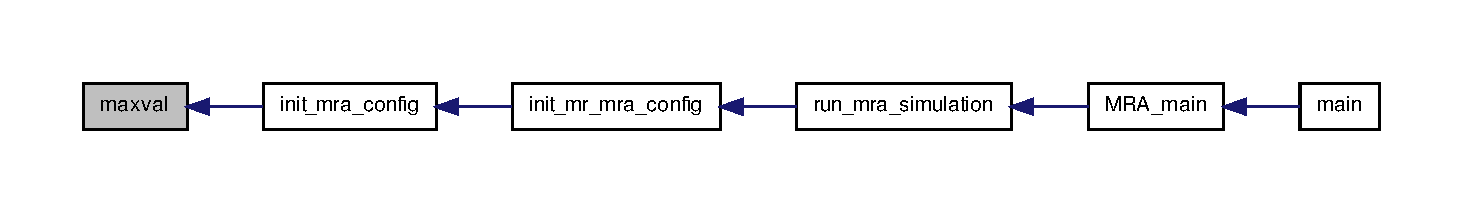
\includegraphics[width=350pt]{common-mra_8h_a411d5133ab6881d40ef4cb44a7a47428_icgraph}
\end{center}
\end{figure}


\hypertarget{common-mra_8h_ad37a02c988c597622a346cb5293243fb}{\index{common-\/mra.\-h@{common-\/mra.\-h}!message\-\_\-is@{message\-\_\-is}}
\index{message\-\_\-is@{message\-\_\-is}!common-mra.h@{common-\/mra.\-h}}
\subsubsection[{message\-\_\-is}]{\setlength{\rightskip}{0pt plus 5cm}int {\bf message\-\_\-is} (
\begin{DoxyParamCaption}
\item[{msg\-\_\-task\-\_\-t}]{msg, }
\item[{const char $\ast$}]{str}
\end{DoxyParamCaption}
)}}\label{common-mra_8h_ad37a02c988c597622a346cb5293243fb}


\-Compare the message from a task with a string. 


\begin{DoxyParams}{\-Parameters}
{\em msg} & \-The message/task. \\
\hline
{\em str} & \-The string to compare with. \\
\hline
\end{DoxyParams}
\begin{DoxyReturn}{\-Returns}
\-A positive value if matches, zero if doesn't. 
\end{DoxyReturn}


\-Here is the caller graph for this function\-:\nopagebreak
\begin{figure}[H]
\begin{center}
\leavevmode
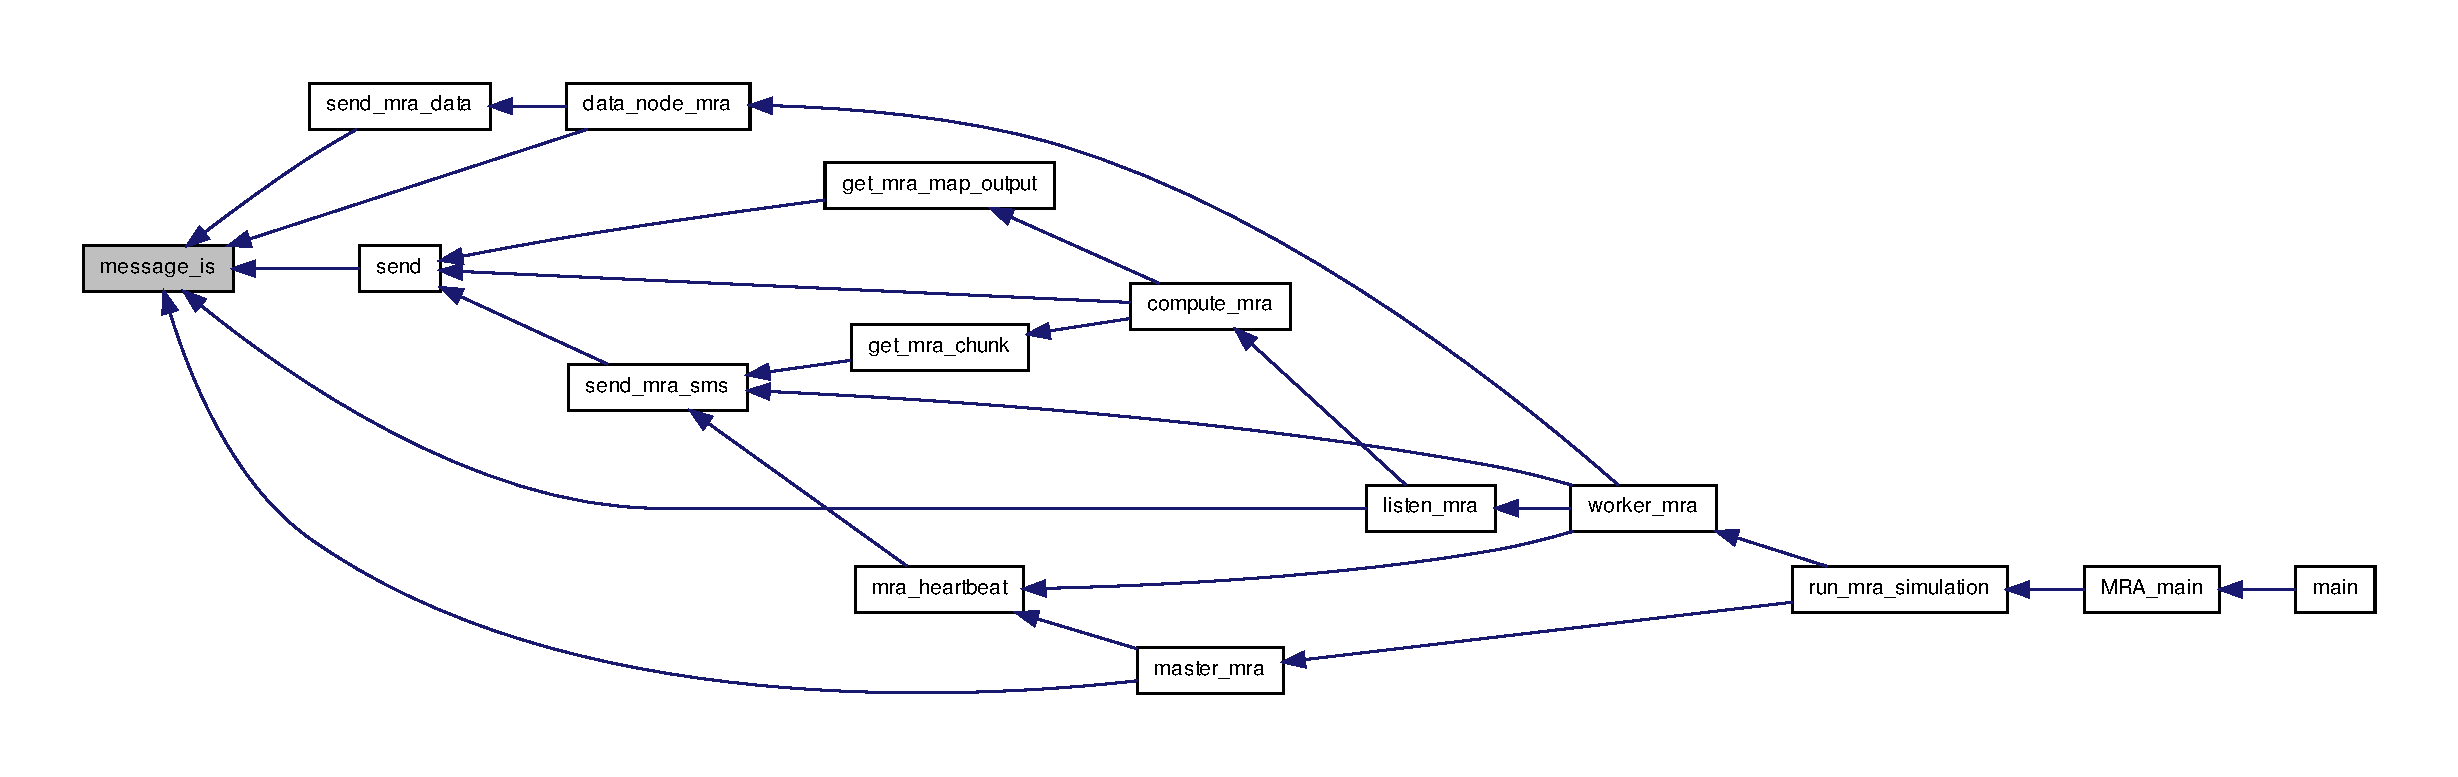
\includegraphics[width=350pt]{common-mra_8h_ad37a02c988c597622a346cb5293243fb_icgraph}
\end{center}
\end{figure}


\hypertarget{common-mra_8h_a6fc60933b9eabe64a880f68eba3131cc}{\index{common-\/mra.\-h@{common-\/mra.\-h}!receive@{receive}}
\index{receive@{receive}!common-mra.h@{common-\/mra.\-h}}
\subsubsection[{receive}]{\setlength{\rightskip}{0pt plus 5cm}msg\-\_\-error\-\_\-t {\bf receive} (
\begin{DoxyParamCaption}
\item[{msg\-\_\-task\-\_\-t $\ast$}]{msg, }
\item[{const char $\ast$}]{mailbox}
\end{DoxyParamCaption}
)}}\label{common-mra_8h_a6fc60933b9eabe64a880f68eba3131cc}


\-Receive a message/task from a mailbox. 


\begin{DoxyParams}{\-Parameters}
{\em msg} & \-Where to store the received message. \\
\hline
{\em mailbox} & \-The mailbox alias. \\
\hline
\end{DoxyParams}
\begin{DoxyReturn}{\-Returns}
\-The status of the transfer. 
\end{DoxyReturn}


\-Here is the caller graph for this function\-:\nopagebreak
\begin{figure}[H]
\begin{center}
\leavevmode
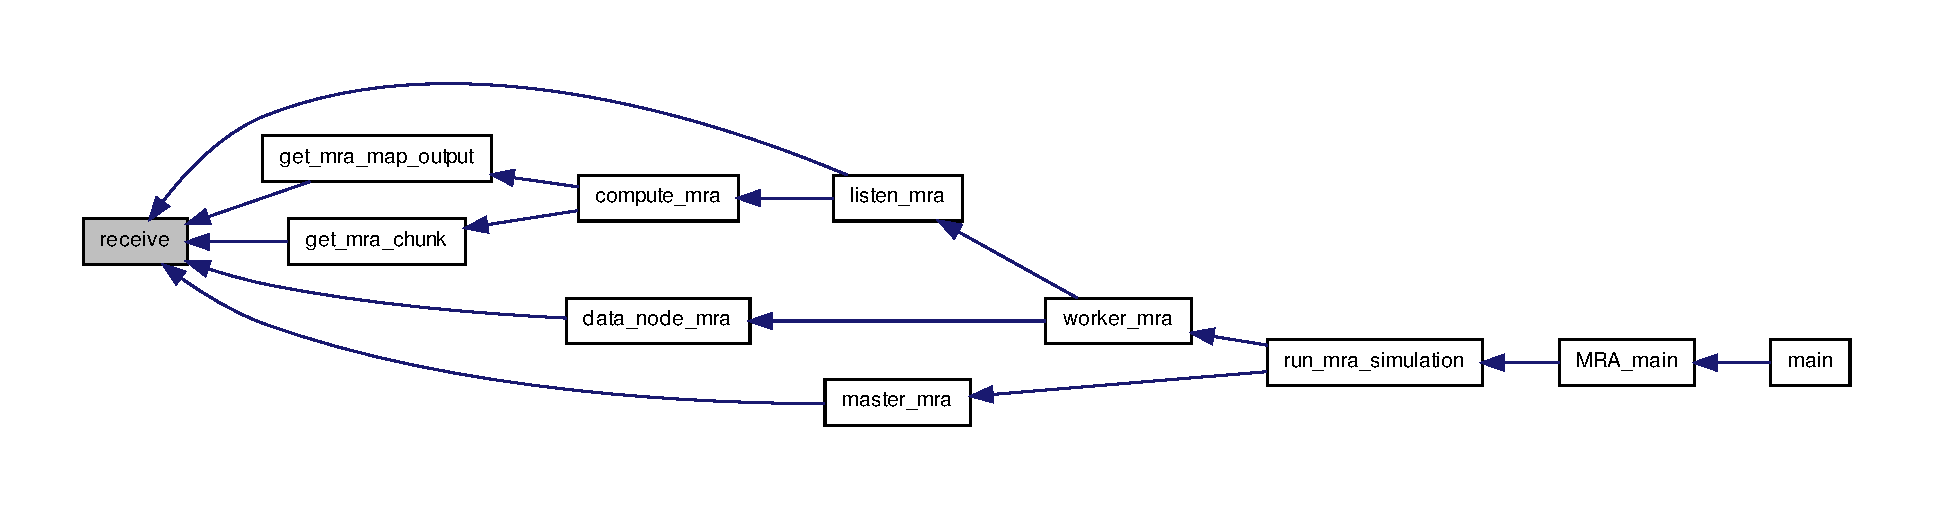
\includegraphics[width=350pt]{common-mra_8h_a6fc60933b9eabe64a880f68eba3131cc_icgraph}
\end{center}
\end{figure}


\hypertarget{common-mra_8h_a8205e98d4874b7e31f138d5016ad1eba}{\index{common-\/mra.\-h@{common-\/mra.\-h}!reduce\-\_\-mra\-\_\-input\-\_\-size@{reduce\-\_\-mra\-\_\-input\-\_\-size}}
\index{reduce\-\_\-mra\-\_\-input\-\_\-size@{reduce\-\_\-mra\-\_\-input\-\_\-size}!common-mra.h@{common-\/mra.\-h}}
\subsubsection[{reduce\-\_\-mra\-\_\-input\-\_\-size}]{\setlength{\rightskip}{0pt plus 5cm}size\-\_\-t {\bf reduce\-\_\-mra\-\_\-input\-\_\-size} (
\begin{DoxyParamCaption}
\item[{size\-\_\-t}]{rid}
\end{DoxyParamCaption}
)}}\label{common-mra_8h_a8205e98d4874b7e31f138d5016ad1eba}


\-Return the input size of a reduce task. 


\begin{DoxyParams}{\-Parameters}
{\em rid} & \-The reduce task \-I\-D. \\
\hline
\end{DoxyParams}
\begin{DoxyReturn}{\-Returns}
\-The task input size in bytes. 
\end{DoxyReturn}


\-Here is the caller graph for this function\-:\nopagebreak
\begin{figure}[H]
\begin{center}
\leavevmode
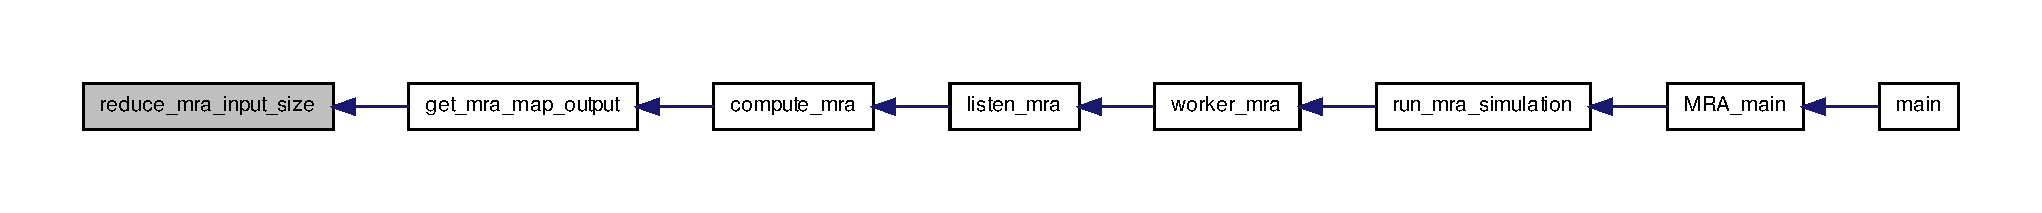
\includegraphics[width=350pt]{common-mra_8h_a8205e98d4874b7e31f138d5016ad1eba_icgraph}
\end{center}
\end{figure}


\hypertarget{common-mra_8h_a385b12669d8faf7b5cdb54c1ae597e1c}{\index{common-\/mra.\-h@{common-\/mra.\-h}!send@{send}}
\index{send@{send}!common-mra.h@{common-\/mra.\-h}}
\subsubsection[{send}]{\setlength{\rightskip}{0pt plus 5cm}msg\-\_\-error\-\_\-t {\bf send} (
\begin{DoxyParamCaption}
\item[{const char $\ast$}]{str, }
\item[{double}]{cpu, }
\item[{double}]{net, }
\item[{void $\ast$}]{data, }
\item[{const char $\ast$}]{mailbox}
\end{DoxyParamCaption}
)}}\label{common-mra_8h_a385b12669d8faf7b5cdb54c1ae597e1c}


\-Send a message/task. 


\begin{DoxyParams}{\-Parameters}
{\em str} & \-The message. \\
\hline
{\em cpu} & \-The amount of cpu required by the task. \\
\hline
{\em net} & \-The message size in bytes. \\
\hline
{\em data} & \-Any data to attatch to the message. \\
\hline
{\em mailbox} & \-The destination mailbox alias. \\
\hline
\end{DoxyParams}
\begin{DoxyReturn}{\-Returns}
\-The \-M\-S\-G status of the operation. 
\end{DoxyReturn}


\-Here is the call graph for this function\-:\nopagebreak
\begin{figure}[H]
\begin{center}
\leavevmode
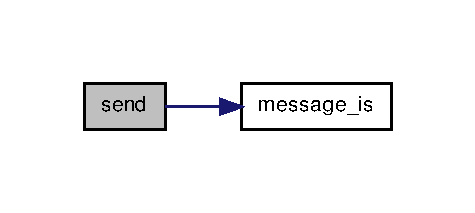
\includegraphics[width=228pt]{common-mra_8h_a385b12669d8faf7b5cdb54c1ae597e1c_cgraph}
\end{center}
\end{figure}




\-Here is the caller graph for this function\-:\nopagebreak
\begin{figure}[H]
\begin{center}
\leavevmode
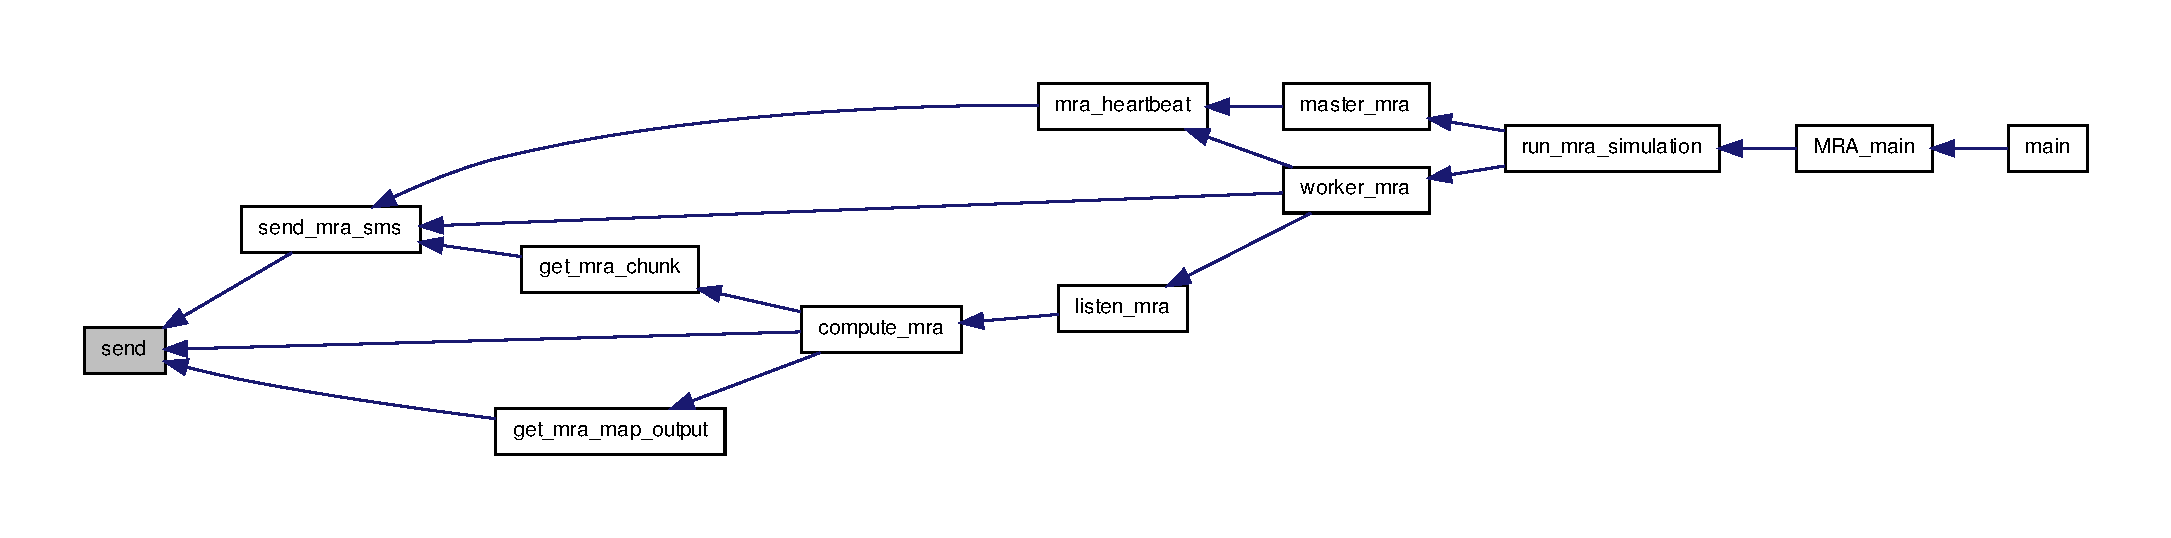
\includegraphics[width=350pt]{common-mra_8h_a385b12669d8faf7b5cdb54c1ae597e1c_icgraph}
\end{center}
\end{figure}


\hypertarget{common-mra_8h_a305ac8e3389f94106990aa3c52c91416}{\index{common-\/mra.\-h@{common-\/mra.\-h}!send\-\_\-mra\-\_\-sms@{send\-\_\-mra\-\_\-sms}}
\index{send\-\_\-mra\-\_\-sms@{send\-\_\-mra\-\_\-sms}!common-mra.h@{common-\/mra.\-h}}
\subsubsection[{send\-\_\-mra\-\_\-sms}]{\setlength{\rightskip}{0pt plus 5cm}msg\-\_\-error\-\_\-t {\bf send\-\_\-mra\-\_\-sms} (
\begin{DoxyParamCaption}
\item[{const char $\ast$}]{str, }
\item[{const char $\ast$}]{mailbox}
\end{DoxyParamCaption}
)}}\label{common-mra_8h_a305ac8e3389f94106990aa3c52c91416}


\-Send a short message, of size zero. 


\begin{DoxyParams}{\-Parameters}
{\em str} & \-The message. \\
\hline
{\em mailbox} & \-The destination mailbox alias. \\
\hline
\end{DoxyParams}
\begin{DoxyReturn}{\-Returns}
\-The \-M\-S\-G status of the operation. 
\end{DoxyReturn}


\-Here is the call graph for this function\-:\nopagebreak
\begin{figure}[H]
\begin{center}
\leavevmode
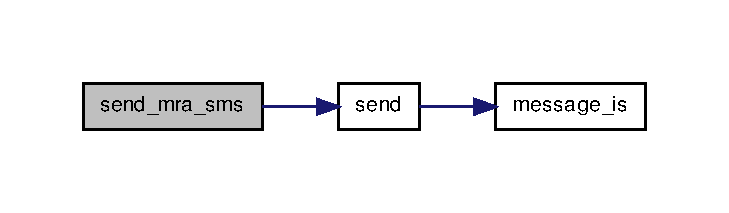
\includegraphics[width=350pt]{common-mra_8h_a305ac8e3389f94106990aa3c52c91416_cgraph}
\end{center}
\end{figure}




\-Here is the caller graph for this function\-:\nopagebreak
\begin{figure}[H]
\begin{center}
\leavevmode
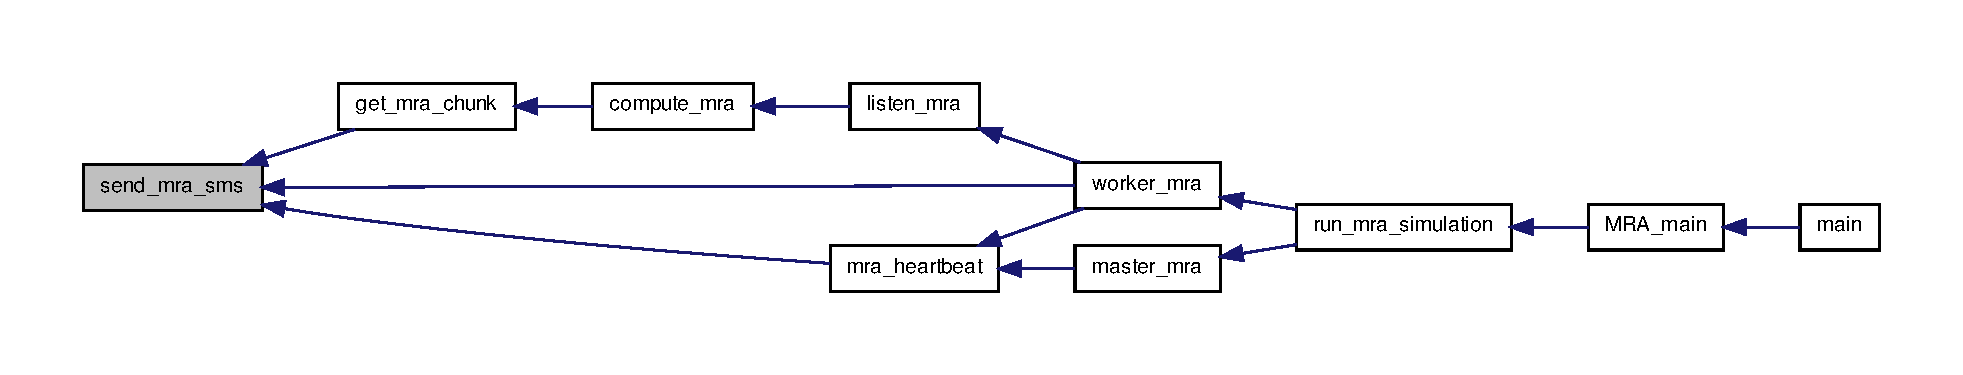
\includegraphics[width=350pt]{common-mra_8h_a305ac8e3389f94106990aa3c52c91416_icgraph}
\end{center}
\end{figure}




\subsection{\-Variable \-Documentation}
\hypertarget{common-mra_8h_afc43959c8dc45a0582a605a20e83aa0d}{\index{common-\/mra.\-h@{common-\/mra.\-h}!avg\-\_\-task\-\_\-exec\-\_\-map@{avg\-\_\-task\-\_\-exec\-\_\-map}}
\index{avg\-\_\-task\-\_\-exec\-\_\-map@{avg\-\_\-task\-\_\-exec\-\_\-map}!common-mra.h@{common-\/mra.\-h}}
\subsubsection[{avg\-\_\-task\-\_\-exec\-\_\-map}]{\setlength{\rightskip}{0pt plus 5cm}double$\ast$ {\bf avg\-\_\-task\-\_\-exec\-\_\-map}}}\label{common-mra_8h_afc43959c8dc45a0582a605a20e83aa0d}
\hypertarget{common-mra_8h_ad5b90869efe31de6176f099e9cf99de5}{\index{common-\/mra.\-h@{common-\/mra.\-h}!avg\-\_\-task\-\_\-exec\-\_\-reduce@{avg\-\_\-task\-\_\-exec\-\_\-reduce}}
\index{avg\-\_\-task\-\_\-exec\-\_\-reduce@{avg\-\_\-task\-\_\-exec\-\_\-reduce}!common-mra.h@{common-\/mra.\-h}}
\subsubsection[{avg\-\_\-task\-\_\-exec\-\_\-reduce}]{\setlength{\rightskip}{0pt plus 5cm}double$\ast$ {\bf avg\-\_\-task\-\_\-exec\-\_\-reduce}}}\label{common-mra_8h_ad5b90869efe31de6176f099e9cf99de5}
\hypertarget{common-mra_8h_a1860c3de3eef8309ccc6b068eb3a08f6}{\index{common-\/mra.\-h@{common-\/mra.\-h}!config\-\_\-mra@{config\-\_\-mra}}
\index{config\-\_\-mra@{config\-\_\-mra}!common-mra.h@{common-\/mra.\-h}}
\subsubsection[{config\-\_\-mra}]{\setlength{\rightskip}{0pt plus 5cm}struct {\bf config\-\_\-s}  {\bf config\-\_\-mra}}}\label{common-mra_8h_a1860c3de3eef8309ccc6b068eb3a08f6}
\hypertarget{common-mra_8h_a25cc609dae2875ebd3e01dec54626409}{\index{common-\/mra.\-h@{common-\/mra.\-h}!dist\-\_\-bruta@{dist\-\_\-bruta}}
\index{dist\-\_\-bruta@{dist\-\_\-bruta}!common-mra.h@{common-\/mra.\-h}}
\subsubsection[{dist\-\_\-bruta}]{\setlength{\rightskip}{0pt plus 5cm}int$\ast$ {\bf dist\-\_\-bruta}}}\label{common-mra_8h_a25cc609dae2875ebd3e01dec54626409}


\-Initialize dist\-\_\-bruta, task\-\_\-exec, avg\-\_\-task\-\_\-exec. 

\hypertarget{common-mra_8h_a40c5dda5ba96917071a5d075c25444b2}{\index{common-\/mra.\-h@{common-\/mra.\-h}!\-Fg@{\-Fg}}
\index{\-Fg@{\-Fg}!common-mra.h@{common-\/mra.\-h}}
\subsubsection[{\-Fg}]{\setlength{\rightskip}{0pt plus 5cm}int {\bf \-Fg}}}\label{common-mra_8h_a40c5dda5ba96917071a5d075c25444b2}
\hypertarget{common-mra_8h_a110d69f20330d00e3fa77e764feb5d54}{\index{common-\/mra.\-h@{common-\/mra.\-h}!job\-\_\-mra@{job\-\_\-mra}}
\index{job\-\_\-mra@{job\-\_\-mra}!common-mra.h@{common-\/mra.\-h}}
\subsubsection[{job\-\_\-mra}]{\setlength{\rightskip}{0pt plus 5cm}struct {\bf job\-\_\-s}  {\bf job\-\_\-mra}}}\label{common-mra_8h_a110d69f20330d00e3fa77e764feb5d54}
\hypertarget{common-mra_8h_aaa0bc264a86ff2516e39fdba05b72b66}{\index{common-\/mra.\-h@{common-\/mra.\-h}!mra\-\_\-perc@{mra\-\_\-perc}}
\index{mra\-\_\-perc@{mra\-\_\-perc}!common-mra.h@{common-\/mra.\-h}}
\subsubsection[{mra\-\_\-perc}]{\setlength{\rightskip}{0pt plus 5cm}int {\bf mra\-\_\-perc}}}\label{common-mra_8h_aaa0bc264a86ff2516e39fdba05b72b66}
\hypertarget{common-mra_8h_aa526e398bda7952ec6bcc5c33d39abac}{\index{common-\/mra.\-h@{common-\/mra.\-h}!stats\-\_\-mra@{stats\-\_\-mra}}
\index{stats\-\_\-mra@{stats\-\_\-mra}!common-mra.h@{common-\/mra.\-h}}
\subsubsection[{stats\-\_\-mra}]{\setlength{\rightskip}{0pt plus 5cm}struct {\bf stats\-\_\-s}  {\bf stats\-\_\-mra}}}\label{common-mra_8h_aa526e398bda7952ec6bcc5c33d39abac}
\hypertarget{common-mra_8h_a3643aab6c35479d8e7c2f7e46bdb04b8}{\index{common-\/mra.\-h@{common-\/mra.\-h}!task\-\_\-exec@{task\-\_\-exec}}
\index{task\-\_\-exec@{task\-\_\-exec}!common-mra.h@{common-\/mra.\-h}}
\subsubsection[{task\-\_\-exec}]{\setlength{\rightskip}{0pt plus 5cm}double$\ast$ {\bf task\-\_\-exec}}}\label{common-mra_8h_a3643aab6c35479d8e7c2f7e46bdb04b8}
\hypertarget{common-mra_8h_ad7eb2fd97a2f868b28c25405de9a4e72}{\index{common-\/mra.\-h@{common-\/mra.\-h}!user\-\_\-mra@{user\-\_\-mra}}
\index{user\-\_\-mra@{user\-\_\-mra}!common-mra.h@{common-\/mra.\-h}}
\subsubsection[{user\-\_\-mra}]{\setlength{\rightskip}{0pt plus 5cm}struct {\bf user\-\_\-s}  {\bf user\-\_\-mra}}}\label{common-mra_8h_ad7eb2fd97a2f868b28c25405de9a4e72}

\hypertarget{dfs-mra_8h}{\section{include/dfs-\/mra.h \-File \-Reference}
\label{dfs-mra_8h}\index{include/dfs-\/mra.\-h@{include/dfs-\/mra.\-h}}
}
\-This graph shows which files directly or indirectly include this file\-:\nopagebreak
\begin{figure}[H]
\begin{center}
\leavevmode
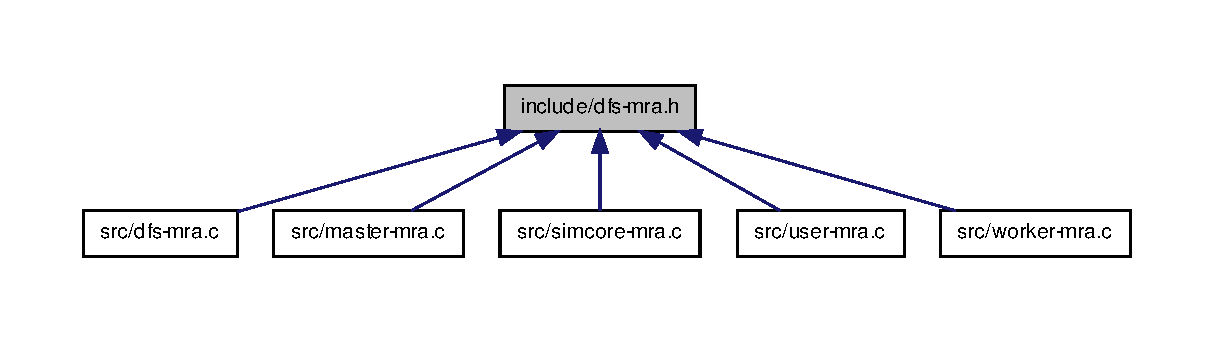
\includegraphics[width=350pt]{dfs-mra_8h__dep__incl}
\end{center}
\end{figure}
\subsection*{\-Functions}
\begin{DoxyCompactItemize}
\item 
void \hyperlink{dfs-mra_8h_a23d972ed8df40ef6ff709f57e3944042}{distribute\-\_\-data\-\_\-mra} (void)
\begin{DoxyCompactList}\small\item\em \-Distribute chunks (and replicas) to \-Data\-Nodes. \end{DoxyCompactList}\item 
void \hyperlink{dfs-mra_8h_ac144b7da2b0cb2e76cf7226740c54dc1}{default\-\_\-mra\-\_\-dfs\-\_\-f} (char $\ast$$\ast$mra\-\_\-dfs\-\_\-matrix, size\-\_\-t chunks, size\-\_\-t workers\-\_\-mra, int replicas)
\begin{DoxyCompactList}\small\item\em \-Default data distribution algorithm. \end{DoxyCompactList}\item 
size\-\_\-t \hyperlink{dfs-mra_8h_a3f8eddb9dd6200115f7d88325537035e}{find\-\_\-random\-\_\-mra\-\_\-chunk\-\_\-owner} (int cid)
\begin{DoxyCompactList}\small\item\em \-Choose a random \-Data\-Node that owns a specific chunk. \end{DoxyCompactList}\item 
int \hyperlink{dfs-mra_8h_a86d9bef64a7e145c3e00de4e74e8d1c6}{data\-\_\-node\-\_\-mra} (int argc, char $\ast$argv\mbox{[}$\,$\mbox{]})
\begin{DoxyCompactList}\small\item\em \-Data\-Node main function. \end{DoxyCompactList}\end{DoxyCompactItemize}
\subsection*{\-Variables}
\begin{DoxyCompactItemize}
\item 
char $\ast$$\ast$ \hyperlink{dfs-mra_8h_a03bfd03cf290b4a74e89090bde97bd2f}{chunk\-\_\-owner\-\_\-mra}
\begin{DoxyCompactList}\small\item\em \-Matrix that maps chunks to workers. \end{DoxyCompactList}\end{DoxyCompactItemize}


\subsection{\-Function \-Documentation}
\hypertarget{dfs-mra_8h_a86d9bef64a7e145c3e00de4e74e8d1c6}{\index{dfs-\/mra.\-h@{dfs-\/mra.\-h}!data\-\_\-node\-\_\-mra@{data\-\_\-node\-\_\-mra}}
\index{data\-\_\-node\-\_\-mra@{data\-\_\-node\-\_\-mra}!dfs-mra.h@{dfs-\/mra.\-h}}
\subsubsection[{data\-\_\-node\-\_\-mra}]{\setlength{\rightskip}{0pt plus 5cm}int {\bf data\-\_\-node\-\_\-mra} (
\begin{DoxyParamCaption}
\item[{int}]{argc, }
\item[{char $\ast$}]{argv\mbox{[}$\,$\mbox{]}}
\end{DoxyParamCaption}
)}}\label{dfs-mra_8h_a86d9bef64a7e145c3e00de4e74e8d1c6}


\-Data\-Node main function. 

\-Process that listens for data requests. 

\-Here is the call graph for this function\-:\nopagebreak
\begin{figure}[H]
\begin{center}
\leavevmode
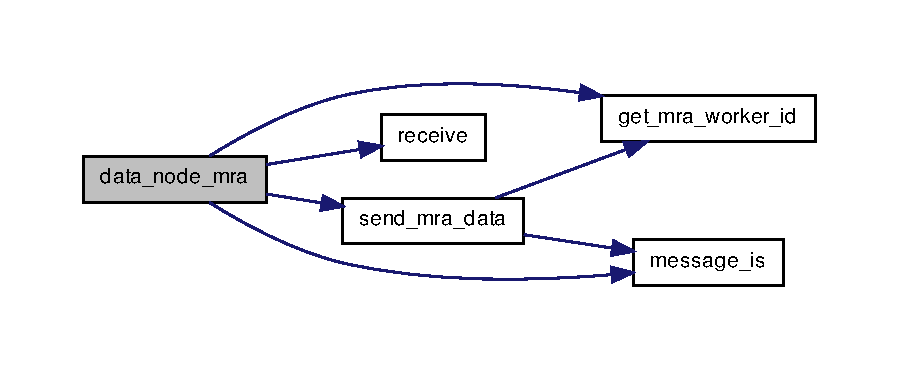
\includegraphics[width=350pt]{dfs-mra_8h_a86d9bef64a7e145c3e00de4e74e8d1c6_cgraph}
\end{center}
\end{figure}




\-Here is the caller graph for this function\-:\nopagebreak
\begin{figure}[H]
\begin{center}
\leavevmode
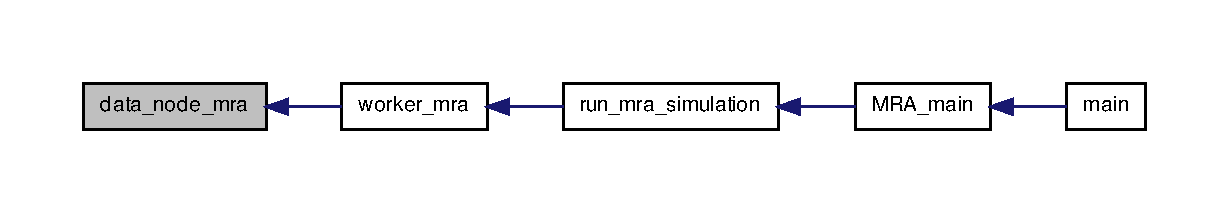
\includegraphics[width=350pt]{dfs-mra_8h_a86d9bef64a7e145c3e00de4e74e8d1c6_icgraph}
\end{center}
\end{figure}


\hypertarget{dfs-mra_8h_ac144b7da2b0cb2e76cf7226740c54dc1}{\index{dfs-\/mra.\-h@{dfs-\/mra.\-h}!default\-\_\-mra\-\_\-dfs\-\_\-f@{default\-\_\-mra\-\_\-dfs\-\_\-f}}
\index{default\-\_\-mra\-\_\-dfs\-\_\-f@{default\-\_\-mra\-\_\-dfs\-\_\-f}!dfs-mra.h@{dfs-\/mra.\-h}}
\subsubsection[{default\-\_\-mra\-\_\-dfs\-\_\-f}]{\setlength{\rightskip}{0pt plus 5cm}void {\bf default\-\_\-mra\-\_\-dfs\-\_\-f} (
\begin{DoxyParamCaption}
\item[{char $\ast$$\ast$}]{mra\-\_\-dfs\-\_\-matrix, }
\item[{size\-\_\-t}]{chunks, }
\item[{size\-\_\-t}]{workers\-\_\-mra, }
\item[{int}]{replicas}
\end{DoxyParamCaption}
)}}\label{dfs-mra_8h_ac144b7da2b0cb2e76cf7226740c54dc1}


\-Default data distribution algorithm. 

de workers -\/-\/$>$ workers\-\_\-hosts\mbox{[}id\mbox{]} (array)  capacidade -\/-\/$>$ \-M\-S\-G\-\_\-get\-\_\-host\-\_\-speed (config\-\_\-mra.\-workers\mbox{[}owner\mbox{]})  -\/-\/$>$ \-Calcula a capacidade computacional relativa de cada worker baseado na capacidade total da grid.  -\/-\/$>$ É o array com as tribuições brutas, antes do ajuste de menor te\-\_\-exec  -\/-\/$>$ É o array com o valor de previsão de término de todas as tarefas distribuídas ao worker;  -\/-\/$>$ É o array com o tempo que será utilizado para encontar a melhor distribuição  -\/-\/$>$ É o array que contém o tempo de cada worker para executar uma tarefa computacional padrão

config\-\_\-mra.\-slots\-\_\-mra\mbox{[}\-M\-R\-A\-\_\-\-M\-A\-P\mbox{]};

-\/-\/$>$ verifica qual é o maior tempo de execução previsto

\-Ajuste de \-Força \-Bruta com uma \-Otimização \-Combinatória para obter uma distribuição de chunks com o menor tempo de execução possível

\-Here is the caller graph for this function\-:\nopagebreak
\begin{figure}[H]
\begin{center}
\leavevmode
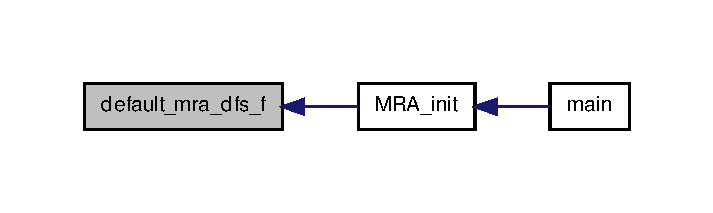
\includegraphics[width=342pt]{dfs-mra_8h_ac144b7da2b0cb2e76cf7226740c54dc1_icgraph}
\end{center}
\end{figure}


\hypertarget{dfs-mra_8h_a23d972ed8df40ef6ff709f57e3944042}{\index{dfs-\/mra.\-h@{dfs-\/mra.\-h}!distribute\-\_\-data\-\_\-mra@{distribute\-\_\-data\-\_\-mra}}
\index{distribute\-\_\-data\-\_\-mra@{distribute\-\_\-data\-\_\-mra}!dfs-mra.h@{dfs-\/mra.\-h}}
\subsubsection[{distribute\-\_\-data\-\_\-mra}]{\setlength{\rightskip}{0pt plus 5cm}void {\bf distribute\-\_\-data\-\_\-mra} (
\begin{DoxyParamCaption}
\item[{void}]{}
\end{DoxyParamCaption}
)}}\label{dfs-mra_8h_a23d972ed8df40ef6ff709f57e3944042}


\-Distribute chunks (and replicas) to \-Data\-Nodes. 



\-Here is the caller graph for this function\-:\nopagebreak
\begin{figure}[H]
\begin{center}
\leavevmode
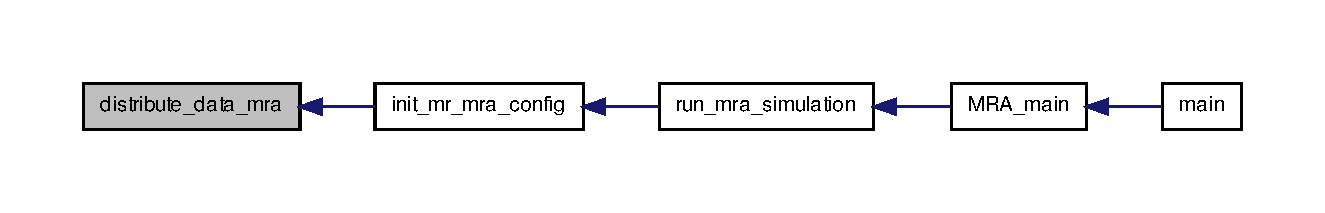
\includegraphics[width=350pt]{dfs-mra_8h_a23d972ed8df40ef6ff709f57e3944042_icgraph}
\end{center}
\end{figure}


\hypertarget{dfs-mra_8h_a3f8eddb9dd6200115f7d88325537035e}{\index{dfs-\/mra.\-h@{dfs-\/mra.\-h}!find\-\_\-random\-\_\-mra\-\_\-chunk\-\_\-owner@{find\-\_\-random\-\_\-mra\-\_\-chunk\-\_\-owner}}
\index{find\-\_\-random\-\_\-mra\-\_\-chunk\-\_\-owner@{find\-\_\-random\-\_\-mra\-\_\-chunk\-\_\-owner}!dfs-mra.h@{dfs-\/mra.\-h}}
\subsubsection[{find\-\_\-random\-\_\-mra\-\_\-chunk\-\_\-owner}]{\setlength{\rightskip}{0pt plus 5cm}size\-\_\-t {\bf find\-\_\-random\-\_\-mra\-\_\-chunk\-\_\-owner} (
\begin{DoxyParamCaption}
\item[{int}]{cid}
\end{DoxyParamCaption}
)}}\label{dfs-mra_8h_a3f8eddb9dd6200115f7d88325537035e}


\-Choose a random \-Data\-Node that owns a specific chunk. 


\begin{DoxyParams}{\-Parameters}
{\em cid} & \-The chunk \-I\-D. \\
\hline
\end{DoxyParams}
\begin{DoxyReturn}{\-Returns}
\-The \-I\-D of the \-Data\-Node.
\end{DoxyReturn}
\-Distribution of \-Data \-Replication 
\begin{DoxyParams}{\-Parameters}
{\em cid} & \-The chunk \-I\-D. \\
\hline
\end{DoxyParams}
\begin{DoxyReturn}{\-Returns}
\-The \-I\-D of the \-Data\-Node. 
\end{DoxyReturn}


\-Here is the caller graph for this function\-:\nopagebreak
\begin{figure}[H]
\begin{center}
\leavevmode
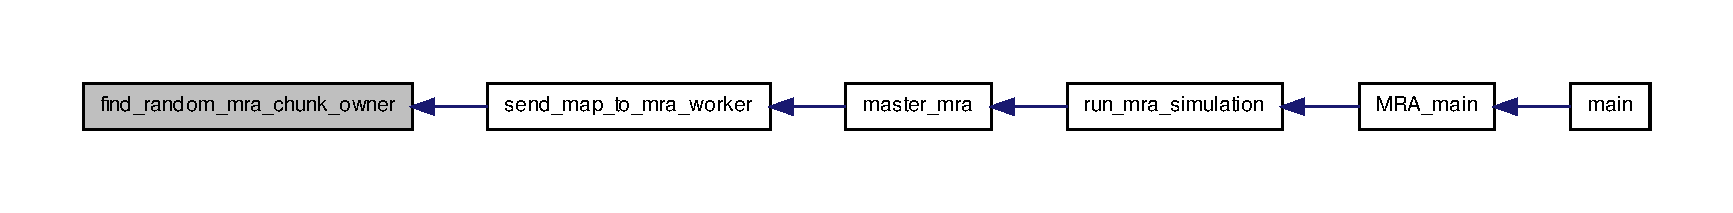
\includegraphics[width=350pt]{dfs-mra_8h_a3f8eddb9dd6200115f7d88325537035e_icgraph}
\end{center}
\end{figure}




\subsection{\-Variable \-Documentation}
\hypertarget{dfs-mra_8h_a03bfd03cf290b4a74e89090bde97bd2f}{\index{dfs-\/mra.\-h@{dfs-\/mra.\-h}!chunk\-\_\-owner\-\_\-mra@{chunk\-\_\-owner\-\_\-mra}}
\index{chunk\-\_\-owner\-\_\-mra@{chunk\-\_\-owner\-\_\-mra}!dfs-mra.h@{dfs-\/mra.\-h}}
\subsubsection[{chunk\-\_\-owner\-\_\-mra}]{\setlength{\rightskip}{0pt plus 5cm}char$\ast$$\ast$ {\bf chunk\-\_\-owner\-\_\-mra}}}\label{dfs-mra_8h_a03bfd03cf290b4a74e89090bde97bd2f}


\-Matrix that maps chunks to workers. 


\hypertarget{mra_8h}{\section{include/mra.h \-File \-Reference}
\label{mra_8h}\index{include/mra.\-h@{include/mra.\-h}}
}
{\ttfamily \#include $<$stdlib.\-h$>$}\*
\-Include dependency graph for mra.\-h\-:
\nopagebreak
\begin{figure}[H]
\begin{center}
\leavevmode
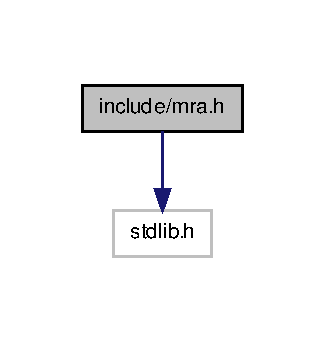
\includegraphics[width=156pt]{mra_8h__incl}
\end{center}
\end{figure}
\-This graph shows which files directly or indirectly include this file\-:
\nopagebreak
\begin{figure}[H]
\begin{center}
\leavevmode
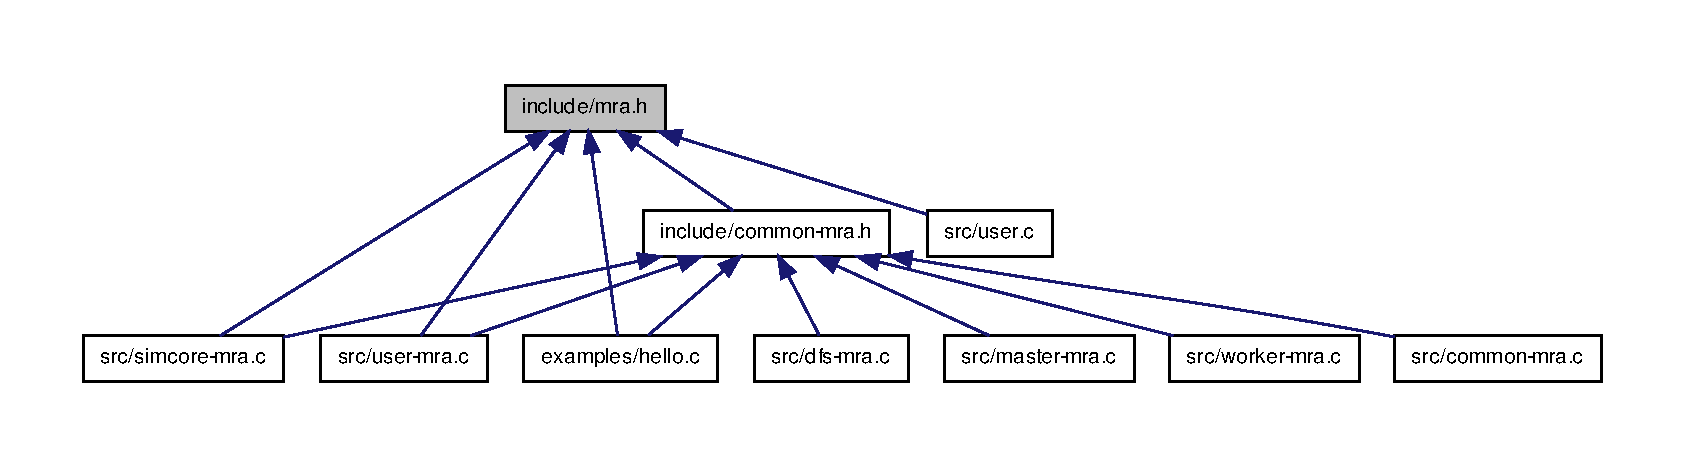
\includegraphics[width=350pt]{mra_8h__dep__incl}
\end{center}
\end{figure}
\subsection*{\-Enumerations}
\begin{DoxyCompactItemize}
\item 
enum \hyperlink{mra_8h_afa14b6e068c0e0b8557777e16f2582f2}{phase\-\_\-e} \{ \hyperlink{mra_8h_afa14b6e068c0e0b8557777e16f2582f2a482af38fffb9ce534a152eb5c2271220}{\-M\-R\-A\-\_\-\-M\-A\-P}, 
\hyperlink{mra_8h_afa14b6e068c0e0b8557777e16f2582f2abdd2882d14d1c93e6e2532ba2f0f4f7b}{\-M\-R\-A\-\_\-\-R\-E\-D\-U\-C\-E}
 \}
\begin{DoxyCompactList}\small\item\em \-Possible execution phases. \end{DoxyCompactList}\end{DoxyCompactItemize}
\subsection*{\-Functions}
\begin{DoxyCompactItemize}
\item 
void \hyperlink{mra_8h_ad32b287f1aaa8708a946e2909023bd66}{\-M\-R\-A\-\_\-init} (void)
\item 
int \hyperlink{mra_8h_a002d713ab68756c7102fdf5d914a30da}{\-M\-R\-A\-\_\-main} (const char $\ast$plat, const char $\ast$depl, const char $\ast$conf)
\item 
void \hyperlink{mra_8h_acffcb0453d48f70652984d90ee689172}{\-M\-R\-A\-\_\-set\-\_\-task\-\_\-mra\-\_\-cost\-\_\-f} (double($\ast$f)(enum \hyperlink{mra_8h_afa14b6e068c0e0b8557777e16f2582f2}{phase\-\_\-e} phase, size\-\_\-t tid, size\-\_\-t wid))
\item 
void \hyperlink{mra_8h_abbd980571ade6f7620d2807e9e05ef8f}{\-M\-R\-A\-\_\-set\-\_\-dfs\-\_\-f} (void($\ast$f)(char $\ast$$\ast$mra\-\_\-dfs\-\_\-matrix, size\-\_\-t chunks, size\-\_\-t workers\-\_\-mra, int replicas))
\item 
void \hyperlink{mra_8h_ac642a851bf0b0df3254a086e12d93ab3}{\-M\-R\-A\-\_\-set\-\_\-map\-\_\-mra\-\_\-output\-\_\-f} (int($\ast$f)(size\-\_\-t mid, size\-\_\-t rid))
\end{DoxyCompactItemize}


\subsection{\-Enumeration \-Type \-Documentation}
\hypertarget{mra_8h_afa14b6e068c0e0b8557777e16f2582f2}{\index{mra.\-h@{mra.\-h}!phase\-\_\-e@{phase\-\_\-e}}
\index{phase\-\_\-e@{phase\-\_\-e}!mra.h@{mra.\-h}}
\subsubsection[{phase\-\_\-e}]{\setlength{\rightskip}{0pt plus 5cm}enum {\bf phase\-\_\-e}}}\label{mra_8h_afa14b6e068c0e0b8557777e16f2582f2}


\-Possible execution phases. 

\begin{Desc}
\item[\-Enumerator\-: ]\par
\begin{description}
\index{\-M\-R\-A\-\_\-\-M\-A\-P@{\-M\-R\-A\-\_\-\-M\-A\-P}!mra.\-h@{mra.\-h}}\index{mra.\-h@{mra.\-h}!\-M\-R\-A\-\_\-\-M\-A\-P@{\-M\-R\-A\-\_\-\-M\-A\-P}}\item[{\em 
\hypertarget{mra_8h_afa14b6e068c0e0b8557777e16f2582f2a482af38fffb9ce534a152eb5c2271220}{\-M\-R\-A\-\_\-\-M\-A\-P}\label{mra_8h_afa14b6e068c0e0b8557777e16f2582f2a482af38fffb9ce534a152eb5c2271220}
}]\index{\-M\-R\-A\-\_\-\-R\-E\-D\-U\-C\-E@{\-M\-R\-A\-\_\-\-R\-E\-D\-U\-C\-E}!mra.\-h@{mra.\-h}}\index{mra.\-h@{mra.\-h}!\-M\-R\-A\-\_\-\-R\-E\-D\-U\-C\-E@{\-M\-R\-A\-\_\-\-R\-E\-D\-U\-C\-E}}\item[{\em 
\hypertarget{mra_8h_afa14b6e068c0e0b8557777e16f2582f2abdd2882d14d1c93e6e2532ba2f0f4f7b}{\-M\-R\-A\-\_\-\-R\-E\-D\-U\-C\-E}\label{mra_8h_afa14b6e068c0e0b8557777e16f2582f2abdd2882d14d1c93e6e2532ba2f0f4f7b}
}]\end{description}
\end{Desc}



\subsection{\-Function \-Documentation}
\hypertarget{mra_8h_ad32b287f1aaa8708a946e2909023bd66}{\index{mra.\-h@{mra.\-h}!\-M\-R\-A\-\_\-init@{\-M\-R\-A\-\_\-init}}
\index{\-M\-R\-A\-\_\-init@{\-M\-R\-A\-\_\-init}!mra.h@{mra.\-h}}
\subsubsection[{\-M\-R\-A\-\_\-init}]{\setlength{\rightskip}{0pt plus 5cm}void {\bf \-M\-R\-A\-\_\-init} (
\begin{DoxyParamCaption}
\item[{void}]{}
\end{DoxyParamCaption}
)}}\label{mra_8h_ad32b287f1aaa8708a946e2909023bd66}


\-Here is the call graph for this function\-:
\nopagebreak
\begin{figure}[H]
\begin{center}
\leavevmode
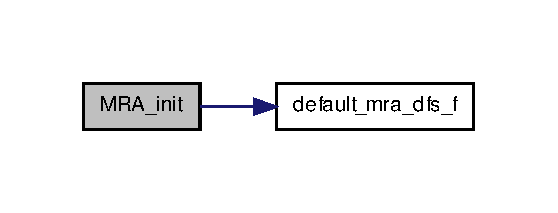
\includegraphics[width=268pt]{mra_8h_ad32b287f1aaa8708a946e2909023bd66_cgraph}
\end{center}
\end{figure}




\-Here is the caller graph for this function\-:
\nopagebreak
\begin{figure}[H]
\begin{center}
\leavevmode
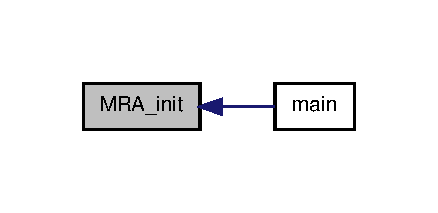
\includegraphics[width=210pt]{mra_8h_ad32b287f1aaa8708a946e2909023bd66_icgraph}
\end{center}
\end{figure}


\hypertarget{mra_8h_a002d713ab68756c7102fdf5d914a30da}{\index{mra.\-h@{mra.\-h}!\-M\-R\-A\-\_\-main@{\-M\-R\-A\-\_\-main}}
\index{\-M\-R\-A\-\_\-main@{\-M\-R\-A\-\_\-main}!mra.h@{mra.\-h}}
\subsubsection[{\-M\-R\-A\-\_\-main}]{\setlength{\rightskip}{0pt plus 5cm}int {\bf \-M\-R\-A\-\_\-main} (
\begin{DoxyParamCaption}
\item[{const char $\ast$}]{plat, }
\item[{const char $\ast$}]{depl, }
\item[{const char $\ast$}]{conf}
\end{DoxyParamCaption}
)}}\label{mra_8h_a002d713ab68756c7102fdf5d914a30da}


\-Here is the call graph for this function\-:
\nopagebreak
\begin{figure}[H]
\begin{center}
\leavevmode
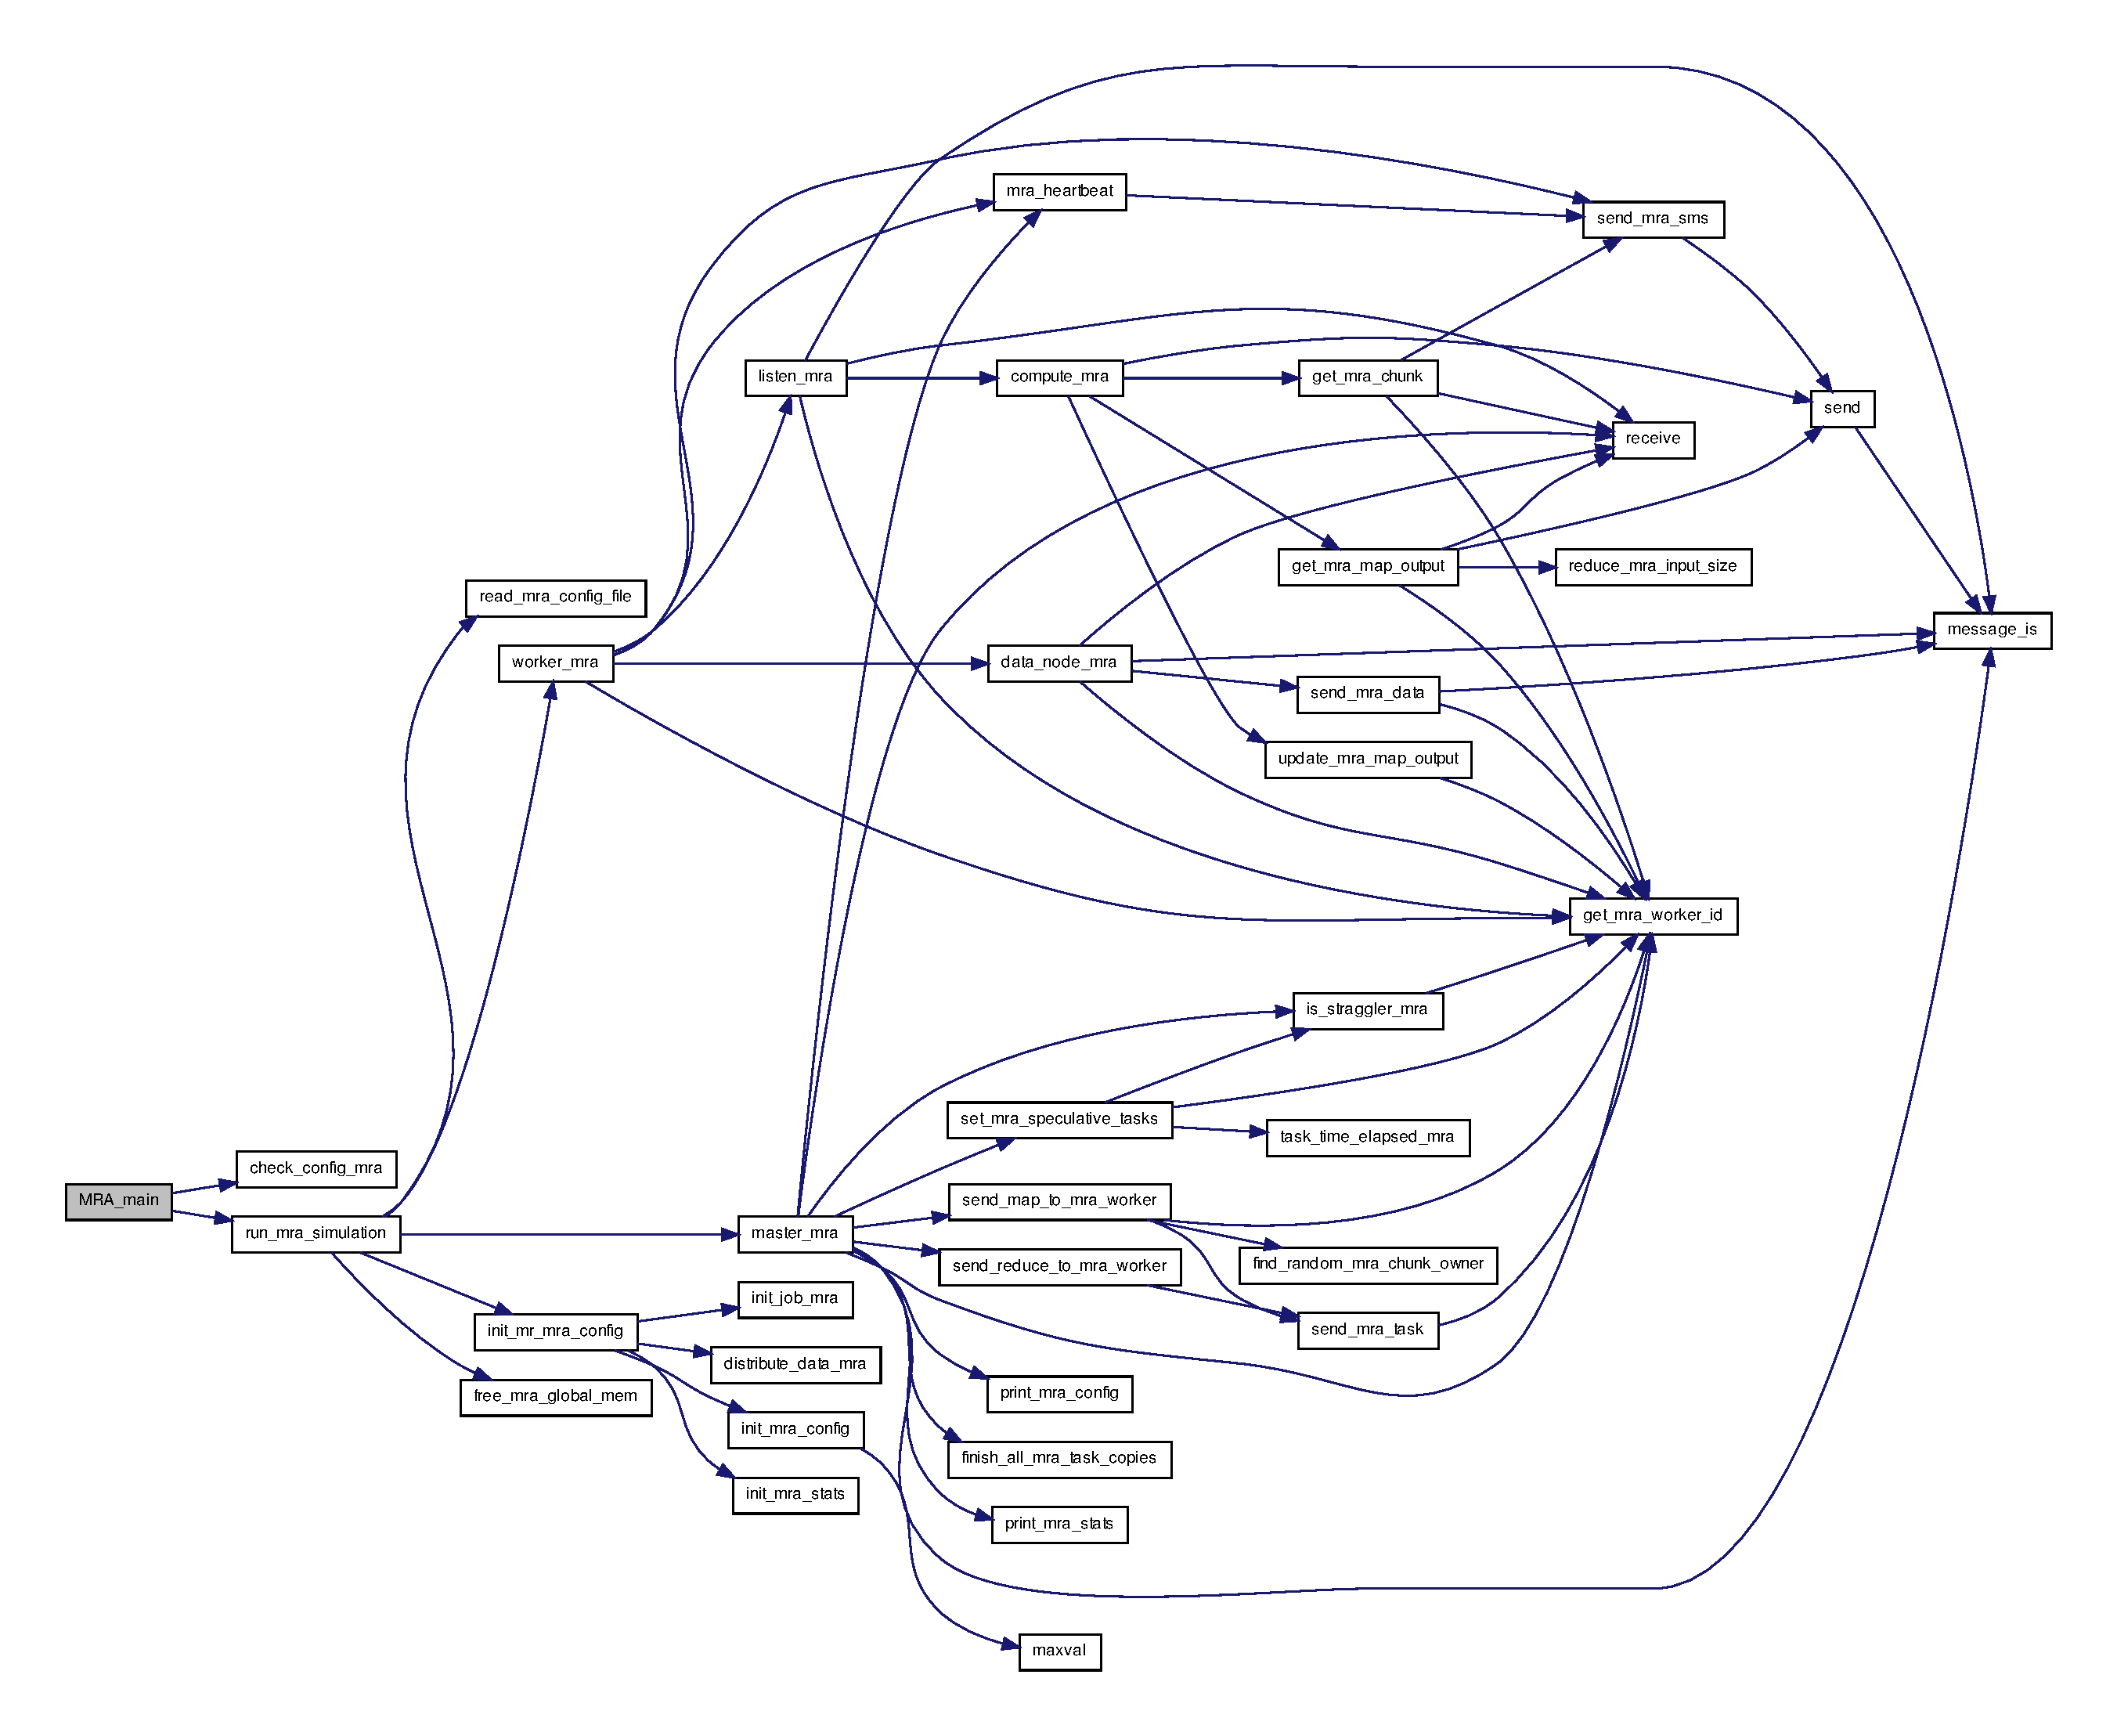
\includegraphics[width=350pt]{mra_8h_a002d713ab68756c7102fdf5d914a30da_cgraph}
\end{center}
\end{figure}




\-Here is the caller graph for this function\-:
\nopagebreak
\begin{figure}[H]
\begin{center}
\leavevmode
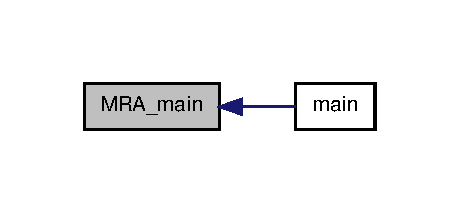
\includegraphics[width=220pt]{mra_8h_a002d713ab68756c7102fdf5d914a30da_icgraph}
\end{center}
\end{figure}


\hypertarget{mra_8h_abbd980571ade6f7620d2807e9e05ef8f}{\index{mra.\-h@{mra.\-h}!\-M\-R\-A\-\_\-set\-\_\-dfs\-\_\-f@{\-M\-R\-A\-\_\-set\-\_\-dfs\-\_\-f}}
\index{\-M\-R\-A\-\_\-set\-\_\-dfs\-\_\-f@{\-M\-R\-A\-\_\-set\-\_\-dfs\-\_\-f}!mra.h@{mra.\-h}}
\subsubsection[{\-M\-R\-A\-\_\-set\-\_\-dfs\-\_\-f}]{\setlength{\rightskip}{0pt plus 5cm}void {\bf \-M\-R\-A\-\_\-set\-\_\-dfs\-\_\-f} (
\begin{DoxyParamCaption}
\item[{void($\ast$)(char $\ast$$\ast$mra\-\_\-dfs\-\_\-matrix, size\-\_\-t chunks, size\-\_\-t workers\-\_\-mra, int replicas)}]{f}
\end{DoxyParamCaption}
)}}\label{mra_8h_abbd980571ade6f7620d2807e9e05ef8f}
\hypertarget{mra_8h_ac642a851bf0b0df3254a086e12d93ab3}{\index{mra.\-h@{mra.\-h}!\-M\-R\-A\-\_\-set\-\_\-map\-\_\-mra\-\_\-output\-\_\-f@{\-M\-R\-A\-\_\-set\-\_\-map\-\_\-mra\-\_\-output\-\_\-f}}
\index{\-M\-R\-A\-\_\-set\-\_\-map\-\_\-mra\-\_\-output\-\_\-f@{\-M\-R\-A\-\_\-set\-\_\-map\-\_\-mra\-\_\-output\-\_\-f}!mra.h@{mra.\-h}}
\subsubsection[{\-M\-R\-A\-\_\-set\-\_\-map\-\_\-mra\-\_\-output\-\_\-f}]{\setlength{\rightskip}{0pt plus 5cm}void {\bf \-M\-R\-A\-\_\-set\-\_\-map\-\_\-mra\-\_\-output\-\_\-f} (
\begin{DoxyParamCaption}
\item[{int($\ast$)(size\-\_\-t mid, size\-\_\-t rid)}]{f}
\end{DoxyParamCaption}
)}}\label{mra_8h_ac642a851bf0b0df3254a086e12d93ab3}


\-Here is the caller graph for this function\-:
\nopagebreak
\begin{figure}[H]
\begin{center}
\leavevmode
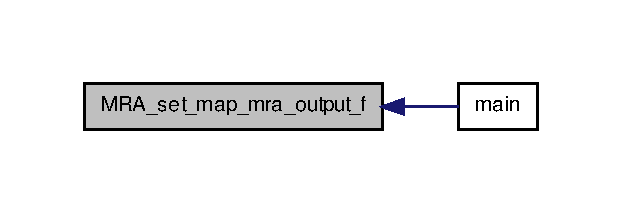
\includegraphics[width=298pt]{mra_8h_ac642a851bf0b0df3254a086e12d93ab3_icgraph}
\end{center}
\end{figure}


\hypertarget{mra_8h_acffcb0453d48f70652984d90ee689172}{\index{mra.\-h@{mra.\-h}!\-M\-R\-A\-\_\-set\-\_\-task\-\_\-mra\-\_\-cost\-\_\-f@{\-M\-R\-A\-\_\-set\-\_\-task\-\_\-mra\-\_\-cost\-\_\-f}}
\index{\-M\-R\-A\-\_\-set\-\_\-task\-\_\-mra\-\_\-cost\-\_\-f@{\-M\-R\-A\-\_\-set\-\_\-task\-\_\-mra\-\_\-cost\-\_\-f}!mra.h@{mra.\-h}}
\subsubsection[{\-M\-R\-A\-\_\-set\-\_\-task\-\_\-mra\-\_\-cost\-\_\-f}]{\setlength{\rightskip}{0pt plus 5cm}void {\bf \-M\-R\-A\-\_\-set\-\_\-task\-\_\-mra\-\_\-cost\-\_\-f} (
\begin{DoxyParamCaption}
\item[{double($\ast$)(enum {\bf phase\-\_\-e} phase, size\-\_\-t tid, size\-\_\-t wid)}]{f}
\end{DoxyParamCaption}
)}}\label{mra_8h_acffcb0453d48f70652984d90ee689172}


\-Here is the caller graph for this function\-:
\nopagebreak
\begin{figure}[H]
\begin{center}
\leavevmode
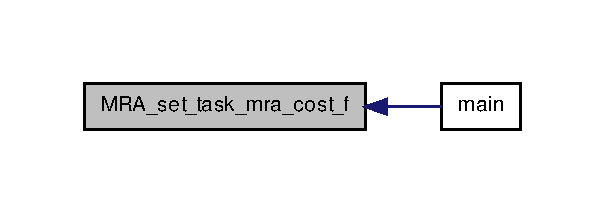
\includegraphics[width=290pt]{mra_8h_acffcb0453d48f70652984d90ee689172_icgraph}
\end{center}
\end{figure}



\hypertarget{worker-mra_8h}{\section{include/worker-\/mra.h \-File \-Reference}
\label{worker-mra_8h}\index{include/worker-\/mra.\-h@{include/worker-\/mra.\-h}}
}
\-This graph shows which files directly or indirectly include this file\-:\nopagebreak
\begin{figure}[H]
\begin{center}
\leavevmode
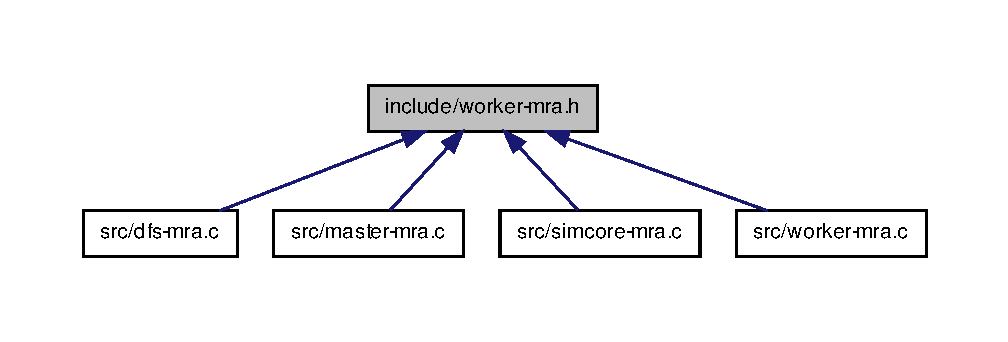
\includegraphics[width=350pt]{worker-mra_8h__dep__incl}
\end{center}
\end{figure}
\subsection*{\-Data \-Structures}
\begin{DoxyCompactItemize}
\item 
struct \hyperlink{structw__info__s}{w\-\_\-info\-\_\-s}
\end{DoxyCompactItemize}
\subsection*{\-Defines}
\begin{DoxyCompactItemize}
\item 
\#define \hyperlink{worker-mra_8h_a26c0275b68092d17962561ad4aae2d3a}{\-M\-A\-X\-I\-M\-U\-M\-\_\-\-W\-O\-R\-K\-E\-R\-\_\-\-F\-A\-I\-L\-U\-R\-E\-S}~4
\end{DoxyCompactItemize}
\subsection*{\-Typedefs}
\begin{DoxyCompactItemize}
\item 
typedef struct \hyperlink{structw__info__s}{w\-\_\-info\-\_\-s} $\ast$ \hyperlink{worker-mra_8h_a7ff71795c8d5448c353232dfe391387a}{w\-\_\-mra\-\_\-info\-\_\-t}
\end{DoxyCompactItemize}
\subsection*{\-Functions}
\begin{DoxyCompactItemize}
\item 
size\-\_\-t \hyperlink{worker-mra_8h_a5c30e22e7fb9c6f78fca445efe8277f6}{get\-\_\-mra\-\_\-worker\-\_\-id} (msg\-\_\-host\-\_\-t worker)
\begin{DoxyCompactList}\small\item\em \-Get the \-I\-D of a worker. \end{DoxyCompactList}\end{DoxyCompactItemize}


\subsection{\-Define \-Documentation}
\hypertarget{worker-mra_8h_a26c0275b68092d17962561ad4aae2d3a}{\index{worker-\/mra.\-h@{worker-\/mra.\-h}!\-M\-A\-X\-I\-M\-U\-M\-\_\-\-W\-O\-R\-K\-E\-R\-\_\-\-F\-A\-I\-L\-U\-R\-E\-S@{\-M\-A\-X\-I\-M\-U\-M\-\_\-\-W\-O\-R\-K\-E\-R\-\_\-\-F\-A\-I\-L\-U\-R\-E\-S}}
\index{\-M\-A\-X\-I\-M\-U\-M\-\_\-\-W\-O\-R\-K\-E\-R\-\_\-\-F\-A\-I\-L\-U\-R\-E\-S@{\-M\-A\-X\-I\-M\-U\-M\-\_\-\-W\-O\-R\-K\-E\-R\-\_\-\-F\-A\-I\-L\-U\-R\-E\-S}!worker-mra.h@{worker-\/mra.\-h}}
\subsubsection[{\-M\-A\-X\-I\-M\-U\-M\-\_\-\-W\-O\-R\-K\-E\-R\-\_\-\-F\-A\-I\-L\-U\-R\-E\-S}]{\setlength{\rightskip}{0pt plus 5cm}\#define {\bf \-M\-A\-X\-I\-M\-U\-M\-\_\-\-W\-O\-R\-K\-E\-R\-\_\-\-F\-A\-I\-L\-U\-R\-E\-S}~4}}\label{worker-mra_8h_a26c0275b68092d17962561ad4aae2d3a}


\subsection{\-Typedef \-Documentation}
\hypertarget{worker-mra_8h_a7ff71795c8d5448c353232dfe391387a}{\index{worker-\/mra.\-h@{worker-\/mra.\-h}!w\-\_\-mra\-\_\-info\-\_\-t@{w\-\_\-mra\-\_\-info\-\_\-t}}
\index{w\-\_\-mra\-\_\-info\-\_\-t@{w\-\_\-mra\-\_\-info\-\_\-t}!worker-mra.h@{worker-\/mra.\-h}}
\subsubsection[{w\-\_\-mra\-\_\-info\-\_\-t}]{\setlength{\rightskip}{0pt plus 5cm}typedef struct {\bf w\-\_\-info\-\_\-s}$\ast$  {\bf w\-\_\-mra\-\_\-info\-\_\-t}}}\label{worker-mra_8h_a7ff71795c8d5448c353232dfe391387a}


\subsection{\-Function \-Documentation}
\hypertarget{worker-mra_8h_a5c30e22e7fb9c6f78fca445efe8277f6}{\index{worker-\/mra.\-h@{worker-\/mra.\-h}!get\-\_\-mra\-\_\-worker\-\_\-id@{get\-\_\-mra\-\_\-worker\-\_\-id}}
\index{get\-\_\-mra\-\_\-worker\-\_\-id@{get\-\_\-mra\-\_\-worker\-\_\-id}!worker-mra.h@{worker-\/mra.\-h}}
\subsubsection[{get\-\_\-mra\-\_\-worker\-\_\-id}]{\setlength{\rightskip}{0pt plus 5cm}size\-\_\-t {\bf get\-\_\-mra\-\_\-worker\-\_\-id} (
\begin{DoxyParamCaption}
\item[{msg\-\_\-host\-\_\-t}]{worker}
\end{DoxyParamCaption}
)}}\label{worker-mra_8h_a5c30e22e7fb9c6f78fca445efe8277f6}


\-Get the \-I\-D of a worker. 


\begin{DoxyParams}{\-Parameters}
{\em worker} & \-The worker node. \\
\hline
\end{DoxyParams}
\begin{DoxyReturn}{\-Returns}
\-The worker's \-I\-D number. 
\end{DoxyReturn}


\-Here is the caller graph for this function\-:\nopagebreak
\begin{figure}[H]
\begin{center}
\leavevmode
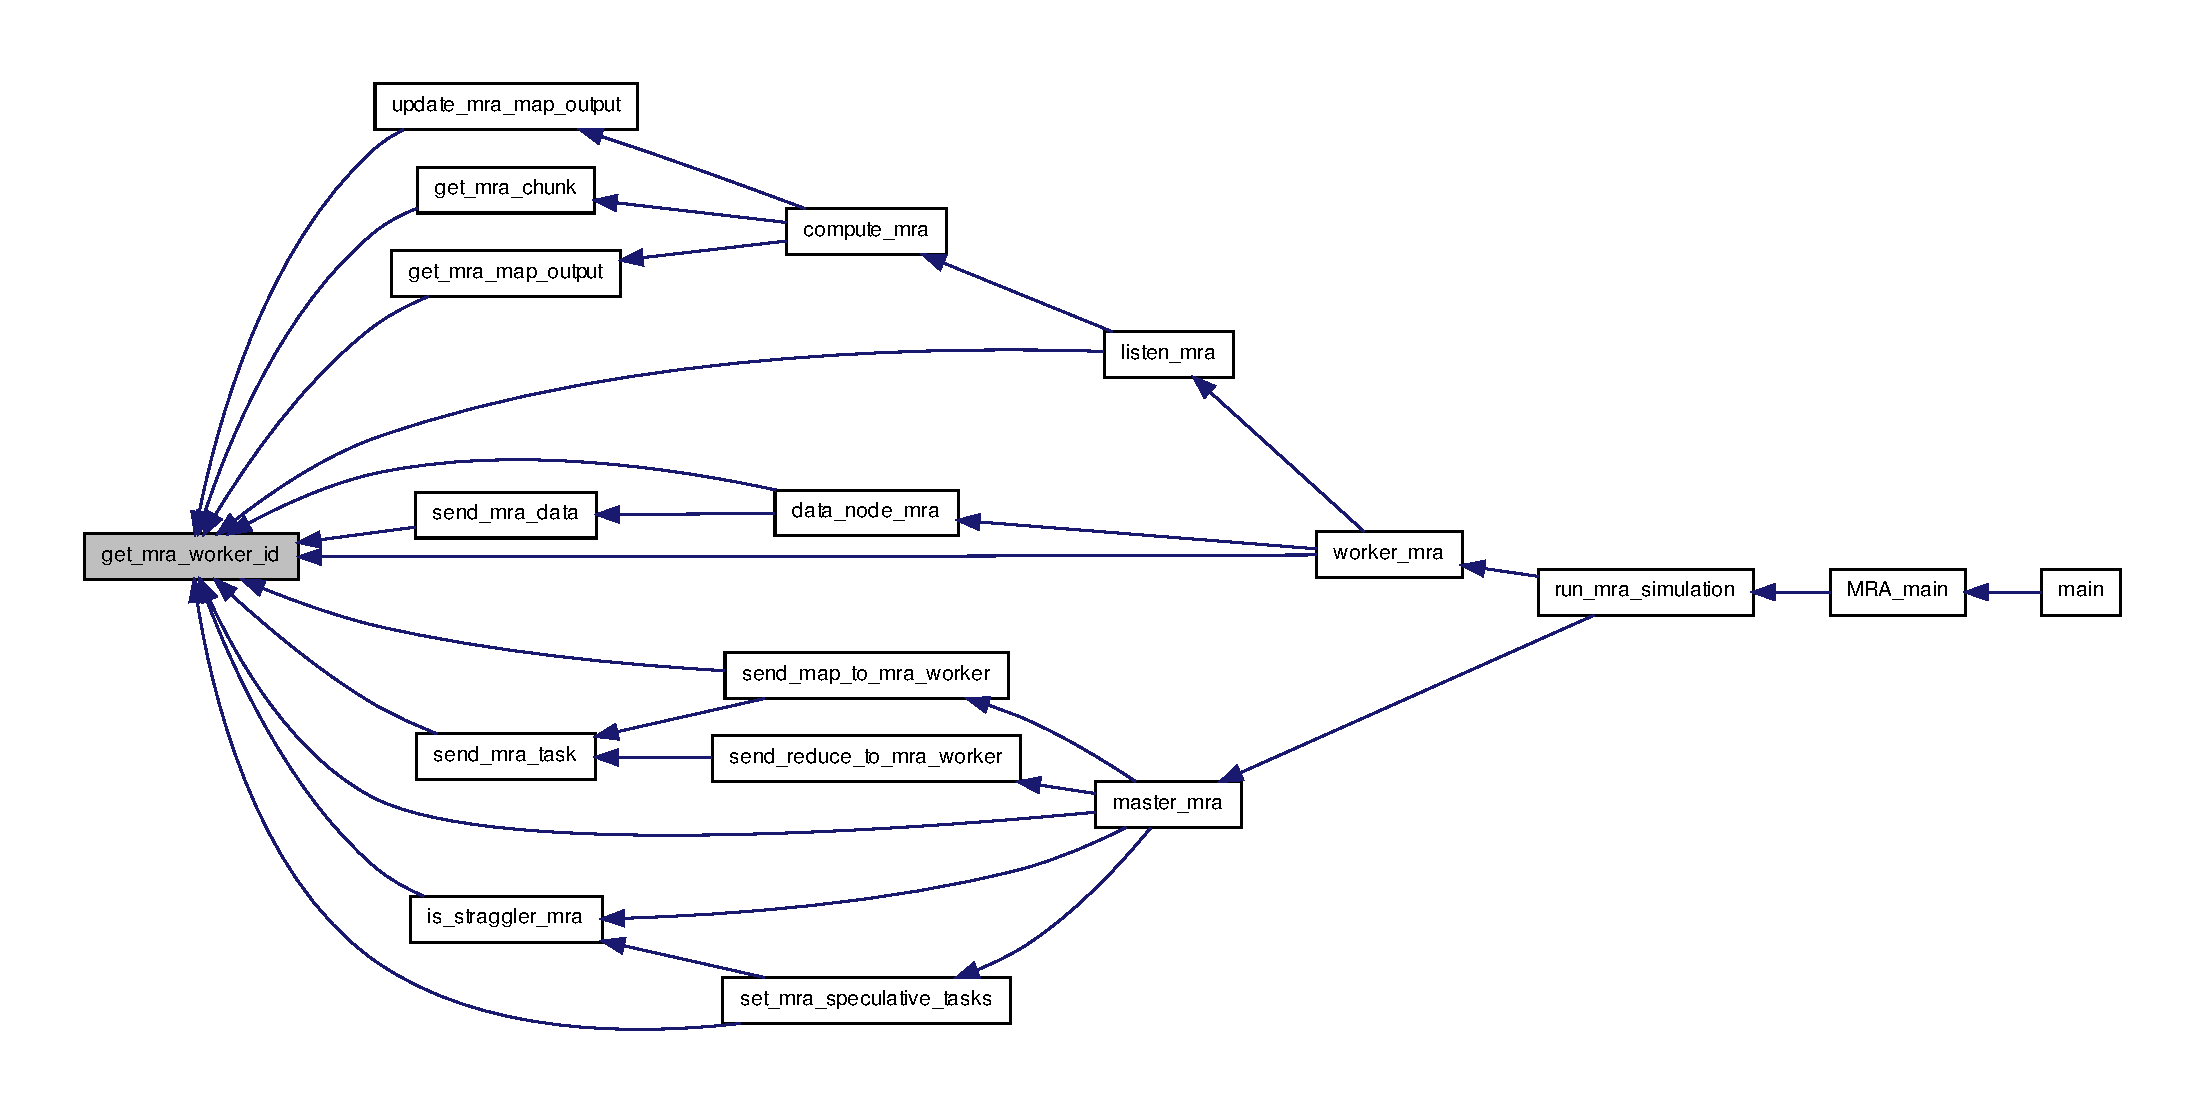
\includegraphics[width=350pt]{worker-mra_8h_a5c30e22e7fb9c6f78fca445efe8277f6_icgraph}
\end{center}
\end{figure}



\hypertarget{common-mra_8c}{\section{src/common-\/mra.c \-File \-Reference}
\label{common-mra_8c}\index{src/common-\/mra.\-c@{src/common-\/mra.\-c}}
}
{\ttfamily \#include \char`\"{}common-\/mra.\-h\char`\"{}}\*
\-Include dependency graph for common-\/mra.c\-:\nopagebreak
\begin{figure}[H]
\begin{center}
\leavevmode
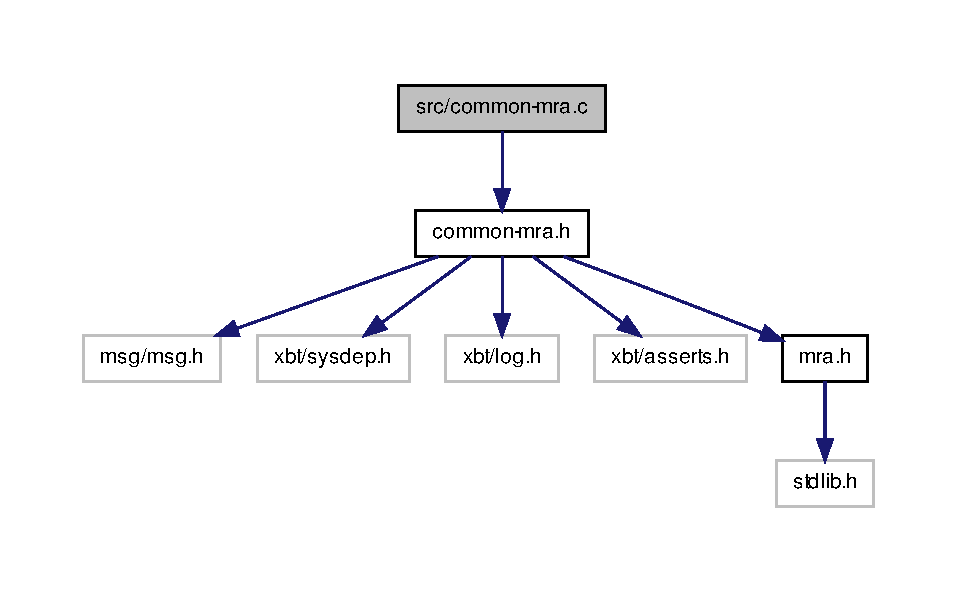
\includegraphics[width=350pt]{common-mra_8c__incl}
\end{center}
\end{figure}
\subsection*{\-Functions}
\begin{DoxyCompactItemize}
\item 
\hyperlink{common-mra_8c_a32bd1bae277b9aa336336310547bb693}{\-X\-B\-T\-\_\-\-L\-O\-G\-\_\-\-E\-X\-T\-E\-R\-N\-A\-L\-\_\-\-D\-E\-F\-A\-U\-L\-T\-\_\-\-C\-A\-T\-E\-G\-O\-R\-Y} (msg\-\_\-test)
\item 
msg\-\_\-error\-\_\-t \hyperlink{common-mra_8c_a385b12669d8faf7b5cdb54c1ae597e1c}{send} (const char $\ast$str, double cpu, double net, void $\ast$data, const char $\ast$mailbox)
\begin{DoxyCompactList}\small\item\em \-Send a message/task. \end{DoxyCompactList}\item 
msg\-\_\-error\-\_\-t \hyperlink{common-mra_8c_a305ac8e3389f94106990aa3c52c91416}{send\-\_\-mra\-\_\-sms} (const char $\ast$str, const char $\ast$mailbox)
\begin{DoxyCompactList}\small\item\em \-Send a short message, of size zero. \end{DoxyCompactList}\item 
msg\-\_\-error\-\_\-t \hyperlink{common-mra_8c_a6fc60933b9eabe64a880f68eba3131cc}{receive} (msg\-\_\-task\-\_\-t $\ast$msg, const char $\ast$mailbox)
\begin{DoxyCompactList}\small\item\em \-Receive a message/task from a mailbox. \end{DoxyCompactList}\item 
int \hyperlink{common-mra_8c_ad37a02c988c597622a346cb5293243fb}{message\-\_\-is} (msg\-\_\-task\-\_\-t msg, const char $\ast$str)
\begin{DoxyCompactList}\small\item\em \-Compare the message from a task with a string. \end{DoxyCompactList}\item 
int \hyperlink{common-mra_8c_a411d5133ab6881d40ef4cb44a7a47428}{maxval} (int a, int b)
\begin{DoxyCompactList}\small\item\em \-Return the maximum of two values. \end{DoxyCompactList}\item 
size\-\_\-t \hyperlink{common-mra_8c_a1df0d355a0754a40a7697437294d8431}{map\-\_\-mra\-\_\-output\-\_\-size} (size\-\_\-t mid)
\begin{DoxyCompactList}\small\item\em \-Return the output size of a map task. \end{DoxyCompactList}\item 
size\-\_\-t \hyperlink{common-mra_8c_a8205e98d4874b7e31f138d5016ad1eba}{reduce\-\_\-mra\-\_\-input\-\_\-size} (size\-\_\-t rid)
\begin{DoxyCompactList}\small\item\em \-Return the input size of a reduce task. \end{DoxyCompactList}\end{DoxyCompactItemize}


\subsection{\-Function \-Documentation}
\hypertarget{common-mra_8c_a1df0d355a0754a40a7697437294d8431}{\index{common-\/mra.\-c@{common-\/mra.\-c}!map\-\_\-mra\-\_\-output\-\_\-size@{map\-\_\-mra\-\_\-output\-\_\-size}}
\index{map\-\_\-mra\-\_\-output\-\_\-size@{map\-\_\-mra\-\_\-output\-\_\-size}!common-mra.c@{common-\/mra.\-c}}
\subsubsection[{map\-\_\-mra\-\_\-output\-\_\-size}]{\setlength{\rightskip}{0pt plus 5cm}size\-\_\-t {\bf map\-\_\-mra\-\_\-output\-\_\-size} (
\begin{DoxyParamCaption}
\item[{size\-\_\-t}]{mid}
\end{DoxyParamCaption}
)}}\label{common-mra_8c_a1df0d355a0754a40a7697437294d8431}


\-Return the output size of a map task. 


\begin{DoxyParams}{\-Parameters}
{\em mid} & \-The map task \-I\-D. \\
\hline
\end{DoxyParams}
\begin{DoxyReturn}{\-Returns}
\-The task output size in bytes. 
\end{DoxyReturn}
\hypertarget{common-mra_8c_a411d5133ab6881d40ef4cb44a7a47428}{\index{common-\/mra.\-c@{common-\/mra.\-c}!maxval@{maxval}}
\index{maxval@{maxval}!common-mra.c@{common-\/mra.\-c}}
\subsubsection[{maxval}]{\setlength{\rightskip}{0pt plus 5cm}int {\bf maxval} (
\begin{DoxyParamCaption}
\item[{int}]{a, }
\item[{int}]{b}
\end{DoxyParamCaption}
)}}\label{common-mra_8c_a411d5133ab6881d40ef4cb44a7a47428}


\-Return the maximum of two values. 



\-Here is the caller graph for this function\-:\nopagebreak
\begin{figure}[H]
\begin{center}
\leavevmode
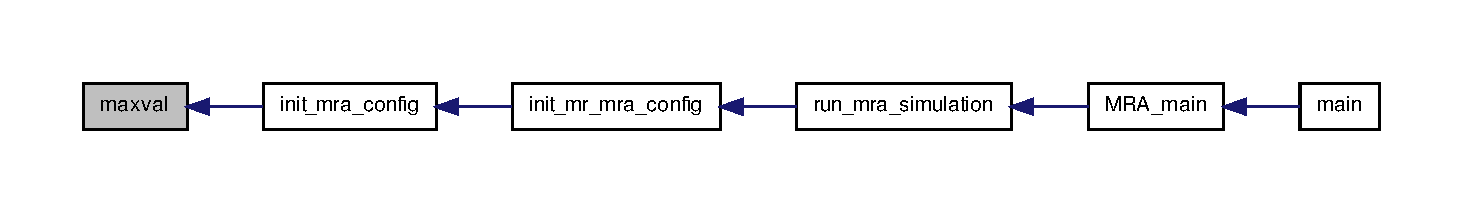
\includegraphics[width=350pt]{common-mra_8c_a411d5133ab6881d40ef4cb44a7a47428_icgraph}
\end{center}
\end{figure}


\hypertarget{common-mra_8c_ad37a02c988c597622a346cb5293243fb}{\index{common-\/mra.\-c@{common-\/mra.\-c}!message\-\_\-is@{message\-\_\-is}}
\index{message\-\_\-is@{message\-\_\-is}!common-mra.c@{common-\/mra.\-c}}
\subsubsection[{message\-\_\-is}]{\setlength{\rightskip}{0pt plus 5cm}int {\bf message\-\_\-is} (
\begin{DoxyParamCaption}
\item[{msg\-\_\-task\-\_\-t}]{msg, }
\item[{const char $\ast$}]{str}
\end{DoxyParamCaption}
)}}\label{common-mra_8c_ad37a02c988c597622a346cb5293243fb}


\-Compare the message from a task with a string. 


\begin{DoxyParams}{\-Parameters}
{\em msg} & \-The message/task. \\
\hline
{\em str} & \-The string to compare with. \\
\hline
\end{DoxyParams}
\begin{DoxyReturn}{\-Returns}
\-A positive value if matches, zero if doesn't. 
\end{DoxyReturn}


\-Here is the caller graph for this function\-:\nopagebreak
\begin{figure}[H]
\begin{center}
\leavevmode
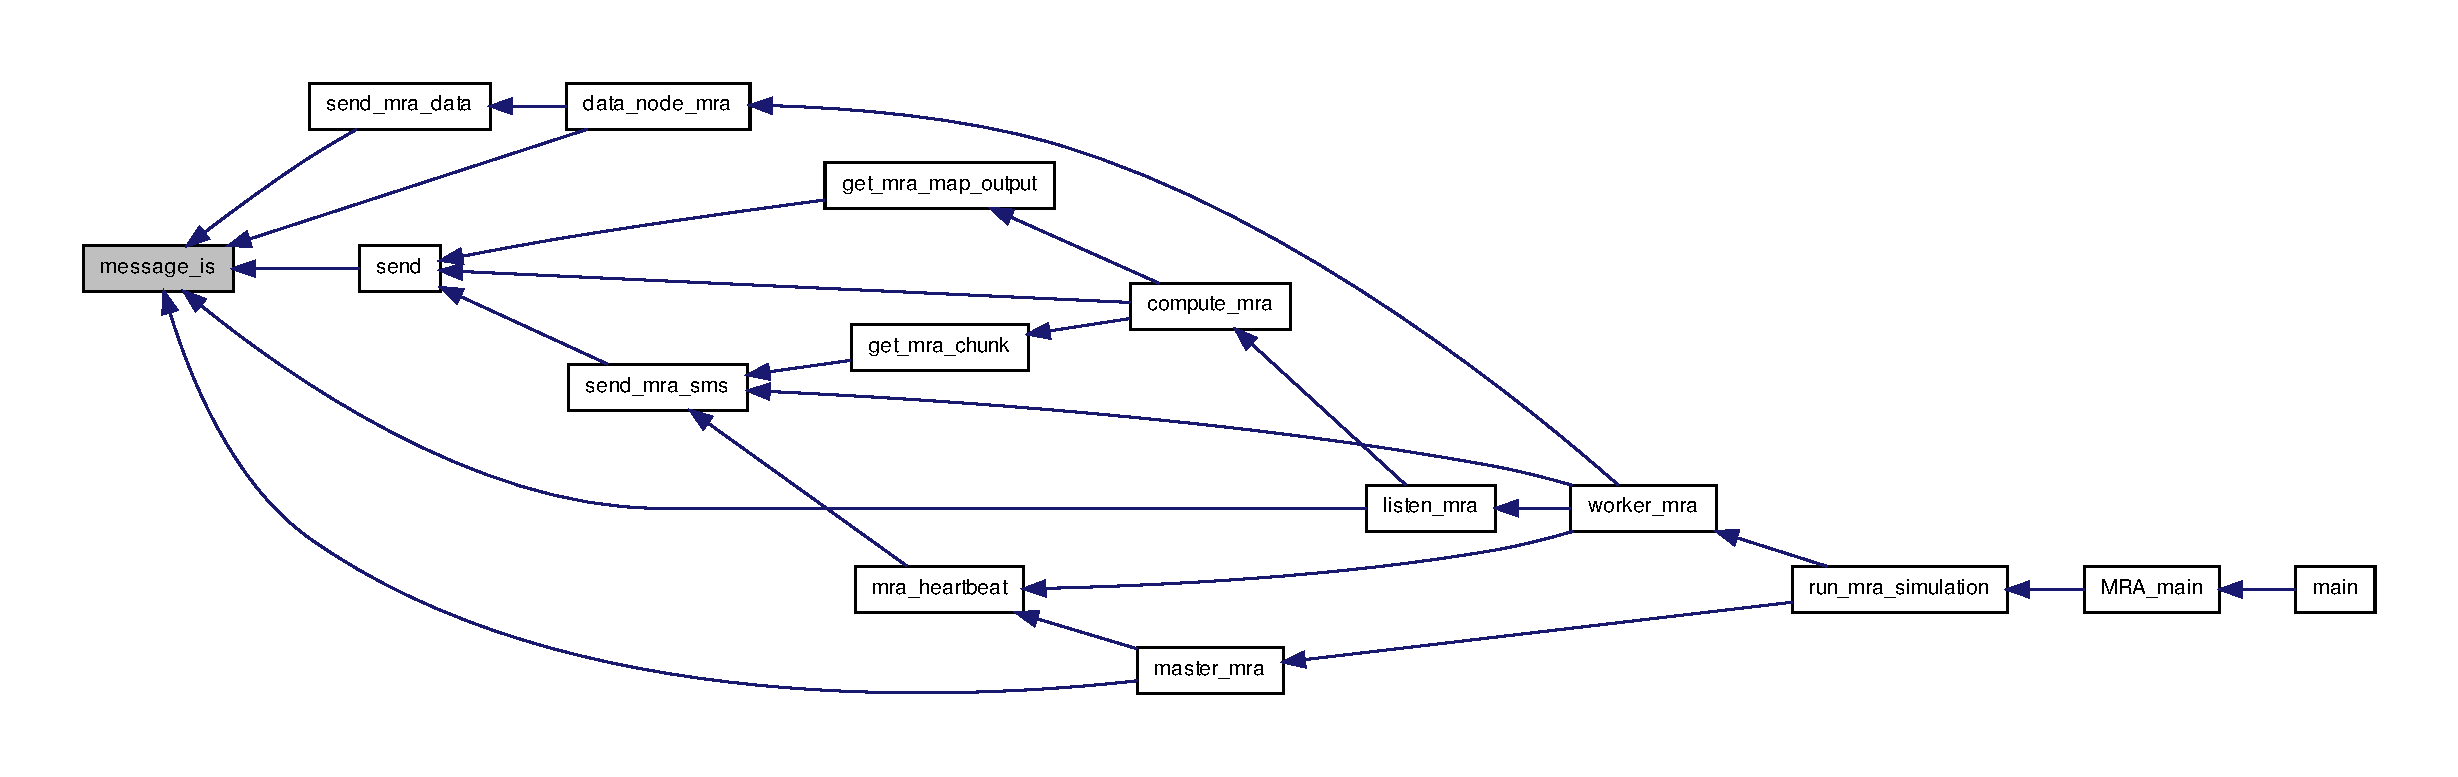
\includegraphics[width=350pt]{common-mra_8c_ad37a02c988c597622a346cb5293243fb_icgraph}
\end{center}
\end{figure}


\hypertarget{common-mra_8c_a6fc60933b9eabe64a880f68eba3131cc}{\index{common-\/mra.\-c@{common-\/mra.\-c}!receive@{receive}}
\index{receive@{receive}!common-mra.c@{common-\/mra.\-c}}
\subsubsection[{receive}]{\setlength{\rightskip}{0pt plus 5cm}msg\-\_\-error\-\_\-t {\bf receive} (
\begin{DoxyParamCaption}
\item[{msg\-\_\-task\-\_\-t $\ast$}]{msg, }
\item[{const char $\ast$}]{mailbox}
\end{DoxyParamCaption}
)}}\label{common-mra_8c_a6fc60933b9eabe64a880f68eba3131cc}


\-Receive a message/task from a mailbox. 


\begin{DoxyParams}{\-Parameters}
{\em msg} & \-Where to store the received message. \\
\hline
{\em mailbox} & \-The mailbox alias. \\
\hline
\end{DoxyParams}
\begin{DoxyReturn}{\-Returns}
\-The status of the transfer. 
\end{DoxyReturn}


\-Here is the caller graph for this function\-:\nopagebreak
\begin{figure}[H]
\begin{center}
\leavevmode
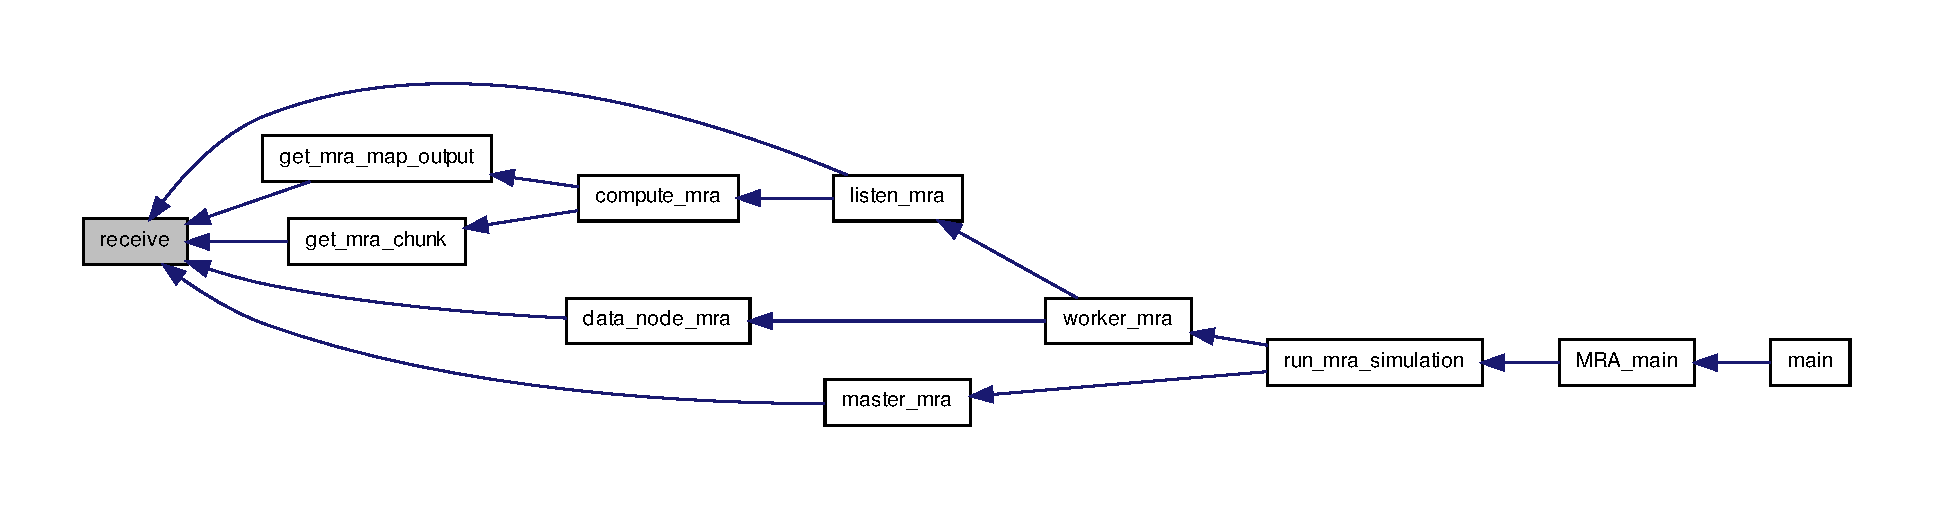
\includegraphics[width=350pt]{common-mra_8c_a6fc60933b9eabe64a880f68eba3131cc_icgraph}
\end{center}
\end{figure}


\hypertarget{common-mra_8c_a8205e98d4874b7e31f138d5016ad1eba}{\index{common-\/mra.\-c@{common-\/mra.\-c}!reduce\-\_\-mra\-\_\-input\-\_\-size@{reduce\-\_\-mra\-\_\-input\-\_\-size}}
\index{reduce\-\_\-mra\-\_\-input\-\_\-size@{reduce\-\_\-mra\-\_\-input\-\_\-size}!common-mra.c@{common-\/mra.\-c}}
\subsubsection[{reduce\-\_\-mra\-\_\-input\-\_\-size}]{\setlength{\rightskip}{0pt plus 5cm}size\-\_\-t {\bf reduce\-\_\-mra\-\_\-input\-\_\-size} (
\begin{DoxyParamCaption}
\item[{size\-\_\-t}]{rid}
\end{DoxyParamCaption}
)}}\label{common-mra_8c_a8205e98d4874b7e31f138d5016ad1eba}


\-Return the input size of a reduce task. 


\begin{DoxyParams}{\-Parameters}
{\em rid} & \-The reduce task \-I\-D. \\
\hline
\end{DoxyParams}
\begin{DoxyReturn}{\-Returns}
\-The task input size in bytes. 
\end{DoxyReturn}


\-Here is the caller graph for this function\-:\nopagebreak
\begin{figure}[H]
\begin{center}
\leavevmode
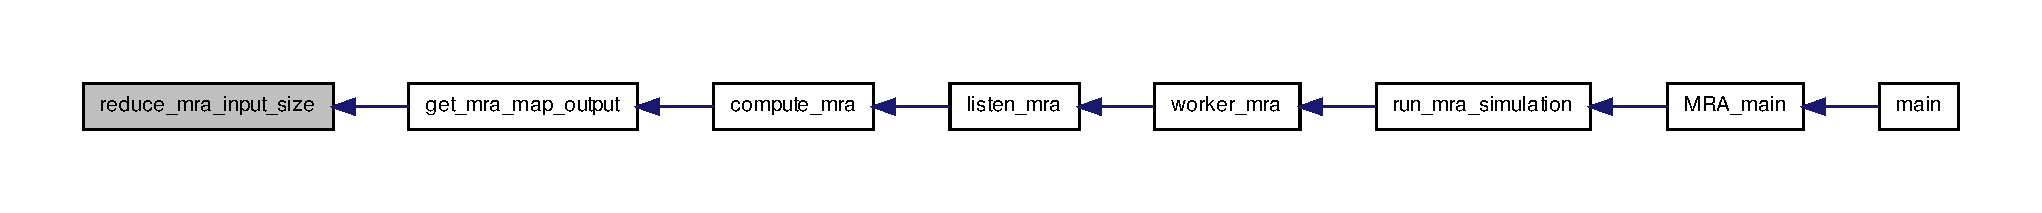
\includegraphics[width=350pt]{common-mra_8c_a8205e98d4874b7e31f138d5016ad1eba_icgraph}
\end{center}
\end{figure}


\hypertarget{common-mra_8c_a385b12669d8faf7b5cdb54c1ae597e1c}{\index{common-\/mra.\-c@{common-\/mra.\-c}!send@{send}}
\index{send@{send}!common-mra.c@{common-\/mra.\-c}}
\subsubsection[{send}]{\setlength{\rightskip}{0pt plus 5cm}msg\-\_\-error\-\_\-t {\bf send} (
\begin{DoxyParamCaption}
\item[{const char $\ast$}]{str, }
\item[{double}]{cpu, }
\item[{double}]{net, }
\item[{void $\ast$}]{data, }
\item[{const char $\ast$}]{mailbox}
\end{DoxyParamCaption}
)}}\label{common-mra_8c_a385b12669d8faf7b5cdb54c1ae597e1c}


\-Send a message/task. 


\begin{DoxyParams}{\-Parameters}
{\em str} & \-The message. \\
\hline
{\em cpu} & \-The amount of cpu required by the task. \\
\hline
{\em net} & \-The message size in bytes. \\
\hline
{\em data} & \-Any data to attatch to the message. \\
\hline
{\em mailbox} & \-The destination mailbox alias. \\
\hline
\end{DoxyParams}
\begin{DoxyReturn}{\-Returns}
\-The \-M\-S\-G status of the operation. 
\end{DoxyReturn}


\-Here is the call graph for this function\-:\nopagebreak
\begin{figure}[H]
\begin{center}
\leavevmode
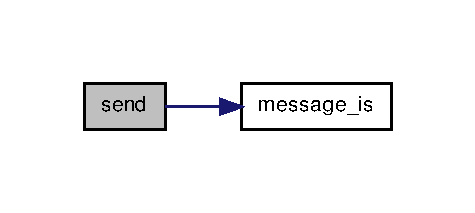
\includegraphics[width=228pt]{common-mra_8c_a385b12669d8faf7b5cdb54c1ae597e1c_cgraph}
\end{center}
\end{figure}




\-Here is the caller graph for this function\-:\nopagebreak
\begin{figure}[H]
\begin{center}
\leavevmode
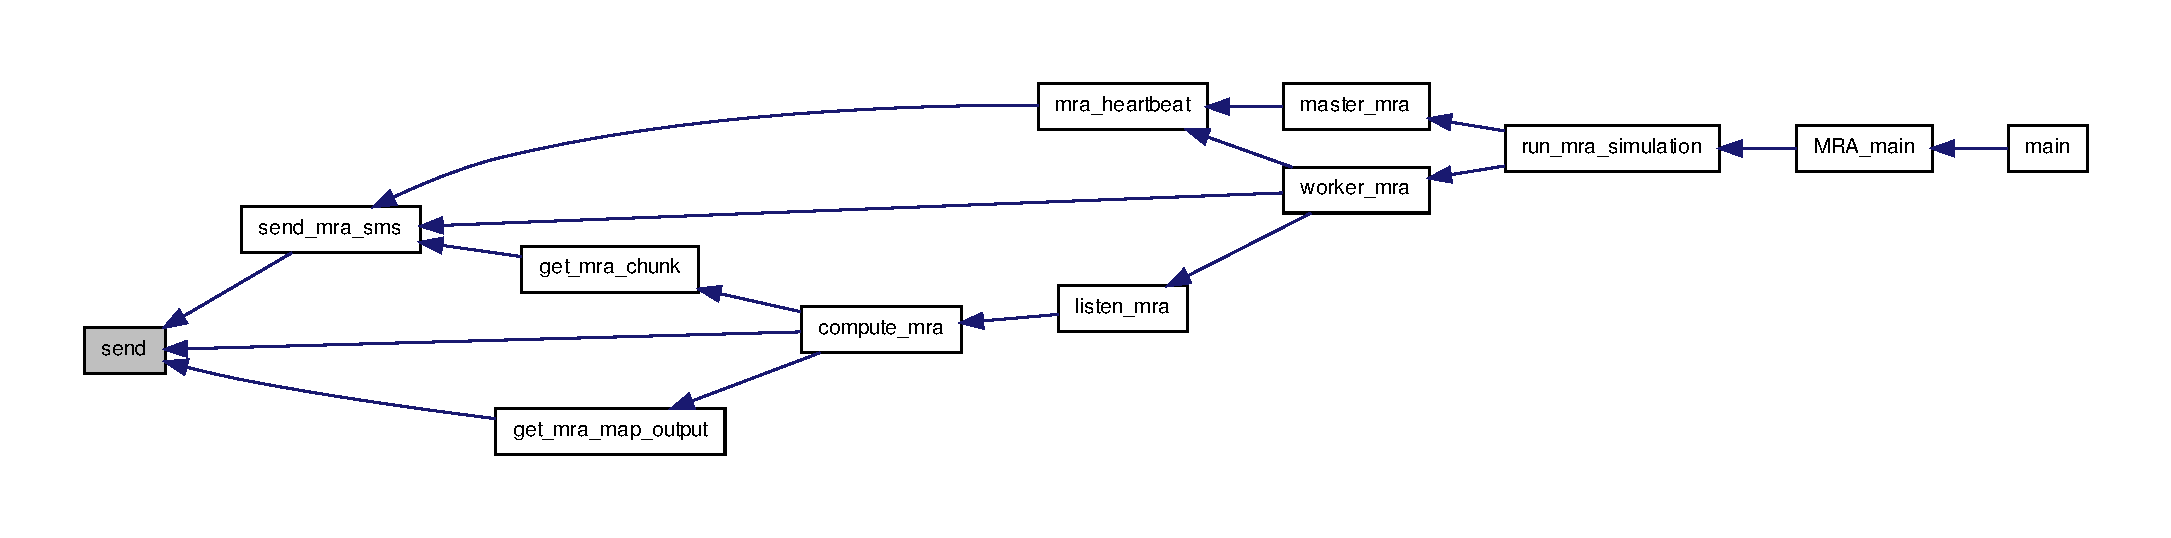
\includegraphics[width=350pt]{common-mra_8c_a385b12669d8faf7b5cdb54c1ae597e1c_icgraph}
\end{center}
\end{figure}


\hypertarget{common-mra_8c_a305ac8e3389f94106990aa3c52c91416}{\index{common-\/mra.\-c@{common-\/mra.\-c}!send\-\_\-mra\-\_\-sms@{send\-\_\-mra\-\_\-sms}}
\index{send\-\_\-mra\-\_\-sms@{send\-\_\-mra\-\_\-sms}!common-mra.c@{common-\/mra.\-c}}
\subsubsection[{send\-\_\-mra\-\_\-sms}]{\setlength{\rightskip}{0pt plus 5cm}msg\-\_\-error\-\_\-t {\bf send\-\_\-mra\-\_\-sms} (
\begin{DoxyParamCaption}
\item[{const char $\ast$}]{str, }
\item[{const char $\ast$}]{mailbox}
\end{DoxyParamCaption}
)}}\label{common-mra_8c_a305ac8e3389f94106990aa3c52c91416}


\-Send a short message, of size zero. 


\begin{DoxyParams}{\-Parameters}
{\em str} & \-The message. \\
\hline
{\em mailbox} & \-The destination mailbox alias. \\
\hline
\end{DoxyParams}
\begin{DoxyReturn}{\-Returns}
\-The \-M\-S\-G status of the operation. 
\end{DoxyReturn}


\-Here is the call graph for this function\-:\nopagebreak
\begin{figure}[H]
\begin{center}
\leavevmode
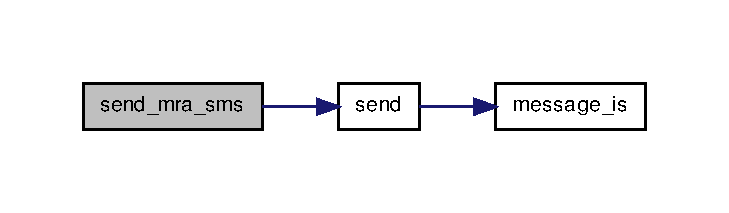
\includegraphics[width=350pt]{common-mra_8c_a305ac8e3389f94106990aa3c52c91416_cgraph}
\end{center}
\end{figure}




\-Here is the caller graph for this function\-:\nopagebreak
\begin{figure}[H]
\begin{center}
\leavevmode
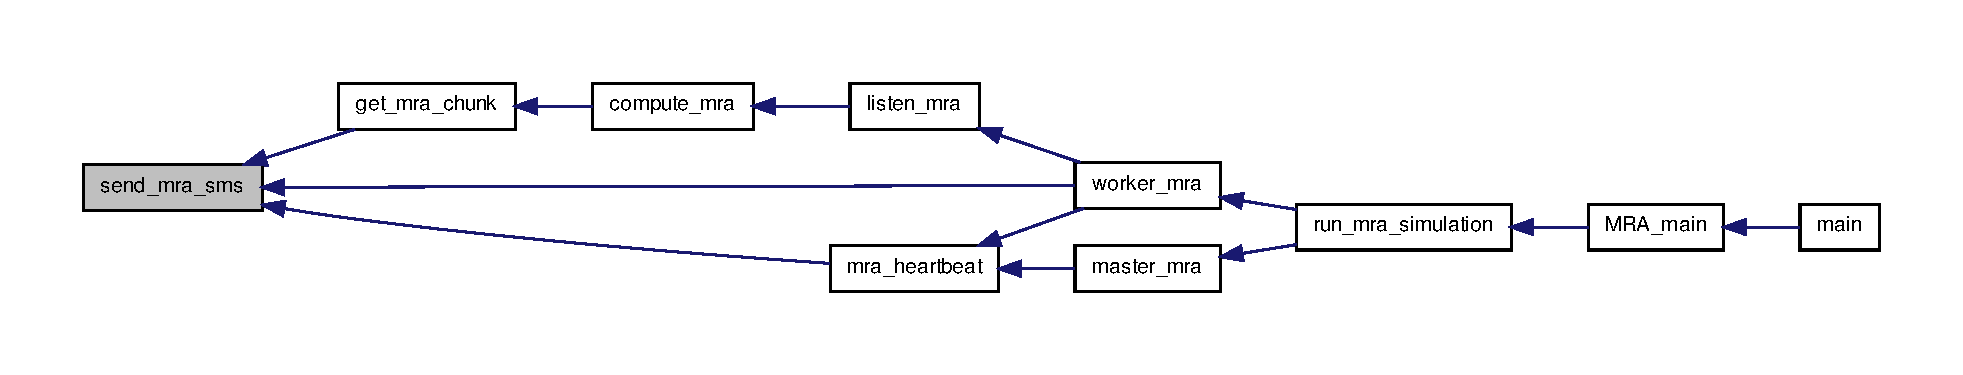
\includegraphics[width=350pt]{common-mra_8c_a305ac8e3389f94106990aa3c52c91416_icgraph}
\end{center}
\end{figure}


\hypertarget{common-mra_8c_a32bd1bae277b9aa336336310547bb693}{\index{common-\/mra.\-c@{common-\/mra.\-c}!\-X\-B\-T\-\_\-\-L\-O\-G\-\_\-\-E\-X\-T\-E\-R\-N\-A\-L\-\_\-\-D\-E\-F\-A\-U\-L\-T\-\_\-\-C\-A\-T\-E\-G\-O\-R\-Y@{\-X\-B\-T\-\_\-\-L\-O\-G\-\_\-\-E\-X\-T\-E\-R\-N\-A\-L\-\_\-\-D\-E\-F\-A\-U\-L\-T\-\_\-\-C\-A\-T\-E\-G\-O\-R\-Y}}
\index{\-X\-B\-T\-\_\-\-L\-O\-G\-\_\-\-E\-X\-T\-E\-R\-N\-A\-L\-\_\-\-D\-E\-F\-A\-U\-L\-T\-\_\-\-C\-A\-T\-E\-G\-O\-R\-Y@{\-X\-B\-T\-\_\-\-L\-O\-G\-\_\-\-E\-X\-T\-E\-R\-N\-A\-L\-\_\-\-D\-E\-F\-A\-U\-L\-T\-\_\-\-C\-A\-T\-E\-G\-O\-R\-Y}!common-mra.c@{common-\/mra.\-c}}
\subsubsection[{\-X\-B\-T\-\_\-\-L\-O\-G\-\_\-\-E\-X\-T\-E\-R\-N\-A\-L\-\_\-\-D\-E\-F\-A\-U\-L\-T\-\_\-\-C\-A\-T\-E\-G\-O\-R\-Y}]{\setlength{\rightskip}{0pt plus 5cm}{\bf \-X\-B\-T\-\_\-\-L\-O\-G\-\_\-\-E\-X\-T\-E\-R\-N\-A\-L\-\_\-\-D\-E\-F\-A\-U\-L\-T\-\_\-\-C\-A\-T\-E\-G\-O\-R\-Y} (
\begin{DoxyParamCaption}
\item[{msg\-\_\-test}]{}
\end{DoxyParamCaption}
)}}\label{common-mra_8c_a32bd1bae277b9aa336336310547bb693}

\hypertarget{dfs-mra_8c}{\section{src/dfs-\/mra.c \-File \-Reference}
\label{dfs-mra_8c}\index{src/dfs-\/mra.\-c@{src/dfs-\/mra.\-c}}
}
{\ttfamily \#include $<$math.\-h$>$}\*
{\ttfamily \#include $<$msg/msg.\-h$>$}\*
{\ttfamily \#include \char`\"{}common-\/mra.\-h\char`\"{}}\*
{\ttfamily \#include \char`\"{}worker-\/mra.\-h\char`\"{}}\*
{\ttfamily \#include \char`\"{}dfs-\/mra.\-h\char`\"{}}\*
\-Include dependency graph for dfs-\/mra.c\-:\nopagebreak
\begin{figure}[H]
\begin{center}
\leavevmode
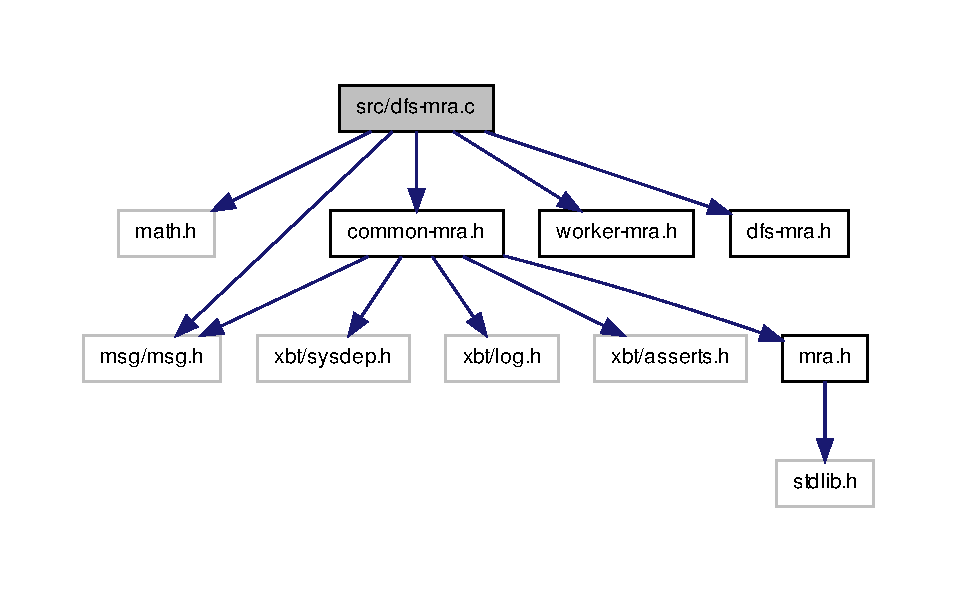
\includegraphics[width=350pt]{dfs-mra_8c__incl}
\end{center}
\end{figure}
\subsection*{\-Functions}
\begin{DoxyCompactItemize}
\item 
\hyperlink{dfs-mra_8c_a32bd1bae277b9aa336336310547bb693}{\-X\-B\-T\-\_\-\-L\-O\-G\-\_\-\-E\-X\-T\-E\-R\-N\-A\-L\-\_\-\-D\-E\-F\-A\-U\-L\-T\-\_\-\-C\-A\-T\-E\-G\-O\-R\-Y} (msg\-\_\-test)
\item 
static void \hyperlink{dfs-mra_8c_ada0444d4646937f1f59da2d5bd5cfad2}{send\-\_\-mra\-\_\-data} (msg\-\_\-task\-\_\-t msg)
\begin{DoxyCompactList}\small\item\em \-Process that responds to data requests. \end{DoxyCompactList}\item 
void \hyperlink{dfs-mra_8c_a23d972ed8df40ef6ff709f57e3944042}{distribute\-\_\-data\-\_\-mra} (void)
\begin{DoxyCompactList}\small\item\em \-Distribute chunks (and replicas) to \-Data\-Nodes. \end{DoxyCompactList}\item 
void \hyperlink{dfs-mra_8c_ac144b7da2b0cb2e76cf7226740c54dc1}{default\-\_\-mra\-\_\-dfs\-\_\-f} (char $\ast$$\ast$mra\-\_\-dfs\-\_\-matrix, size\-\_\-t chunks, size\-\_\-t workers\-\_\-mra, int replicas)
\begin{DoxyCompactList}\small\item\em \-Default data distribution algorithm. \end{DoxyCompactList}\item 
size\-\_\-t \hyperlink{dfs-mra_8c_a3f8eddb9dd6200115f7d88325537035e}{find\-\_\-random\-\_\-mra\-\_\-chunk\-\_\-owner} (int cid)
\begin{DoxyCompactList}\small\item\em \-Choose a random \-Data\-Node that owns a specific chunk. \end{DoxyCompactList}\item 
int \hyperlink{dfs-mra_8c_a86d9bef64a7e145c3e00de4e74e8d1c6}{data\-\_\-node\-\_\-mra} (int argc, char $\ast$argv\mbox{[}$\,$\mbox{]})
\begin{DoxyCompactList}\small\item\em \-Data\-Node main function. \end{DoxyCompactList}\end{DoxyCompactItemize}


\subsection{\-Function \-Documentation}
\hypertarget{dfs-mra_8c_a86d9bef64a7e145c3e00de4e74e8d1c6}{\index{dfs-\/mra.\-c@{dfs-\/mra.\-c}!data\-\_\-node\-\_\-mra@{data\-\_\-node\-\_\-mra}}
\index{data\-\_\-node\-\_\-mra@{data\-\_\-node\-\_\-mra}!dfs-mra.c@{dfs-\/mra.\-c}}
\subsubsection[{data\-\_\-node\-\_\-mra}]{\setlength{\rightskip}{0pt plus 5cm}int {\bf data\-\_\-node\-\_\-mra} (
\begin{DoxyParamCaption}
\item[{int}]{argc, }
\item[{char $\ast$}]{argv\mbox{[}$\,$\mbox{]}}
\end{DoxyParamCaption}
)}}\label{dfs-mra_8c_a86d9bef64a7e145c3e00de4e74e8d1c6}


\-Data\-Node main function. 

\-Process that listens for data requests. 

\-Here is the call graph for this function\-:\nopagebreak
\begin{figure}[H]
\begin{center}
\leavevmode
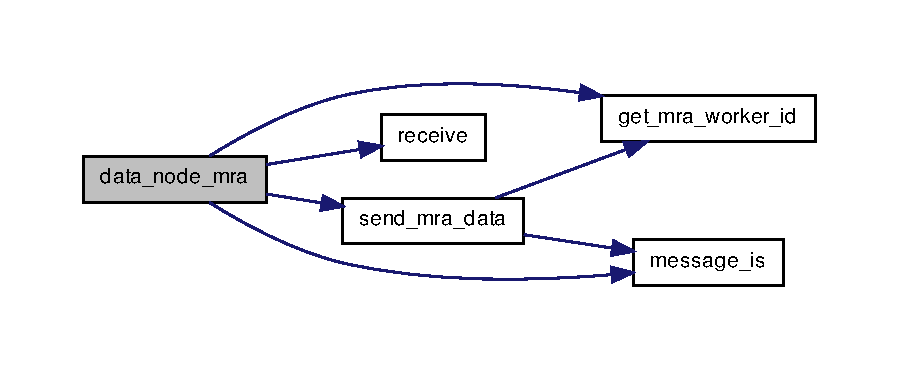
\includegraphics[width=350pt]{dfs-mra_8c_a86d9bef64a7e145c3e00de4e74e8d1c6_cgraph}
\end{center}
\end{figure}




\-Here is the caller graph for this function\-:\nopagebreak
\begin{figure}[H]
\begin{center}
\leavevmode
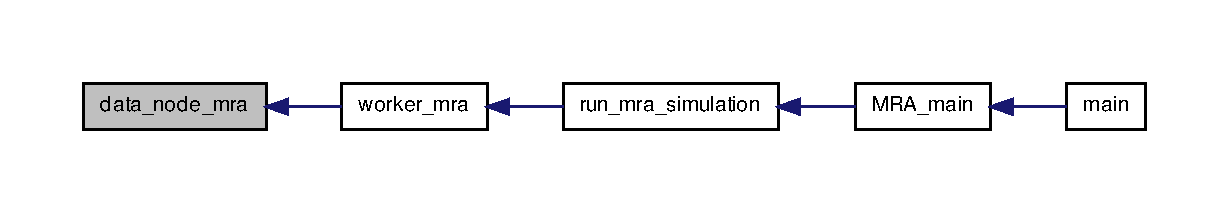
\includegraphics[width=350pt]{dfs-mra_8c_a86d9bef64a7e145c3e00de4e74e8d1c6_icgraph}
\end{center}
\end{figure}


\hypertarget{dfs-mra_8c_ac144b7da2b0cb2e76cf7226740c54dc1}{\index{dfs-\/mra.\-c@{dfs-\/mra.\-c}!default\-\_\-mra\-\_\-dfs\-\_\-f@{default\-\_\-mra\-\_\-dfs\-\_\-f}}
\index{default\-\_\-mra\-\_\-dfs\-\_\-f@{default\-\_\-mra\-\_\-dfs\-\_\-f}!dfs-mra.c@{dfs-\/mra.\-c}}
\subsubsection[{default\-\_\-mra\-\_\-dfs\-\_\-f}]{\setlength{\rightskip}{0pt plus 5cm}void {\bf default\-\_\-mra\-\_\-dfs\-\_\-f} (
\begin{DoxyParamCaption}
\item[{char $\ast$$\ast$}]{mra\-\_\-dfs\-\_\-matrix, }
\item[{size\-\_\-t}]{chunks, }
\item[{size\-\_\-t}]{workers\-\_\-mra, }
\item[{int}]{replicas}
\end{DoxyParamCaption}
)}}\label{dfs-mra_8c_ac144b7da2b0cb2e76cf7226740c54dc1}


\-Default data distribution algorithm. 

de workers -\/-\/$>$ workers\-\_\-hosts\mbox{[}id\mbox{]} (array)  capacidade -\/-\/$>$ \-M\-S\-G\-\_\-get\-\_\-host\-\_\-speed (config\-\_\-mra.\-workers\mbox{[}owner\mbox{]})  -\/-\/$>$ \-Calcula a capacidade computacional relativa de cada worker baseado na capacidade total da grid.  -\/-\/$>$ É o array com as tribuições brutas, antes do ajuste de menor te\-\_\-exec  -\/-\/$>$ É o array com o valor de previsão de término de todas as tarefas distribuídas ao worker;  -\/-\/$>$ É o array com o tempo que será utilizado para encontar a melhor distribuição  -\/-\/$>$ É o array que contém o tempo de cada worker para executar uma tarefa computacional padrão

config\-\_\-mra.\-slots\-\_\-mra\mbox{[}\-M\-R\-A\-\_\-\-M\-A\-P\mbox{]};

-\/-\/$>$ verifica qual é o maior tempo de execução previsto

\-Ajuste de \-Força \-Bruta com uma \-Otimização \-Combinatória para obter uma distribuição de chunks com o menor tempo de execução possível

\-Here is the caller graph for this function\-:\nopagebreak
\begin{figure}[H]
\begin{center}
\leavevmode
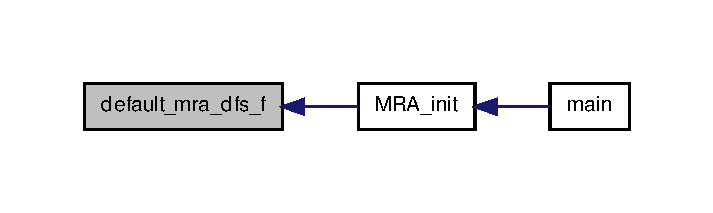
\includegraphics[width=342pt]{dfs-mra_8c_ac144b7da2b0cb2e76cf7226740c54dc1_icgraph}
\end{center}
\end{figure}


\hypertarget{dfs-mra_8c_a23d972ed8df40ef6ff709f57e3944042}{\index{dfs-\/mra.\-c@{dfs-\/mra.\-c}!distribute\-\_\-data\-\_\-mra@{distribute\-\_\-data\-\_\-mra}}
\index{distribute\-\_\-data\-\_\-mra@{distribute\-\_\-data\-\_\-mra}!dfs-mra.c@{dfs-\/mra.\-c}}
\subsubsection[{distribute\-\_\-data\-\_\-mra}]{\setlength{\rightskip}{0pt plus 5cm}void {\bf distribute\-\_\-data\-\_\-mra} (
\begin{DoxyParamCaption}
\item[{void}]{}
\end{DoxyParamCaption}
)}}\label{dfs-mra_8c_a23d972ed8df40ef6ff709f57e3944042}


\-Distribute chunks (and replicas) to \-Data\-Nodes. 



\-Here is the caller graph for this function\-:\nopagebreak
\begin{figure}[H]
\begin{center}
\leavevmode
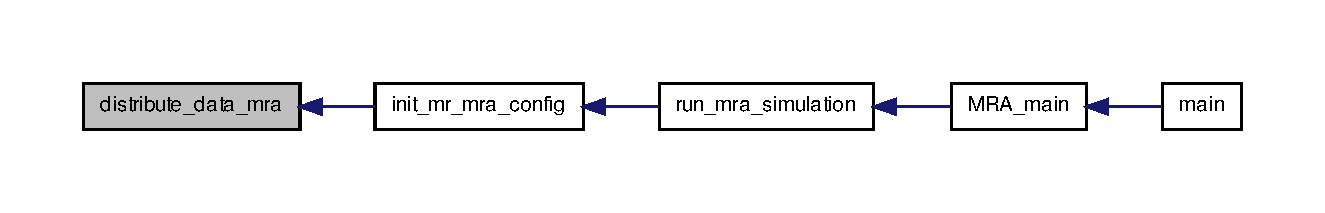
\includegraphics[width=350pt]{dfs-mra_8c_a23d972ed8df40ef6ff709f57e3944042_icgraph}
\end{center}
\end{figure}


\hypertarget{dfs-mra_8c_a3f8eddb9dd6200115f7d88325537035e}{\index{dfs-\/mra.\-c@{dfs-\/mra.\-c}!find\-\_\-random\-\_\-mra\-\_\-chunk\-\_\-owner@{find\-\_\-random\-\_\-mra\-\_\-chunk\-\_\-owner}}
\index{find\-\_\-random\-\_\-mra\-\_\-chunk\-\_\-owner@{find\-\_\-random\-\_\-mra\-\_\-chunk\-\_\-owner}!dfs-mra.c@{dfs-\/mra.\-c}}
\subsubsection[{find\-\_\-random\-\_\-mra\-\_\-chunk\-\_\-owner}]{\setlength{\rightskip}{0pt plus 5cm}size\-\_\-t {\bf find\-\_\-random\-\_\-mra\-\_\-chunk\-\_\-owner} (
\begin{DoxyParamCaption}
\item[{int}]{cid}
\end{DoxyParamCaption}
)}}\label{dfs-mra_8c_a3f8eddb9dd6200115f7d88325537035e}


\-Choose a random \-Data\-Node that owns a specific chunk. 

\-Distribution of \-Data \-Replication 
\begin{DoxyParams}{\-Parameters}
{\em cid} & \-The chunk \-I\-D. \\
\hline
\end{DoxyParams}
\begin{DoxyReturn}{\-Returns}
\-The \-I\-D of the \-Data\-Node. 
\end{DoxyReturn}


\-Here is the caller graph for this function\-:\nopagebreak
\begin{figure}[H]
\begin{center}
\leavevmode
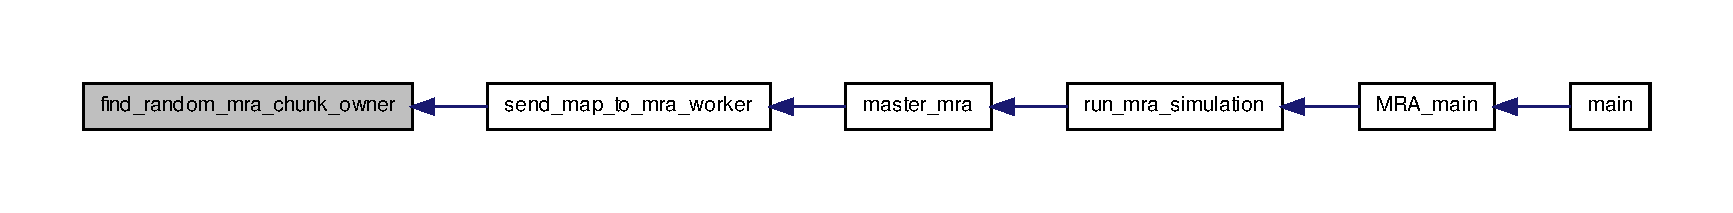
\includegraphics[width=350pt]{dfs-mra_8c_a3f8eddb9dd6200115f7d88325537035e_icgraph}
\end{center}
\end{figure}


\hypertarget{dfs-mra_8c_ada0444d4646937f1f59da2d5bd5cfad2}{\index{dfs-\/mra.\-c@{dfs-\/mra.\-c}!send\-\_\-mra\-\_\-data@{send\-\_\-mra\-\_\-data}}
\index{send\-\_\-mra\-\_\-data@{send\-\_\-mra\-\_\-data}!dfs-mra.c@{dfs-\/mra.\-c}}
\subsubsection[{send\-\_\-mra\-\_\-data}]{\setlength{\rightskip}{0pt plus 5cm}static void {\bf send\-\_\-mra\-\_\-data} (
\begin{DoxyParamCaption}
\item[{msg\-\_\-task\-\_\-t}]{msg}
\end{DoxyParamCaption}
)\hspace{0.3cm}{\ttfamily  \mbox{[}static\mbox{]}}}}\label{dfs-mra_8c_ada0444d4646937f1f59da2d5bd5cfad2}


\-Process that responds to data requests. 



\-Here is the call graph for this function\-:\nopagebreak
\begin{figure}[H]
\begin{center}
\leavevmode
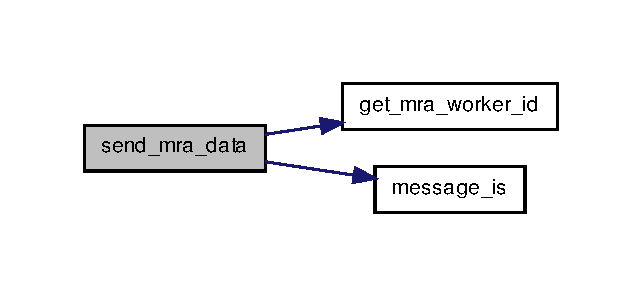
\includegraphics[width=308pt]{dfs-mra_8c_ada0444d4646937f1f59da2d5bd5cfad2_cgraph}
\end{center}
\end{figure}




\-Here is the caller graph for this function\-:\nopagebreak
\begin{figure}[H]
\begin{center}
\leavevmode
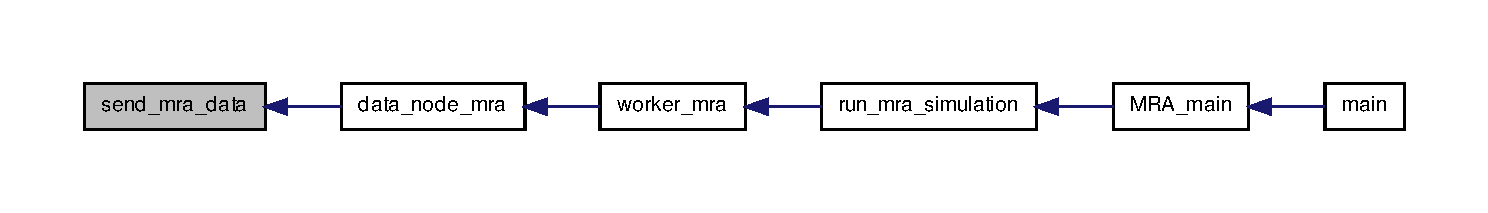
\includegraphics[width=350pt]{dfs-mra_8c_ada0444d4646937f1f59da2d5bd5cfad2_icgraph}
\end{center}
\end{figure}


\hypertarget{dfs-mra_8c_a32bd1bae277b9aa336336310547bb693}{\index{dfs-\/mra.\-c@{dfs-\/mra.\-c}!\-X\-B\-T\-\_\-\-L\-O\-G\-\_\-\-E\-X\-T\-E\-R\-N\-A\-L\-\_\-\-D\-E\-F\-A\-U\-L\-T\-\_\-\-C\-A\-T\-E\-G\-O\-R\-Y@{\-X\-B\-T\-\_\-\-L\-O\-G\-\_\-\-E\-X\-T\-E\-R\-N\-A\-L\-\_\-\-D\-E\-F\-A\-U\-L\-T\-\_\-\-C\-A\-T\-E\-G\-O\-R\-Y}}
\index{\-X\-B\-T\-\_\-\-L\-O\-G\-\_\-\-E\-X\-T\-E\-R\-N\-A\-L\-\_\-\-D\-E\-F\-A\-U\-L\-T\-\_\-\-C\-A\-T\-E\-G\-O\-R\-Y@{\-X\-B\-T\-\_\-\-L\-O\-G\-\_\-\-E\-X\-T\-E\-R\-N\-A\-L\-\_\-\-D\-E\-F\-A\-U\-L\-T\-\_\-\-C\-A\-T\-E\-G\-O\-R\-Y}!dfs-mra.c@{dfs-\/mra.\-c}}
\subsubsection[{\-X\-B\-T\-\_\-\-L\-O\-G\-\_\-\-E\-X\-T\-E\-R\-N\-A\-L\-\_\-\-D\-E\-F\-A\-U\-L\-T\-\_\-\-C\-A\-T\-E\-G\-O\-R\-Y}]{\setlength{\rightskip}{0pt plus 5cm}{\bf \-X\-B\-T\-\_\-\-L\-O\-G\-\_\-\-E\-X\-T\-E\-R\-N\-A\-L\-\_\-\-D\-E\-F\-A\-U\-L\-T\-\_\-\-C\-A\-T\-E\-G\-O\-R\-Y} (
\begin{DoxyParamCaption}
\item[{msg\-\_\-test}]{}
\end{DoxyParamCaption}
)}}\label{dfs-mra_8c_a32bd1bae277b9aa336336310547bb693}

\hypertarget{master-mra_8c}{\section{src/master-\/mra.c \-File \-Reference}
\label{master-mra_8c}\index{src/master-\/mra.\-c@{src/master-\/mra.\-c}}
}
{\ttfamily \#include $<$stdlib.\-h$>$}\*
{\ttfamily \#include $<$stdio.\-h$>$}\*
{\ttfamily \#include $<$string.\-h$>$}\*
{\ttfamily \#include \char`\"{}common-\/mra.\-h\char`\"{}}\*
{\ttfamily \#include \char`\"{}worker-\/mra.\-h\char`\"{}}\*
{\ttfamily \#include \char`\"{}dfs-\/mra.\-h\char`\"{}}\*
\-Include dependency graph for master-\/mra.c\-:\nopagebreak
\begin{figure}[H]
\begin{center}
\leavevmode
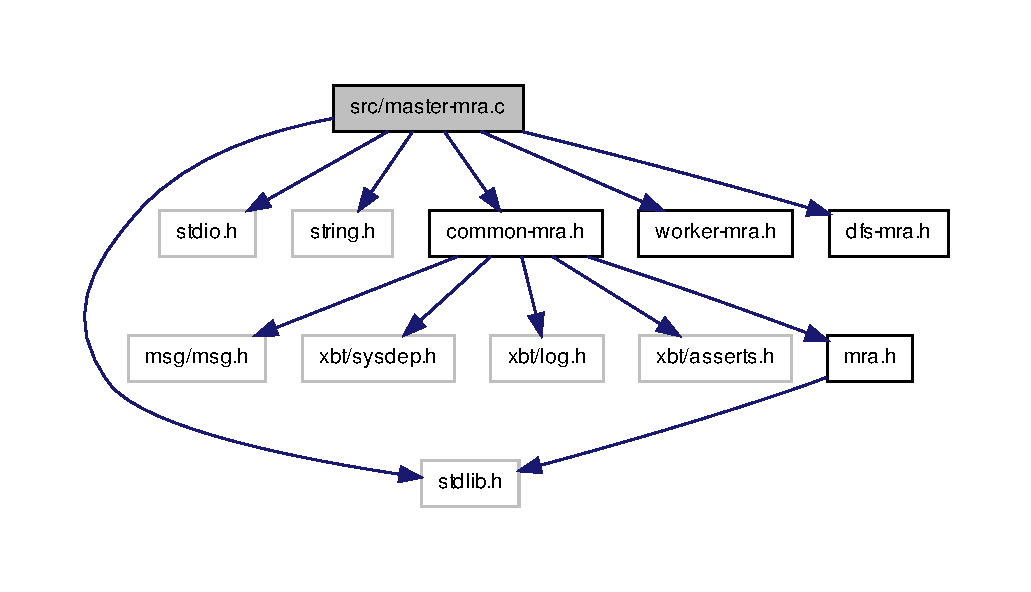
\includegraphics[width=350pt]{master-mra_8c__incl}
\end{center}
\end{figure}
\subsection*{\-Functions}
\begin{DoxyCompactItemize}
\item 
\hyperlink{master-mra_8c_a32bd1bae277b9aa336336310547bb693}{\-X\-B\-T\-\_\-\-L\-O\-G\-\_\-\-E\-X\-T\-E\-R\-N\-A\-L\-\_\-\-D\-E\-F\-A\-U\-L\-T\-\_\-\-C\-A\-T\-E\-G\-O\-R\-Y} (msg\-\_\-test)
\item 
static void \hyperlink{master-mra_8c_a35e18876ff26f7fe749fe4aeba3a7208}{print\-\_\-mra\-\_\-config} (void)
\begin{DoxyCompactList}\small\item\em \-Print the job configuration. \end{DoxyCompactList}\item 
static void \hyperlink{master-mra_8c_ad10e64f15346eb21a4a4b2dab5ab4007}{print\-\_\-mra\-\_\-stats} (void)
\begin{DoxyCompactList}\small\item\em \-Print job statistics. \end{DoxyCompactList}\item 
static int \hyperlink{master-mra_8c_a31c4fbd19a29ede1d95f2b70901f0670}{is\-\_\-straggler\-\_\-mra} (enum \hyperlink{mra_8h_afa14b6e068c0e0b8557777e16f2582f2}{phase\-\_\-e} phase, msg\-\_\-host\-\_\-t worker)
\begin{DoxyCompactList}\small\item\em \-Checks if a worker is a straggler. \end{DoxyCompactList}\item 
static int \hyperlink{master-mra_8c_a307706539b3d6ddd301c250ef7e0990c}{task\-\_\-time\-\_\-elapsed\-\_\-mra} (msg\-\_\-task\-\_\-t task)
\begin{DoxyCompactList}\small\item\em \-Returns for how long a task is running. \end{DoxyCompactList}\item 
static void \hyperlink{master-mra_8c_a769bac1cdfdfc862a1c9dc5444a47c95}{set\-\_\-mra\-\_\-speculative\-\_\-tasks} (enum \hyperlink{mra_8h_afa14b6e068c0e0b8557777e16f2582f2}{phase\-\_\-e} phase, msg\-\_\-host\-\_\-t worker)
\begin{DoxyCompactList}\small\item\em \-Mark the tasks of a straggler as possible speculative tasks. \end{DoxyCompactList}\item 
static void \hyperlink{master-mra_8c_a54a5360a29540b0302528bf7c22af577}{send\-\_\-map\-\_\-to\-\_\-mra\-\_\-worker} (msg\-\_\-host\-\_\-t dest)
\begin{DoxyCompactList}\small\item\em \-Choose a map task, and send it to a worker. \end{DoxyCompactList}\item 
static void \hyperlink{master-mra_8c_a11c1ba3e81b04f147dddbfcc637ffd1f}{send\-\_\-reduce\-\_\-to\-\_\-mra\-\_\-worker} (msg\-\_\-host\-\_\-t dest)
\begin{DoxyCompactList}\small\item\em \-Choose a reduce task, and send it to a worker. \end{DoxyCompactList}\item 
static void \hyperlink{master-mra_8c_ad1217d5b8cdd99a1e7b3755a9761d4ee}{send\-\_\-mra\-\_\-task} (enum \hyperlink{mra_8h_afa14b6e068c0e0b8557777e16f2582f2}{phase\-\_\-e} phase, size\-\_\-t tid, size\-\_\-t data\-\_\-src, msg\-\_\-host\-\_\-t dest)
\begin{DoxyCompactList}\small\item\em \-Send a task to a worker. \end{DoxyCompactList}\item 
static void \hyperlink{master-mra_8c_abb91a100f0067b79a6d171ee510df540}{finish\-\_\-all\-\_\-mra\-\_\-task\-\_\-copies} (\hyperlink{common-mra_8h_a54f41524090023e9b283ecbef8b955d6}{mra\-\_\-task\-\_\-info\-\_\-t} ti)
\begin{DoxyCompactList}\small\item\em \-Kill all copies of a task. \end{DoxyCompactList}\item 
int \hyperlink{master-mra_8c_afc38789b94eade9a7b1c6ae97a784af1}{master\-\_\-mra} (int argc, char $\ast$argv\mbox{[}$\,$\mbox{]})
\begin{DoxyCompactList}\small\item\em \-Main master function. \end{DoxyCompactList}\end{DoxyCompactItemize}
\subsection*{\-Variables}
\begin{DoxyCompactItemize}
\item 
static \-F\-I\-L\-E $\ast$ \hyperlink{master-mra_8c_a42ff89a9ffd23ba410ff217181554f6c}{tasks\-\_\-log}
\end{DoxyCompactItemize}


\subsection{\-Function \-Documentation}
\hypertarget{master-mra_8c_abb91a100f0067b79a6d171ee510df540}{\index{master-\/mra.\-c@{master-\/mra.\-c}!finish\-\_\-all\-\_\-mra\-\_\-task\-\_\-copies@{finish\-\_\-all\-\_\-mra\-\_\-task\-\_\-copies}}
\index{finish\-\_\-all\-\_\-mra\-\_\-task\-\_\-copies@{finish\-\_\-all\-\_\-mra\-\_\-task\-\_\-copies}!master-mra.c@{master-\/mra.\-c}}
\subsubsection[{finish\-\_\-all\-\_\-mra\-\_\-task\-\_\-copies}]{\setlength{\rightskip}{0pt plus 5cm}static void {\bf finish\-\_\-all\-\_\-mra\-\_\-task\-\_\-copies} (
\begin{DoxyParamCaption}
\item[{{\bf mra\-\_\-task\-\_\-info\-\_\-t}}]{ti}
\end{DoxyParamCaption}
)\hspace{0.3cm}{\ttfamily  \mbox{[}static\mbox{]}}}}\label{master-mra_8c_abb91a100f0067b79a6d171ee510df540}


\-Kill all copies of a task. 


\begin{DoxyParams}{\-Parameters}
{\em ti} & \-The task information of any task instance. \\
\hline
\end{DoxyParams}


\-Here is the caller graph for this function\-:\nopagebreak
\begin{figure}[H]
\begin{center}
\leavevmode
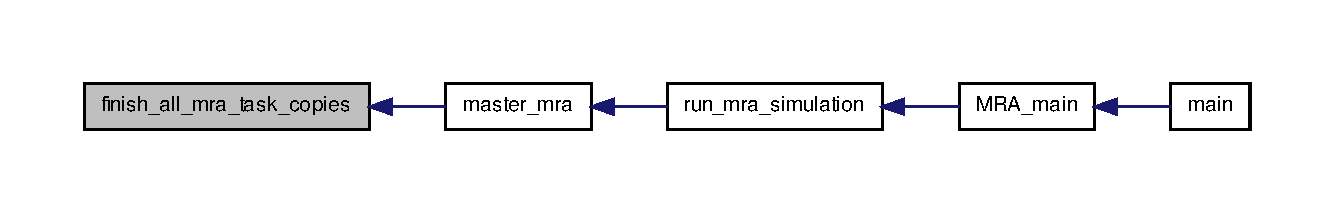
\includegraphics[width=350pt]{master-mra_8c_abb91a100f0067b79a6d171ee510df540_icgraph}
\end{center}
\end{figure}


\hypertarget{master-mra_8c_a31c4fbd19a29ede1d95f2b70901f0670}{\index{master-\/mra.\-c@{master-\/mra.\-c}!is\-\_\-straggler\-\_\-mra@{is\-\_\-straggler\-\_\-mra}}
\index{is\-\_\-straggler\-\_\-mra@{is\-\_\-straggler\-\_\-mra}!master-mra.c@{master-\/mra.\-c}}
\subsubsection[{is\-\_\-straggler\-\_\-mra}]{\setlength{\rightskip}{0pt plus 5cm}static int {\bf is\-\_\-straggler\-\_\-mra} (
\begin{DoxyParamCaption}
\item[{enum {\bf phase\-\_\-e}}]{phase, }
\item[{msg\-\_\-host\-\_\-t}]{worker}
\end{DoxyParamCaption}
)\hspace{0.3cm}{\ttfamily  \mbox{[}static\mbox{]}}}}\label{master-mra_8c_a31c4fbd19a29ede1d95f2b70901f0670}


\-Checks if a worker is a straggler. 


\begin{DoxyParams}{\-Parameters}
{\em worker} & \-The worker to be probed. \\
\hline
\end{DoxyParams}
\begin{DoxyReturn}{\-Returns}
1 if true, 0 if false. 
\end{DoxyReturn}


\-Here is the call graph for this function\-:\nopagebreak
\begin{figure}[H]
\begin{center}
\leavevmode
\includegraphics[width=312pt]{master-mra_8c_a31c4fbd19a29ede1d95f2b70901f0670_cgraph}
\end{center}
\end{figure}




\-Here is the caller graph for this function\-:\nopagebreak
\begin{figure}[H]
\begin{center}
\leavevmode
\includegraphics[width=350pt]{master-mra_8c_a31c4fbd19a29ede1d95f2b70901f0670_icgraph}
\end{center}
\end{figure}


\hypertarget{master-mra_8c_afc38789b94eade9a7b1c6ae97a784af1}{\index{master-\/mra.\-c@{master-\/mra.\-c}!master\-\_\-mra@{master\-\_\-mra}}
\index{master\-\_\-mra@{master\-\_\-mra}!master-mra.c@{master-\/mra.\-c}}
\subsubsection[{master\-\_\-mra}]{\setlength{\rightskip}{0pt plus 5cm}int {\bf master\-\_\-mra} (
\begin{DoxyParamCaption}
\item[{int}]{argc, }
\item[{char $\ast$}]{argv\mbox{[}$\,$\mbox{]}}
\end{DoxyParamCaption}
)}}\label{master-mra_8c_afc38789b94eade9a7b1c6ae97a784af1}


\-Main master function. 



\-Here is the call graph for this function\-:\nopagebreak
\begin{figure}[H]
\begin{center}
\leavevmode
\includegraphics[width=350pt]{master-mra_8c_afc38789b94eade9a7b1c6ae97a784af1_cgraph}
\end{center}
\end{figure}




\-Here is the caller graph for this function\-:\nopagebreak
\begin{figure}[H]
\begin{center}
\leavevmode
\includegraphics[width=350pt]{master-mra_8c_afc38789b94eade9a7b1c6ae97a784af1_icgraph}
\end{center}
\end{figure}


\hypertarget{master-mra_8c_a35e18876ff26f7fe749fe4aeba3a7208}{\index{master-\/mra.\-c@{master-\/mra.\-c}!print\-\_\-mra\-\_\-config@{print\-\_\-mra\-\_\-config}}
\index{print\-\_\-mra\-\_\-config@{print\-\_\-mra\-\_\-config}!master-mra.c@{master-\/mra.\-c}}
\subsubsection[{print\-\_\-mra\-\_\-config}]{\setlength{\rightskip}{0pt plus 5cm}static void {\bf print\-\_\-mra\-\_\-config} (
\begin{DoxyParamCaption}
\item[{void}]{}
\end{DoxyParamCaption}
)\hspace{0.3cm}{\ttfamily  \mbox{[}static\mbox{]}}}}\label{master-mra_8c_a35e18876ff26f7fe749fe4aeba3a7208}


\-Print the job configuration. 



\-Here is the caller graph for this function\-:\nopagebreak
\begin{figure}[H]
\begin{center}
\leavevmode
\includegraphics[width=350pt]{master-mra_8c_a35e18876ff26f7fe749fe4aeba3a7208_icgraph}
\end{center}
\end{figure}


\hypertarget{master-mra_8c_ad10e64f15346eb21a4a4b2dab5ab4007}{\index{master-\/mra.\-c@{master-\/mra.\-c}!print\-\_\-mra\-\_\-stats@{print\-\_\-mra\-\_\-stats}}
\index{print\-\_\-mra\-\_\-stats@{print\-\_\-mra\-\_\-stats}!master-mra.c@{master-\/mra.\-c}}
\subsubsection[{print\-\_\-mra\-\_\-stats}]{\setlength{\rightskip}{0pt plus 5cm}static void {\bf print\-\_\-mra\-\_\-stats} (
\begin{DoxyParamCaption}
\item[{void}]{}
\end{DoxyParamCaption}
)\hspace{0.3cm}{\ttfamily  \mbox{[}static\mbox{]}}}}\label{master-mra_8c_ad10e64f15346eb21a4a4b2dab5ab4007}


\-Print job statistics. 



\-Here is the caller graph for this function\-:\nopagebreak
\begin{figure}[H]
\begin{center}
\leavevmode
\includegraphics[width=350pt]{master-mra_8c_ad10e64f15346eb21a4a4b2dab5ab4007_icgraph}
\end{center}
\end{figure}


\hypertarget{master-mra_8c_a54a5360a29540b0302528bf7c22af577}{\index{master-\/mra.\-c@{master-\/mra.\-c}!send\-\_\-map\-\_\-to\-\_\-mra\-\_\-worker@{send\-\_\-map\-\_\-to\-\_\-mra\-\_\-worker}}
\index{send\-\_\-map\-\_\-to\-\_\-mra\-\_\-worker@{send\-\_\-map\-\_\-to\-\_\-mra\-\_\-worker}!master-mra.c@{master-\/mra.\-c}}
\subsubsection[{send\-\_\-map\-\_\-to\-\_\-mra\-\_\-worker}]{\setlength{\rightskip}{0pt plus 5cm}static void {\bf send\-\_\-map\-\_\-to\-\_\-mra\-\_\-worker} (
\begin{DoxyParamCaption}
\item[{msg\-\_\-host\-\_\-t}]{dest}
\end{DoxyParamCaption}
)\hspace{0.3cm}{\ttfamily  \mbox{[}static\mbox{]}}}}\label{master-mra_8c_a54a5360a29540b0302528bf7c22af577}


\-Choose a map task, and send it to a worker. 


\begin{DoxyParams}{\-Parameters}
{\em dest} & \-The destination worker. \\
\hline
\end{DoxyParams}


\-Here is the call graph for this function\-:\nopagebreak
\begin{figure}[H]
\begin{center}
\leavevmode
\includegraphics[width=350pt]{master-mra_8c_a54a5360a29540b0302528bf7c22af577_cgraph}
\end{center}
\end{figure}




\-Here is the caller graph for this function\-:\nopagebreak
\begin{figure}[H]
\begin{center}
\leavevmode
\includegraphics[width=350pt]{master-mra_8c_a54a5360a29540b0302528bf7c22af577_icgraph}
\end{center}
\end{figure}


\hypertarget{master-mra_8c_ad1217d5b8cdd99a1e7b3755a9761d4ee}{\index{master-\/mra.\-c@{master-\/mra.\-c}!send\-\_\-mra\-\_\-task@{send\-\_\-mra\-\_\-task}}
\index{send\-\_\-mra\-\_\-task@{send\-\_\-mra\-\_\-task}!master-mra.c@{master-\/mra.\-c}}
\subsubsection[{send\-\_\-mra\-\_\-task}]{\setlength{\rightskip}{0pt plus 5cm}static void {\bf send\-\_\-mra\-\_\-task} (
\begin{DoxyParamCaption}
\item[{enum {\bf phase\-\_\-e}}]{phase, }
\item[{size\-\_\-t}]{tid, }
\item[{size\-\_\-t}]{data\-\_\-src, }
\item[{msg\-\_\-host\-\_\-t}]{dest}
\end{DoxyParamCaption}
)\hspace{0.3cm}{\ttfamily  \mbox{[}static\mbox{]}}}}\label{master-mra_8c_ad1217d5b8cdd99a1e7b3755a9761d4ee}


\-Send a task to a worker. 


\begin{DoxyParams}{\-Parameters}
{\em phase} & \-The current job phase. \\
\hline
{\em tid} & \-The task \-I\-D. \\
\hline
{\em data\-\_\-src} & \-The \-I\-D of the \-Data\-Node that owns the task data. \\
\hline
{\em dest} & \-The destination worker. \\
\hline
\end{DoxyParams}


\-Here is the call graph for this function\-:\nopagebreak
\begin{figure}[H]
\begin{center}
\leavevmode
\includegraphics[width=306pt]{master-mra_8c_ad1217d5b8cdd99a1e7b3755a9761d4ee_cgraph}
\end{center}
\end{figure}




\-Here is the caller graph for this function\-:\nopagebreak
\begin{figure}[H]
\begin{center}
\leavevmode
\includegraphics[width=350pt]{master-mra_8c_ad1217d5b8cdd99a1e7b3755a9761d4ee_icgraph}
\end{center}
\end{figure}


\hypertarget{master-mra_8c_a11c1ba3e81b04f147dddbfcc637ffd1f}{\index{master-\/mra.\-c@{master-\/mra.\-c}!send\-\_\-reduce\-\_\-to\-\_\-mra\-\_\-worker@{send\-\_\-reduce\-\_\-to\-\_\-mra\-\_\-worker}}
\index{send\-\_\-reduce\-\_\-to\-\_\-mra\-\_\-worker@{send\-\_\-reduce\-\_\-to\-\_\-mra\-\_\-worker}!master-mra.c@{master-\/mra.\-c}}
\subsubsection[{send\-\_\-reduce\-\_\-to\-\_\-mra\-\_\-worker}]{\setlength{\rightskip}{0pt plus 5cm}static void {\bf send\-\_\-reduce\-\_\-to\-\_\-mra\-\_\-worker} (
\begin{DoxyParamCaption}
\item[{msg\-\_\-host\-\_\-t}]{dest}
\end{DoxyParamCaption}
)\hspace{0.3cm}{\ttfamily  \mbox{[}static\mbox{]}}}}\label{master-mra_8c_a11c1ba3e81b04f147dddbfcc637ffd1f}


\-Choose a reduce task, and send it to a worker. 


\begin{DoxyParams}{\-Parameters}
{\em dest} & \-The destination worker. \\
\hline
\end{DoxyParams}


\-Here is the call graph for this function\-:\nopagebreak
\begin{figure}[H]
\begin{center}
\leavevmode
\includegraphics[width=350pt]{master-mra_8c_a11c1ba3e81b04f147dddbfcc637ffd1f_cgraph}
\end{center}
\end{figure}




\-Here is the caller graph for this function\-:\nopagebreak
\begin{figure}[H]
\begin{center}
\leavevmode
\includegraphics[width=350pt]{master-mra_8c_a11c1ba3e81b04f147dddbfcc637ffd1f_icgraph}
\end{center}
\end{figure}


\hypertarget{master-mra_8c_a769bac1cdfdfc862a1c9dc5444a47c95}{\index{master-\/mra.\-c@{master-\/mra.\-c}!set\-\_\-mra\-\_\-speculative\-\_\-tasks@{set\-\_\-mra\-\_\-speculative\-\_\-tasks}}
\index{set\-\_\-mra\-\_\-speculative\-\_\-tasks@{set\-\_\-mra\-\_\-speculative\-\_\-tasks}!master-mra.c@{master-\/mra.\-c}}
\subsubsection[{set\-\_\-mra\-\_\-speculative\-\_\-tasks}]{\setlength{\rightskip}{0pt plus 5cm}static void {\bf set\-\_\-mra\-\_\-speculative\-\_\-tasks} (
\begin{DoxyParamCaption}
\item[{enum {\bf phase\-\_\-e}}]{phase, }
\item[{msg\-\_\-host\-\_\-t}]{worker}
\end{DoxyParamCaption}
)\hspace{0.3cm}{\ttfamily  \mbox{[}static\mbox{]}}}}\label{master-mra_8c_a769bac1cdfdfc862a1c9dc5444a47c95}


\-Mark the tasks of a straggler as possible speculative tasks. 


\begin{DoxyParams}{\-Parameters}
{\em worker} & \-The straggler worker. \\
\hline
\end{DoxyParams}


\-Here is the call graph for this function\-:\nopagebreak
\begin{figure}[H]
\begin{center}
\leavevmode
\includegraphics[width=350pt]{master-mra_8c_a769bac1cdfdfc862a1c9dc5444a47c95_cgraph}
\end{center}
\end{figure}




\-Here is the caller graph for this function\-:\nopagebreak
\begin{figure}[H]
\begin{center}
\leavevmode
\includegraphics[width=350pt]{master-mra_8c_a769bac1cdfdfc862a1c9dc5444a47c95_icgraph}
\end{center}
\end{figure}


\hypertarget{master-mra_8c_a307706539b3d6ddd301c250ef7e0990c}{\index{master-\/mra.\-c@{master-\/mra.\-c}!task\-\_\-time\-\_\-elapsed\-\_\-mra@{task\-\_\-time\-\_\-elapsed\-\_\-mra}}
\index{task\-\_\-time\-\_\-elapsed\-\_\-mra@{task\-\_\-time\-\_\-elapsed\-\_\-mra}!master-mra.c@{master-\/mra.\-c}}
\subsubsection[{task\-\_\-time\-\_\-elapsed\-\_\-mra}]{\setlength{\rightskip}{0pt plus 5cm}static int {\bf task\-\_\-time\-\_\-elapsed\-\_\-mra} (
\begin{DoxyParamCaption}
\item[{msg\-\_\-task\-\_\-t}]{task}
\end{DoxyParamCaption}
)\hspace{0.3cm}{\ttfamily  \mbox{[}static\mbox{]}}}}\label{master-mra_8c_a307706539b3d6ddd301c250ef7e0990c}


\-Returns for how long a task is running. 


\begin{DoxyParams}{\-Parameters}
{\em task} & \-The task to be probed. \\
\hline
\end{DoxyParams}
\begin{DoxyReturn}{\-Returns}
\-The amount of seconds since the beginning of the computation. 
\end{DoxyReturn}


\-Here is the caller graph for this function\-:\nopagebreak
\begin{figure}[H]
\begin{center}
\leavevmode
\includegraphics[width=350pt]{master-mra_8c_a307706539b3d6ddd301c250ef7e0990c_icgraph}
\end{center}
\end{figure}


\hypertarget{master-mra_8c_a32bd1bae277b9aa336336310547bb693}{\index{master-\/mra.\-c@{master-\/mra.\-c}!\-X\-B\-T\-\_\-\-L\-O\-G\-\_\-\-E\-X\-T\-E\-R\-N\-A\-L\-\_\-\-D\-E\-F\-A\-U\-L\-T\-\_\-\-C\-A\-T\-E\-G\-O\-R\-Y@{\-X\-B\-T\-\_\-\-L\-O\-G\-\_\-\-E\-X\-T\-E\-R\-N\-A\-L\-\_\-\-D\-E\-F\-A\-U\-L\-T\-\_\-\-C\-A\-T\-E\-G\-O\-R\-Y}}
\index{\-X\-B\-T\-\_\-\-L\-O\-G\-\_\-\-E\-X\-T\-E\-R\-N\-A\-L\-\_\-\-D\-E\-F\-A\-U\-L\-T\-\_\-\-C\-A\-T\-E\-G\-O\-R\-Y@{\-X\-B\-T\-\_\-\-L\-O\-G\-\_\-\-E\-X\-T\-E\-R\-N\-A\-L\-\_\-\-D\-E\-F\-A\-U\-L\-T\-\_\-\-C\-A\-T\-E\-G\-O\-R\-Y}!master-mra.c@{master-\/mra.\-c}}
\subsubsection[{\-X\-B\-T\-\_\-\-L\-O\-G\-\_\-\-E\-X\-T\-E\-R\-N\-A\-L\-\_\-\-D\-E\-F\-A\-U\-L\-T\-\_\-\-C\-A\-T\-E\-G\-O\-R\-Y}]{\setlength{\rightskip}{0pt plus 5cm}{\bf \-X\-B\-T\-\_\-\-L\-O\-G\-\_\-\-E\-X\-T\-E\-R\-N\-A\-L\-\_\-\-D\-E\-F\-A\-U\-L\-T\-\_\-\-C\-A\-T\-E\-G\-O\-R\-Y} (
\begin{DoxyParamCaption}
\item[{msg\-\_\-test}]{}
\end{DoxyParamCaption}
)}}\label{master-mra_8c_a32bd1bae277b9aa336336310547bb693}


\subsection{\-Variable \-Documentation}
\hypertarget{master-mra_8c_a42ff89a9ffd23ba410ff217181554f6c}{\index{master-\/mra.\-c@{master-\/mra.\-c}!tasks\-\_\-log@{tasks\-\_\-log}}
\index{tasks\-\_\-log@{tasks\-\_\-log}!master-mra.c@{master-\/mra.\-c}}
\subsubsection[{tasks\-\_\-log}]{\setlength{\rightskip}{0pt plus 5cm}\-F\-I\-L\-E$\ast$ {\bf tasks\-\_\-log}\hspace{0.3cm}{\ttfamily  \mbox{[}static\mbox{]}}}}\label{master-mra_8c_a42ff89a9ffd23ba410ff217181554f6c}

\hypertarget{simcore-mra_8c}{\section{src/simcore-\/mra.c \-File \-Reference}
\label{simcore-mra_8c}\index{src/simcore-\/mra.\-c@{src/simcore-\/mra.\-c}}
}
{\ttfamily \#include $<$msg/msg.\-h$>$}\*
{\ttfamily \#include $<$xbt/sysdep.\-h$>$}\*
{\ttfamily \#include $<$xbt/log.\-h$>$}\*
{\ttfamily \#include $<$xbt/asserts.\-h$>$}\*
{\ttfamily \#include \char`\"{}common-\/mra.\-h\char`\"{}}\*
{\ttfamily \#include \char`\"{}worker-\/mra.\-h\char`\"{}}\*
{\ttfamily \#include \char`\"{}dfs-\/mra.\-h\char`\"{}}\*
{\ttfamily \#include \char`\"{}mra.\-h\char`\"{}}\*
\-Include dependency graph for simcore-\/mra.c\-:\nopagebreak
\begin{figure}[H]
\begin{center}
\leavevmode
\includegraphics[width=350pt]{simcore-mra_8c__incl}
\end{center}
\end{figure}
\subsection*{\-Defines}
\begin{DoxyCompactItemize}
\item 
\#define \hyperlink{simcore-mra_8c_a706068f562dd5c64a8b7bbd4b2298dd1}{\-M\-A\-X\-\_\-\-L\-I\-N\-E\-\_\-\-S\-I\-Z\-E}~256
\end{DoxyCompactItemize}
\subsection*{\-Functions}
\begin{DoxyCompactItemize}
\item 
\hyperlink{simcore-mra_8c_ad2e657250a9756c87c6da2ea76f38875}{\-X\-B\-T\-\_\-\-L\-O\-G\-\_\-\-N\-E\-W\-\_\-\-D\-E\-F\-A\-U\-L\-T\-\_\-\-C\-A\-T\-E\-G\-O\-R\-Y} (msg\-\_\-test,\char`\"{}\-M\-R\-A\char`\"{})
\item 
int \hyperlink{simcore-mra_8c_afc38789b94eade9a7b1c6ae97a784af1}{master\-\_\-mra} (int argc, char $\ast$argv\mbox{[}$\,$\mbox{]})
\begin{DoxyCompactList}\small\item\em \-Main master function. \end{DoxyCompactList}\item 
int \hyperlink{simcore-mra_8c_a3f18ef8503f272839fc15596ace82344}{worker\-\_\-mra} (int argc, char $\ast$argv\mbox{[}$\,$\mbox{]})
\begin{DoxyCompactList}\small\item\em \-Main worker function. \end{DoxyCompactList}\item 
static void \hyperlink{simcore-mra_8c_a926867fcb6aaa2dcdd4f4a7ea5607a59}{check\-\_\-config\-\_\-mra} (void)
\begin{DoxyCompactList}\small\item\em \-Check if the user configuration is sound. \end{DoxyCompactList}\item 
static msg\-\_\-error\-\_\-t \hyperlink{simcore-mra_8c_a35d3431ac28f0898e832ac8683358a02}{run\-\_\-mra\-\_\-simulation} (const char $\ast$platform\-\_\-file, const char $\ast$deploy\-\_\-file, const char $\ast$mra\-\_\-config\-\_\-file)
\item 
static void \hyperlink{simcore-mra_8c_a266ca80d5d7ee9e58dab08f8d7044bf6}{init\-\_\-mr\-\_\-mra\-\_\-config} (const char $\ast$mra\-\_\-config\-\_\-file)
\begin{DoxyCompactList}\small\item\em \-Initialize the \-Map\-Reduce configuration. \end{DoxyCompactList}\item 
static void \hyperlink{simcore-mra_8c_a88af1c2716456427567c196ae8d35387}{read\-\_\-mra\-\_\-config\-\_\-file} (const char $\ast$file\-\_\-name)
\begin{DoxyCompactList}\small\item\em \-Read the \-Map\-Reduce configuration file. \end{DoxyCompactList}\item 
static void \hyperlink{simcore-mra_8c_a304f53ce22aa109f079f9c3e8c521dbc}{init\-\_\-mra\-\_\-config} (void)
\begin{DoxyCompactList}\small\item\em \-Initialize the config structure. \end{DoxyCompactList}\item 
static void \hyperlink{simcore-mra_8c_ab6bf4d820598c4e044bd5a5430fa7047}{init\-\_\-job\-\_\-mra} (void)
\begin{DoxyCompactList}\small\item\em \-Initialize the job structure. \end{DoxyCompactList}\item 
static void \hyperlink{simcore-mra_8c_a09cdc84e35f029d7393f59d8f19fa06e}{init\-\_\-mra\-\_\-stats} (void)
\begin{DoxyCompactList}\small\item\em \-Initialize the stats structure. \end{DoxyCompactList}\item 
static void \hyperlink{simcore-mra_8c_a03e19a36bc82e880b5e652b2967f2721}{free\-\_\-mra\-\_\-global\-\_\-mem} (void)
\begin{DoxyCompactList}\small\item\em \-Free allocated memory for global variables. \end{DoxyCompactList}\item 
int \hyperlink{simcore-mra_8c_a002d713ab68756c7102fdf5d914a30da}{\-M\-R\-A\-\_\-main} (const char $\ast$plat, const char $\ast$depl, const char $\ast$conf)
\end{DoxyCompactItemize}


\subsection{\-Define \-Documentation}
\hypertarget{simcore-mra_8c_a706068f562dd5c64a8b7bbd4b2298dd1}{\index{simcore-\/mra.\-c@{simcore-\/mra.\-c}!\-M\-A\-X\-\_\-\-L\-I\-N\-E\-\_\-\-S\-I\-Z\-E@{\-M\-A\-X\-\_\-\-L\-I\-N\-E\-\_\-\-S\-I\-Z\-E}}
\index{\-M\-A\-X\-\_\-\-L\-I\-N\-E\-\_\-\-S\-I\-Z\-E@{\-M\-A\-X\-\_\-\-L\-I\-N\-E\-\_\-\-S\-I\-Z\-E}!simcore-mra.c@{simcore-\/mra.\-c}}
\subsubsection[{\-M\-A\-X\-\_\-\-L\-I\-N\-E\-\_\-\-S\-I\-Z\-E}]{\setlength{\rightskip}{0pt plus 5cm}\#define {\bf \-M\-A\-X\-\_\-\-L\-I\-N\-E\-\_\-\-S\-I\-Z\-E}~256}}\label{simcore-mra_8c_a706068f562dd5c64a8b7bbd4b2298dd1}


\subsection{\-Function \-Documentation}
\hypertarget{simcore-mra_8c_a926867fcb6aaa2dcdd4f4a7ea5607a59}{\index{simcore-\/mra.\-c@{simcore-\/mra.\-c}!check\-\_\-config\-\_\-mra@{check\-\_\-config\-\_\-mra}}
\index{check\-\_\-config\-\_\-mra@{check\-\_\-config\-\_\-mra}!simcore-mra.c@{simcore-\/mra.\-c}}
\subsubsection[{check\-\_\-config\-\_\-mra}]{\setlength{\rightskip}{0pt plus 5cm}static void {\bf check\-\_\-config\-\_\-mra} (
\begin{DoxyParamCaption}
\item[{void}]{}
\end{DoxyParamCaption}
)\hspace{0.3cm}{\ttfamily  \mbox{[}static\mbox{]}}}}\label{simcore-mra_8c_a926867fcb6aaa2dcdd4f4a7ea5607a59}


\-Check if the user configuration is sound. 



\-Here is the caller graph for this function\-:\nopagebreak
\begin{figure}[H]
\begin{center}
\leavevmode
\includegraphics[width=350pt]{simcore-mra_8c_a926867fcb6aaa2dcdd4f4a7ea5607a59_icgraph}
\end{center}
\end{figure}


\hypertarget{simcore-mra_8c_a03e19a36bc82e880b5e652b2967f2721}{\index{simcore-\/mra.\-c@{simcore-\/mra.\-c}!free\-\_\-mra\-\_\-global\-\_\-mem@{free\-\_\-mra\-\_\-global\-\_\-mem}}
\index{free\-\_\-mra\-\_\-global\-\_\-mem@{free\-\_\-mra\-\_\-global\-\_\-mem}!simcore-mra.c@{simcore-\/mra.\-c}}
\subsubsection[{free\-\_\-mra\-\_\-global\-\_\-mem}]{\setlength{\rightskip}{0pt plus 5cm}static void {\bf free\-\_\-mra\-\_\-global\-\_\-mem} (
\begin{DoxyParamCaption}
\item[{void}]{}
\end{DoxyParamCaption}
)\hspace{0.3cm}{\ttfamily  \mbox{[}static\mbox{]}}}}\label{simcore-mra_8c_a03e19a36bc82e880b5e652b2967f2721}


\-Free allocated memory for global variables. 



\-Here is the caller graph for this function\-:\nopagebreak
\begin{figure}[H]
\begin{center}
\leavevmode
\includegraphics[width=350pt]{simcore-mra_8c_a03e19a36bc82e880b5e652b2967f2721_icgraph}
\end{center}
\end{figure}


\hypertarget{simcore-mra_8c_ab6bf4d820598c4e044bd5a5430fa7047}{\index{simcore-\/mra.\-c@{simcore-\/mra.\-c}!init\-\_\-job\-\_\-mra@{init\-\_\-job\-\_\-mra}}
\index{init\-\_\-job\-\_\-mra@{init\-\_\-job\-\_\-mra}!simcore-mra.c@{simcore-\/mra.\-c}}
\subsubsection[{init\-\_\-job\-\_\-mra}]{\setlength{\rightskip}{0pt plus 5cm}static void {\bf init\-\_\-job\-\_\-mra} (
\begin{DoxyParamCaption}
\item[{void}]{}
\end{DoxyParamCaption}
)\hspace{0.3cm}{\ttfamily  \mbox{[}static\mbox{]}}}}\label{simcore-mra_8c_ab6bf4d820598c4e044bd5a5430fa7047}


\-Initialize the job structure. 



\-Here is the caller graph for this function\-:\nopagebreak
\begin{figure}[H]
\begin{center}
\leavevmode
\includegraphics[width=350pt]{simcore-mra_8c_ab6bf4d820598c4e044bd5a5430fa7047_icgraph}
\end{center}
\end{figure}


\hypertarget{simcore-mra_8c_a266ca80d5d7ee9e58dab08f8d7044bf6}{\index{simcore-\/mra.\-c@{simcore-\/mra.\-c}!init\-\_\-mr\-\_\-mra\-\_\-config@{init\-\_\-mr\-\_\-mra\-\_\-config}}
\index{init\-\_\-mr\-\_\-mra\-\_\-config@{init\-\_\-mr\-\_\-mra\-\_\-config}!simcore-mra.c@{simcore-\/mra.\-c}}
\subsubsection[{init\-\_\-mr\-\_\-mra\-\_\-config}]{\setlength{\rightskip}{0pt plus 5cm}static void {\bf init\-\_\-mr\-\_\-mra\-\_\-config} (
\begin{DoxyParamCaption}
\item[{const char $\ast$}]{mra\-\_\-config\-\_\-file}
\end{DoxyParamCaption}
)\hspace{0.3cm}{\ttfamily  \mbox{[}static\mbox{]}}}}\label{simcore-mra_8c_a266ca80d5d7ee9e58dab08f8d7044bf6}


\-Initialize the \-Map\-Reduce configuration. 


\begin{DoxyParams}{\-Parameters}
{\em mra\-\_\-config\-\_\-file} & \-The path/name of the configuration file. \\
\hline
\end{DoxyParams}


\-Here is the call graph for this function\-:\nopagebreak
\begin{figure}[H]
\begin{center}
\leavevmode
\includegraphics[width=350pt]{simcore-mra_8c_a266ca80d5d7ee9e58dab08f8d7044bf6_cgraph}
\end{center}
\end{figure}




\-Here is the caller graph for this function\-:\nopagebreak
\begin{figure}[H]
\begin{center}
\leavevmode
\includegraphics[width=350pt]{simcore-mra_8c_a266ca80d5d7ee9e58dab08f8d7044bf6_icgraph}
\end{center}
\end{figure}


\hypertarget{simcore-mra_8c_a304f53ce22aa109f079f9c3e8c521dbc}{\index{simcore-\/mra.\-c@{simcore-\/mra.\-c}!init\-\_\-mra\-\_\-config@{init\-\_\-mra\-\_\-config}}
\index{init\-\_\-mra\-\_\-config@{init\-\_\-mra\-\_\-config}!simcore-mra.c@{simcore-\/mra.\-c}}
\subsubsection[{init\-\_\-mra\-\_\-config}]{\setlength{\rightskip}{0pt plus 5cm}static void {\bf init\-\_\-mra\-\_\-config} (
\begin{DoxyParamCaption}
\item[{void}]{}
\end{DoxyParamCaption}
)\hspace{0.3cm}{\ttfamily  \mbox{[}static\mbox{]}}}}\label{simcore-mra_8c_a304f53ce22aa109f079f9c3e8c521dbc}


\-Initialize the config structure. 



\-Here is the call graph for this function\-:\nopagebreak
\begin{figure}[H]
\begin{center}
\leavevmode
\includegraphics[width=250pt]{simcore-mra_8c_a304f53ce22aa109f079f9c3e8c521dbc_cgraph}
\end{center}
\end{figure}




\-Here is the caller graph for this function\-:\nopagebreak
\begin{figure}[H]
\begin{center}
\leavevmode
\includegraphics[width=350pt]{simcore-mra_8c_a304f53ce22aa109f079f9c3e8c521dbc_icgraph}
\end{center}
\end{figure}


\hypertarget{simcore-mra_8c_a09cdc84e35f029d7393f59d8f19fa06e}{\index{simcore-\/mra.\-c@{simcore-\/mra.\-c}!init\-\_\-mra\-\_\-stats@{init\-\_\-mra\-\_\-stats}}
\index{init\-\_\-mra\-\_\-stats@{init\-\_\-mra\-\_\-stats}!simcore-mra.c@{simcore-\/mra.\-c}}
\subsubsection[{init\-\_\-mra\-\_\-stats}]{\setlength{\rightskip}{0pt plus 5cm}static void {\bf init\-\_\-mra\-\_\-stats} (
\begin{DoxyParamCaption}
\item[{void}]{}
\end{DoxyParamCaption}
)\hspace{0.3cm}{\ttfamily  \mbox{[}static\mbox{]}}}}\label{simcore-mra_8c_a09cdc84e35f029d7393f59d8f19fa06e}


\-Initialize the stats structure. 



\-Here is the caller graph for this function\-:\nopagebreak
\begin{figure}[H]
\begin{center}
\leavevmode
\includegraphics[width=350pt]{simcore-mra_8c_a09cdc84e35f029d7393f59d8f19fa06e_icgraph}
\end{center}
\end{figure}


\hypertarget{simcore-mra_8c_afc38789b94eade9a7b1c6ae97a784af1}{\index{simcore-\/mra.\-c@{simcore-\/mra.\-c}!master\-\_\-mra@{master\-\_\-mra}}
\index{master\-\_\-mra@{master\-\_\-mra}!simcore-mra.c@{simcore-\/mra.\-c}}
\subsubsection[{master\-\_\-mra}]{\setlength{\rightskip}{0pt plus 5cm}int {\bf master\-\_\-mra} (
\begin{DoxyParamCaption}
\item[{int}]{argc, }
\item[{char $\ast$}]{argv\mbox{[}$\,$\mbox{]}}
\end{DoxyParamCaption}
)}}\label{simcore-mra_8c_afc38789b94eade9a7b1c6ae97a784af1}


\-Main master function. 



\-Here is the call graph for this function\-:\nopagebreak
\begin{figure}[H]
\begin{center}
\leavevmode
\includegraphics[width=350pt]{simcore-mra_8c_afc38789b94eade9a7b1c6ae97a784af1_cgraph}
\end{center}
\end{figure}




\-Here is the caller graph for this function\-:\nopagebreak
\begin{figure}[H]
\begin{center}
\leavevmode
\includegraphics[width=350pt]{simcore-mra_8c_afc38789b94eade9a7b1c6ae97a784af1_icgraph}
\end{center}
\end{figure}


\hypertarget{simcore-mra_8c_a002d713ab68756c7102fdf5d914a30da}{\index{simcore-\/mra.\-c@{simcore-\/mra.\-c}!\-M\-R\-A\-\_\-main@{\-M\-R\-A\-\_\-main}}
\index{\-M\-R\-A\-\_\-main@{\-M\-R\-A\-\_\-main}!simcore-mra.c@{simcore-\/mra.\-c}}
\subsubsection[{\-M\-R\-A\-\_\-main}]{\setlength{\rightskip}{0pt plus 5cm}int {\bf \-M\-R\-A\-\_\-main} (
\begin{DoxyParamCaption}
\item[{const char $\ast$}]{plat, }
\item[{const char $\ast$}]{depl, }
\item[{const char $\ast$}]{conf}
\end{DoxyParamCaption}
)}}\label{simcore-mra_8c_a002d713ab68756c7102fdf5d914a30da}


\-Here is the call graph for this function\-:\nopagebreak
\begin{figure}[H]
\begin{center}
\leavevmode
\includegraphics[width=350pt]{simcore-mra_8c_a002d713ab68756c7102fdf5d914a30da_cgraph}
\end{center}
\end{figure}




\-Here is the caller graph for this function\-:\nopagebreak
\begin{figure}[H]
\begin{center}
\leavevmode
\includegraphics[width=220pt]{simcore-mra_8c_a002d713ab68756c7102fdf5d914a30da_icgraph}
\end{center}
\end{figure}


\hypertarget{simcore-mra_8c_a88af1c2716456427567c196ae8d35387}{\index{simcore-\/mra.\-c@{simcore-\/mra.\-c}!read\-\_\-mra\-\_\-config\-\_\-file@{read\-\_\-mra\-\_\-config\-\_\-file}}
\index{read\-\_\-mra\-\_\-config\-\_\-file@{read\-\_\-mra\-\_\-config\-\_\-file}!simcore-mra.c@{simcore-\/mra.\-c}}
\subsubsection[{read\-\_\-mra\-\_\-config\-\_\-file}]{\setlength{\rightskip}{0pt plus 5cm}static void {\bf read\-\_\-mra\-\_\-config\-\_\-file} (
\begin{DoxyParamCaption}
\item[{const char $\ast$}]{file\-\_\-name}
\end{DoxyParamCaption}
)\hspace{0.3cm}{\ttfamily  \mbox{[}static\mbox{]}}}}\label{simcore-mra_8c_a88af1c2716456427567c196ae8d35387}


\-Read the \-Map\-Reduce configuration file. 


\begin{DoxyParams}{\-Parameters}
{\em file\-\_\-name} & \-The path/name of the configuration file. \\
\hline
\end{DoxyParams}


\-Here is the caller graph for this function\-:\nopagebreak
\begin{figure}[H]
\begin{center}
\leavevmode
\includegraphics[width=350pt]{simcore-mra_8c_a88af1c2716456427567c196ae8d35387_icgraph}
\end{center}
\end{figure}


\hypertarget{simcore-mra_8c_a35d3431ac28f0898e832ac8683358a02}{\index{simcore-\/mra.\-c@{simcore-\/mra.\-c}!run\-\_\-mra\-\_\-simulation@{run\-\_\-mra\-\_\-simulation}}
\index{run\-\_\-mra\-\_\-simulation@{run\-\_\-mra\-\_\-simulation}!simcore-mra.c@{simcore-\/mra.\-c}}
\subsubsection[{run\-\_\-mra\-\_\-simulation}]{\setlength{\rightskip}{0pt plus 5cm}static msg\-\_\-error\-\_\-t {\bf run\-\_\-mra\-\_\-simulation} (
\begin{DoxyParamCaption}
\item[{const char $\ast$}]{platform\-\_\-file, }
\item[{const char $\ast$}]{deploy\-\_\-file, }
\item[{const char $\ast$}]{mra\-\_\-config\-\_\-file}
\end{DoxyParamCaption}
)\hspace{0.3cm}{\ttfamily  \mbox{[}static\mbox{]}}}}\label{simcore-mra_8c_a35d3431ac28f0898e832ac8683358a02}

\begin{DoxyParams}{\-Parameters}
{\em platform\-\_\-file} & \-The path/name of the platform file. \\
\hline
{\em deploy\-\_\-file} & \-The path/name of the deploy file. \\
\hline
{\em mra\-\_\-config\-\_\-file} & \-The path/name of the configuration file. \\
\hline
\end{DoxyParams}


\-Here is the call graph for this function\-:\nopagebreak
\begin{figure}[H]
\begin{center}
\leavevmode
\includegraphics[width=350pt]{simcore-mra_8c_a35d3431ac28f0898e832ac8683358a02_cgraph}
\end{center}
\end{figure}




\-Here is the caller graph for this function\-:\nopagebreak
\begin{figure}[H]
\begin{center}
\leavevmode
\includegraphics[width=350pt]{simcore-mra_8c_a35d3431ac28f0898e832ac8683358a02_icgraph}
\end{center}
\end{figure}


\hypertarget{simcore-mra_8c_a3f18ef8503f272839fc15596ace82344}{\index{simcore-\/mra.\-c@{simcore-\/mra.\-c}!worker\-\_\-mra@{worker\-\_\-mra}}
\index{worker\-\_\-mra@{worker\-\_\-mra}!simcore-mra.c@{simcore-\/mra.\-c}}
\subsubsection[{worker\-\_\-mra}]{\setlength{\rightskip}{0pt plus 5cm}int {\bf worker\-\_\-mra} (
\begin{DoxyParamCaption}
\item[{int}]{argc, }
\item[{char $\ast$}]{argv\mbox{[}$\,$\mbox{]}}
\end{DoxyParamCaption}
)}}\label{simcore-mra_8c_a3f18ef8503f272839fc15596ace82344}


\-Main worker function. 

\-This is the initial function of a worker node. \-It creates other processes and runs a mra\-\_\-heartbeat loop. 

\-Here is the call graph for this function\-:\nopagebreak
\begin{figure}[H]
\begin{center}
\leavevmode
\includegraphics[width=350pt]{simcore-mra_8c_a3f18ef8503f272839fc15596ace82344_cgraph}
\end{center}
\end{figure}




\-Here is the caller graph for this function\-:\nopagebreak
\begin{figure}[H]
\begin{center}
\leavevmode
\includegraphics[width=350pt]{simcore-mra_8c_a3f18ef8503f272839fc15596ace82344_icgraph}
\end{center}
\end{figure}


\hypertarget{simcore-mra_8c_ad2e657250a9756c87c6da2ea76f38875}{\index{simcore-\/mra.\-c@{simcore-\/mra.\-c}!\-X\-B\-T\-\_\-\-L\-O\-G\-\_\-\-N\-E\-W\-\_\-\-D\-E\-F\-A\-U\-L\-T\-\_\-\-C\-A\-T\-E\-G\-O\-R\-Y@{\-X\-B\-T\-\_\-\-L\-O\-G\-\_\-\-N\-E\-W\-\_\-\-D\-E\-F\-A\-U\-L\-T\-\_\-\-C\-A\-T\-E\-G\-O\-R\-Y}}
\index{\-X\-B\-T\-\_\-\-L\-O\-G\-\_\-\-N\-E\-W\-\_\-\-D\-E\-F\-A\-U\-L\-T\-\_\-\-C\-A\-T\-E\-G\-O\-R\-Y@{\-X\-B\-T\-\_\-\-L\-O\-G\-\_\-\-N\-E\-W\-\_\-\-D\-E\-F\-A\-U\-L\-T\-\_\-\-C\-A\-T\-E\-G\-O\-R\-Y}!simcore-mra.c@{simcore-\/mra.\-c}}
\subsubsection[{\-X\-B\-T\-\_\-\-L\-O\-G\-\_\-\-N\-E\-W\-\_\-\-D\-E\-F\-A\-U\-L\-T\-\_\-\-C\-A\-T\-E\-G\-O\-R\-Y}]{\setlength{\rightskip}{0pt plus 5cm}{\bf \-X\-B\-T\-\_\-\-L\-O\-G\-\_\-\-N\-E\-W\-\_\-\-D\-E\-F\-A\-U\-L\-T\-\_\-\-C\-A\-T\-E\-G\-O\-R\-Y} (
\begin{DoxyParamCaption}
\item[{msg\-\_\-test}]{, }
\item[{\char`\"{}\-M\-R\-A\char`\"{}}]{}
\end{DoxyParamCaption}
)}}\label{simcore-mra_8c_ad2e657250a9756c87c6da2ea76f38875}

\hypertarget{user-mra_8c}{\section{src/user-\/mra.c \-File \-Reference}
\label{user-mra_8c}\index{src/user-\/mra.\-c@{src/user-\/mra.\-c}}
}
{\ttfamily \#include \char`\"{}common-\/mra.\-h\char`\"{}}\*
{\ttfamily \#include \char`\"{}dfs-\/mra.\-h\char`\"{}}\*
{\ttfamily \#include \char`\"{}mra.\-h\char`\"{}}\*
\-Include dependency graph for user-\/mra.c\-:\nopagebreak
\begin{figure}[H]
\begin{center}
\leavevmode
\includegraphics[width=350pt]{user-mra_8c__incl}
\end{center}
\end{figure}
\subsection*{\-Functions}
\begin{DoxyCompactItemize}
\item 
void \hyperlink{user-mra_8c_ad32b287f1aaa8708a946e2909023bd66}{\-M\-R\-A\-\_\-init} (void)
\item 
void \hyperlink{user-mra_8c_acffcb0453d48f70652984d90ee689172}{\-M\-R\-A\-\_\-set\-\_\-task\-\_\-mra\-\_\-cost\-\_\-f} (double($\ast$f)(enum \hyperlink{mra_8h_afa14b6e068c0e0b8557777e16f2582f2}{phase\-\_\-e} phase, size\-\_\-t tid, size\-\_\-t wid))
\item 
void \hyperlink{user-mra_8c_abbd980571ade6f7620d2807e9e05ef8f}{\-M\-R\-A\-\_\-set\-\_\-dfs\-\_\-f} (void($\ast$f)(char $\ast$$\ast$mra\-\_\-dfs\-\_\-matrix, size\-\_\-t chunks, size\-\_\-t workers\-\_\-mra, int replicas))
\item 
void \hyperlink{user-mra_8c_ac642a851bf0b0df3254a086e12d93ab3}{\-M\-R\-A\-\_\-set\-\_\-map\-\_\-mra\-\_\-output\-\_\-f} (int($\ast$f)(size\-\_\-t mid, size\-\_\-t rid))
\end{DoxyCompactItemize}


\subsection{\-Function \-Documentation}
\hypertarget{user-mra_8c_ad32b287f1aaa8708a946e2909023bd66}{\index{user-\/mra.\-c@{user-\/mra.\-c}!\-M\-R\-A\-\_\-init@{\-M\-R\-A\-\_\-init}}
\index{\-M\-R\-A\-\_\-init@{\-M\-R\-A\-\_\-init}!user-mra.c@{user-\/mra.\-c}}
\subsubsection[{\-M\-R\-A\-\_\-init}]{\setlength{\rightskip}{0pt plus 5cm}void {\bf \-M\-R\-A\-\_\-init} (
\begin{DoxyParamCaption}
\item[{void}]{}
\end{DoxyParamCaption}
)}}\label{user-mra_8c_ad32b287f1aaa8708a946e2909023bd66}


\-Here is the caller graph for this function\-:\nopagebreak
\begin{figure}[H]
\begin{center}
\leavevmode
\includegraphics[width=210pt]{user-mra_8c_ad32b287f1aaa8708a946e2909023bd66_icgraph}
\end{center}
\end{figure}


\hypertarget{user-mra_8c_abbd980571ade6f7620d2807e9e05ef8f}{\index{user-\/mra.\-c@{user-\/mra.\-c}!\-M\-R\-A\-\_\-set\-\_\-dfs\-\_\-f@{\-M\-R\-A\-\_\-set\-\_\-dfs\-\_\-f}}
\index{\-M\-R\-A\-\_\-set\-\_\-dfs\-\_\-f@{\-M\-R\-A\-\_\-set\-\_\-dfs\-\_\-f}!user-mra.c@{user-\/mra.\-c}}
\subsubsection[{\-M\-R\-A\-\_\-set\-\_\-dfs\-\_\-f}]{\setlength{\rightskip}{0pt plus 5cm}void {\bf \-M\-R\-A\-\_\-set\-\_\-dfs\-\_\-f} (
\begin{DoxyParamCaption}
\item[{void($\ast$)(char $\ast$$\ast$mra\-\_\-dfs\-\_\-matrix, size\-\_\-t chunks, size\-\_\-t workers\-\_\-mra, int replicas)}]{f}
\end{DoxyParamCaption}
)}}\label{user-mra_8c_abbd980571ade6f7620d2807e9e05ef8f}
\hypertarget{user-mra_8c_ac642a851bf0b0df3254a086e12d93ab3}{\index{user-\/mra.\-c@{user-\/mra.\-c}!\-M\-R\-A\-\_\-set\-\_\-map\-\_\-mra\-\_\-output\-\_\-f@{\-M\-R\-A\-\_\-set\-\_\-map\-\_\-mra\-\_\-output\-\_\-f}}
\index{\-M\-R\-A\-\_\-set\-\_\-map\-\_\-mra\-\_\-output\-\_\-f@{\-M\-R\-A\-\_\-set\-\_\-map\-\_\-mra\-\_\-output\-\_\-f}!user-mra.c@{user-\/mra.\-c}}
\subsubsection[{\-M\-R\-A\-\_\-set\-\_\-map\-\_\-mra\-\_\-output\-\_\-f}]{\setlength{\rightskip}{0pt plus 5cm}void {\bf \-M\-R\-A\-\_\-set\-\_\-map\-\_\-mra\-\_\-output\-\_\-f} (
\begin{DoxyParamCaption}
\item[{int($\ast$)(size\-\_\-t mid, size\-\_\-t rid)}]{f}
\end{DoxyParamCaption}
)}}\label{user-mra_8c_ac642a851bf0b0df3254a086e12d93ab3}


\-Here is the caller graph for this function\-:\nopagebreak
\begin{figure}[H]
\begin{center}
\leavevmode
\includegraphics[width=298pt]{user-mra_8c_ac642a851bf0b0df3254a086e12d93ab3_icgraph}
\end{center}
\end{figure}


\hypertarget{user-mra_8c_acffcb0453d48f70652984d90ee689172}{\index{user-\/mra.\-c@{user-\/mra.\-c}!\-M\-R\-A\-\_\-set\-\_\-task\-\_\-mra\-\_\-cost\-\_\-f@{\-M\-R\-A\-\_\-set\-\_\-task\-\_\-mra\-\_\-cost\-\_\-f}}
\index{\-M\-R\-A\-\_\-set\-\_\-task\-\_\-mra\-\_\-cost\-\_\-f@{\-M\-R\-A\-\_\-set\-\_\-task\-\_\-mra\-\_\-cost\-\_\-f}!user-mra.c@{user-\/mra.\-c}}
\subsubsection[{\-M\-R\-A\-\_\-set\-\_\-task\-\_\-mra\-\_\-cost\-\_\-f}]{\setlength{\rightskip}{0pt plus 5cm}void {\bf \-M\-R\-A\-\_\-set\-\_\-task\-\_\-mra\-\_\-cost\-\_\-f} (
\begin{DoxyParamCaption}
\item[{double($\ast$)(enum {\bf phase\-\_\-e} phase, size\-\_\-t tid, size\-\_\-t wid)}]{f}
\end{DoxyParamCaption}
)}}\label{user-mra_8c_acffcb0453d48f70652984d90ee689172}


\-Here is the caller graph for this function\-:\nopagebreak
\begin{figure}[H]
\begin{center}
\leavevmode
\includegraphics[width=290pt]{user-mra_8c_acffcb0453d48f70652984d90ee689172_icgraph}
\end{center}
\end{figure}



\hypertarget{user_8c}{\section{src/user.c \-File \-Reference}
\label{user_8c}\index{src/user.\-c@{src/user.\-c}}
}
{\ttfamily \#include \char`\"{}common-\/.\-h\char`\"{}}\*
{\ttfamily \#include \char`\"{}mradfs.\-h\char`\"{}}\*
{\ttfamily \#include \char`\"{}mra.\-h\char`\"{}}\*
\-Include dependency graph for user.\-c\-:\nopagebreak
\begin{figure}[H]
\begin{center}
\leavevmode
\includegraphics[width=279pt]{user_8c__incl}
\end{center}
\end{figure}
\subsection*{\-Functions}
\begin{DoxyCompactItemize}
\item 
void \hyperlink{user_8c_ad32b287f1aaa8708a946e2909023bd66}{\-M\-R\-A\-\_\-init} (void)
\item 
void \hyperlink{user_8c_acffcb0453d48f70652984d90ee689172}{\-M\-R\-A\-\_\-set\-\_\-task\-\_\-mra\-\_\-cost\-\_\-f} (double($\ast$f)(enum \hyperlink{mra_8h_afa14b6e068c0e0b8557777e16f2582f2}{phase\-\_\-e} phase, size\-\_\-t tid, size\-\_\-t wid))
\item 
void \hyperlink{user_8c_abbd980571ade6f7620d2807e9e05ef8f}{\-M\-R\-A\-\_\-set\-\_\-dfs\-\_\-f} (void($\ast$f)(char $\ast$$\ast$mra\-\_\-dfs\-\_\-matrix, size\-\_\-t chunks, size\-\_\-t workers\-\_\-mra, int replicas))
\item 
void \hyperlink{user_8c_ac642a851bf0b0df3254a086e12d93ab3}{\-M\-R\-A\-\_\-set\-\_\-map\-\_\-mra\-\_\-output\-\_\-f} (int($\ast$f)(size\-\_\-t mid, size\-\_\-t rid))
\end{DoxyCompactItemize}


\subsection{\-Function \-Documentation}
\hypertarget{user_8c_ad32b287f1aaa8708a946e2909023bd66}{\index{user.\-c@{user.\-c}!\-M\-R\-A\-\_\-init@{\-M\-R\-A\-\_\-init}}
\index{\-M\-R\-A\-\_\-init@{\-M\-R\-A\-\_\-init}!user.c@{user.\-c}}
\subsubsection[{\-M\-R\-A\-\_\-init}]{\setlength{\rightskip}{0pt plus 5cm}void {\bf \-M\-R\-A\-\_\-init} (
\begin{DoxyParamCaption}
\item[{void}]{}
\end{DoxyParamCaption}
)}}\label{user_8c_ad32b287f1aaa8708a946e2909023bd66}


\-Here is the call graph for this function\-:\nopagebreak
\begin{figure}[H]
\begin{center}
\leavevmode
\includegraphics[width=268pt]{user_8c_ad32b287f1aaa8708a946e2909023bd66_cgraph}
\end{center}
\end{figure}


\hypertarget{user_8c_abbd980571ade6f7620d2807e9e05ef8f}{\index{user.\-c@{user.\-c}!\-M\-R\-A\-\_\-set\-\_\-dfs\-\_\-f@{\-M\-R\-A\-\_\-set\-\_\-dfs\-\_\-f}}
\index{\-M\-R\-A\-\_\-set\-\_\-dfs\-\_\-f@{\-M\-R\-A\-\_\-set\-\_\-dfs\-\_\-f}!user.c@{user.\-c}}
\subsubsection[{\-M\-R\-A\-\_\-set\-\_\-dfs\-\_\-f}]{\setlength{\rightskip}{0pt plus 5cm}void {\bf \-M\-R\-A\-\_\-set\-\_\-dfs\-\_\-f} (
\begin{DoxyParamCaption}
\item[{void($\ast$)(char $\ast$$\ast$mra\-\_\-dfs\-\_\-matrix, size\-\_\-t chunks, size\-\_\-t workers\-\_\-mra, int replicas)}]{f}
\end{DoxyParamCaption}
)}}\label{user_8c_abbd980571ade6f7620d2807e9e05ef8f}
\hypertarget{user_8c_ac642a851bf0b0df3254a086e12d93ab3}{\index{user.\-c@{user.\-c}!\-M\-R\-A\-\_\-set\-\_\-map\-\_\-mra\-\_\-output\-\_\-f@{\-M\-R\-A\-\_\-set\-\_\-map\-\_\-mra\-\_\-output\-\_\-f}}
\index{\-M\-R\-A\-\_\-set\-\_\-map\-\_\-mra\-\_\-output\-\_\-f@{\-M\-R\-A\-\_\-set\-\_\-map\-\_\-mra\-\_\-output\-\_\-f}!user.c@{user.\-c}}
\subsubsection[{\-M\-R\-A\-\_\-set\-\_\-map\-\_\-mra\-\_\-output\-\_\-f}]{\setlength{\rightskip}{0pt plus 5cm}void {\bf \-M\-R\-A\-\_\-set\-\_\-map\-\_\-mra\-\_\-output\-\_\-f} (
\begin{DoxyParamCaption}
\item[{int($\ast$)(size\-\_\-t mid, size\-\_\-t rid)}]{f}
\end{DoxyParamCaption}
)}}\label{user_8c_ac642a851bf0b0df3254a086e12d93ab3}
\hypertarget{user_8c_acffcb0453d48f70652984d90ee689172}{\index{user.\-c@{user.\-c}!\-M\-R\-A\-\_\-set\-\_\-task\-\_\-mra\-\_\-cost\-\_\-f@{\-M\-R\-A\-\_\-set\-\_\-task\-\_\-mra\-\_\-cost\-\_\-f}}
\index{\-M\-R\-A\-\_\-set\-\_\-task\-\_\-mra\-\_\-cost\-\_\-f@{\-M\-R\-A\-\_\-set\-\_\-task\-\_\-mra\-\_\-cost\-\_\-f}!user.c@{user.\-c}}
\subsubsection[{\-M\-R\-A\-\_\-set\-\_\-task\-\_\-mra\-\_\-cost\-\_\-f}]{\setlength{\rightskip}{0pt plus 5cm}void {\bf \-M\-R\-A\-\_\-set\-\_\-task\-\_\-mra\-\_\-cost\-\_\-f} (
\begin{DoxyParamCaption}
\item[{double($\ast$)(enum {\bf phase\-\_\-e} phase, size\-\_\-t tid, size\-\_\-t wid)}]{f}
\end{DoxyParamCaption}
)}}\label{user_8c_acffcb0453d48f70652984d90ee689172}

\hypertarget{worker-mra_8c}{\section{src/worker-\/mra.c \-File \-Reference}
\label{worker-mra_8c}\index{src/worker-\/mra.\-c@{src/worker-\/mra.\-c}}
}
{\ttfamily \#include \char`\"{}common-\/mra.\-h\char`\"{}}\*
{\ttfamily \#include \char`\"{}dfs-\/mra.\-h\char`\"{}}\*
{\ttfamily \#include \char`\"{}worker-\/mra.\-h\char`\"{}}\*
\-Include dependency graph for worker-\/mra.c\-:\nopagebreak
\begin{figure}[H]
\begin{center}
\leavevmode
\includegraphics[width=350pt]{worker-mra_8c__incl}
\end{center}
\end{figure}
\subsection*{\-Functions}
\begin{DoxyCompactItemize}
\item 
\hyperlink{worker-mra_8c_a32bd1bae277b9aa336336310547bb693}{\-X\-B\-T\-\_\-\-L\-O\-G\-\_\-\-E\-X\-T\-E\-R\-N\-A\-L\-\_\-\-D\-E\-F\-A\-U\-L\-T\-\_\-\-C\-A\-T\-E\-G\-O\-R\-Y} (msg\-\_\-test)
\item 
static void \hyperlink{worker-mra_8c_a4d9e463f6550447d1fc574ff261b9473}{mra\-\_\-heartbeat} (void)
\begin{DoxyCompactList}\small\item\em \-The mra\-\_\-heartbeat loop. \end{DoxyCompactList}\item 
static int \hyperlink{worker-mra_8c_a2a98086dee3b0dee1f4702f31ecd3edd}{listen\-\_\-mra} (int argc, char $\ast$argv\mbox{[}$\,$\mbox{]})
\begin{DoxyCompactList}\small\item\em \-Process that listens for tasks. \end{DoxyCompactList}\item 
static int \hyperlink{worker-mra_8c_a423d34a846a9eaf36a1a66c67f5f4c5a}{compute\-\_\-mra} (int argc, char $\ast$argv\mbox{[}$\,$\mbox{]})
\begin{DoxyCompactList}\small\item\em \-Process that computes a task. \end{DoxyCompactList}\item 
static void \hyperlink{worker-mra_8c_a7c436b0eb3bc2ed66f582c0532e32681}{update\-\_\-mra\-\_\-map\-\_\-output} (msg\-\_\-host\-\_\-t worker, size\-\_\-t mid)
\begin{DoxyCompactList}\small\item\em \-Update the amount of data produced by a mapper. \end{DoxyCompactList}\item 
static void \hyperlink{worker-mra_8c_a372c22d9788314a0b9ad4e7b887b070d}{get\-\_\-mra\-\_\-chunk} (\hyperlink{common-mra_8h_a54f41524090023e9b283ecbef8b955d6}{mra\-\_\-task\-\_\-info\-\_\-t} ti)
\begin{DoxyCompactList}\small\item\em \-Get the chunk associated to a map task. \end{DoxyCompactList}\item 
static void \hyperlink{worker-mra_8c_acd48736e4d13a0b53b0039fe9c51a5ea}{get\-\_\-mra\-\_\-map\-\_\-output} (\hyperlink{common-mra_8h_a54f41524090023e9b283ecbef8b955d6}{mra\-\_\-task\-\_\-info\-\_\-t} ti)
\begin{DoxyCompactList}\small\item\em \-Copy the itermediary pairs for a reduce task. \end{DoxyCompactList}\item 
size\-\_\-t \hyperlink{worker-mra_8c_a5c30e22e7fb9c6f78fca445efe8277f6}{get\-\_\-mra\-\_\-worker\-\_\-id} (msg\-\_\-host\-\_\-t worker)
\begin{DoxyCompactList}\small\item\em \-Get the \-I\-D of a worker. \end{DoxyCompactList}\item 
int \hyperlink{worker-mra_8c_a3f18ef8503f272839fc15596ace82344}{worker\-\_\-mra} (int argc, char $\ast$argv\mbox{[}$\,$\mbox{]})
\begin{DoxyCompactList}\small\item\em \-Main worker function. \end{DoxyCompactList}\end{DoxyCompactItemize}


\subsection{\-Function \-Documentation}
\hypertarget{worker-mra_8c_a423d34a846a9eaf36a1a66c67f5f4c5a}{\index{worker-\/mra.\-c@{worker-\/mra.\-c}!compute\-\_\-mra@{compute\-\_\-mra}}
\index{compute\-\_\-mra@{compute\-\_\-mra}!worker-mra.c@{worker-\/mra.\-c}}
\subsubsection[{compute\-\_\-mra}]{\setlength{\rightskip}{0pt plus 5cm}static int {\bf compute\-\_\-mra} (
\begin{DoxyParamCaption}
\item[{int}]{argc, }
\item[{char $\ast$}]{argv\mbox{[}$\,$\mbox{]}}
\end{DoxyParamCaption}
)\hspace{0.3cm}{\ttfamily  \mbox{[}static\mbox{]}}}}\label{worker-mra_8c_a423d34a846a9eaf36a1a66c67f5f4c5a}


\-Process that computes a task. 



\-Here is the call graph for this function\-:\nopagebreak
\begin{figure}[H]
\begin{center}
\leavevmode
\includegraphics[width=350pt]{worker-mra_8c_a423d34a846a9eaf36a1a66c67f5f4c5a_cgraph}
\end{center}
\end{figure}




\-Here is the caller graph for this function\-:\nopagebreak
\begin{figure}[H]
\begin{center}
\leavevmode
\includegraphics[width=350pt]{worker-mra_8c_a423d34a846a9eaf36a1a66c67f5f4c5a_icgraph}
\end{center}
\end{figure}


\hypertarget{worker-mra_8c_a372c22d9788314a0b9ad4e7b887b070d}{\index{worker-\/mra.\-c@{worker-\/mra.\-c}!get\-\_\-mra\-\_\-chunk@{get\-\_\-mra\-\_\-chunk}}
\index{get\-\_\-mra\-\_\-chunk@{get\-\_\-mra\-\_\-chunk}!worker-mra.c@{worker-\/mra.\-c}}
\subsubsection[{get\-\_\-mra\-\_\-chunk}]{\setlength{\rightskip}{0pt plus 5cm}static void {\bf get\-\_\-mra\-\_\-chunk} (
\begin{DoxyParamCaption}
\item[{{\bf mra\-\_\-task\-\_\-info\-\_\-t}}]{ti}
\end{DoxyParamCaption}
)\hspace{0.3cm}{\ttfamily  \mbox{[}static\mbox{]}}}}\label{worker-mra_8c_a372c22d9788314a0b9ad4e7b887b070d}


\-Get the chunk associated to a map task. 


\begin{DoxyParams}{\-Parameters}
{\em ti} & \-The task information. \\
\hline
\end{DoxyParams}


\-Here is the call graph for this function\-:\nopagebreak
\begin{figure}[H]
\begin{center}
\leavevmode
\includegraphics[width=350pt]{worker-mra_8c_a372c22d9788314a0b9ad4e7b887b070d_cgraph}
\end{center}
\end{figure}




\-Here is the caller graph for this function\-:\nopagebreak
\begin{figure}[H]
\begin{center}
\leavevmode
\includegraphics[width=350pt]{worker-mra_8c_a372c22d9788314a0b9ad4e7b887b070d_icgraph}
\end{center}
\end{figure}


\hypertarget{worker-mra_8c_acd48736e4d13a0b53b0039fe9c51a5ea}{\index{worker-\/mra.\-c@{worker-\/mra.\-c}!get\-\_\-mra\-\_\-map\-\_\-output@{get\-\_\-mra\-\_\-map\-\_\-output}}
\index{get\-\_\-mra\-\_\-map\-\_\-output@{get\-\_\-mra\-\_\-map\-\_\-output}!worker-mra.c@{worker-\/mra.\-c}}
\subsubsection[{get\-\_\-mra\-\_\-map\-\_\-output}]{\setlength{\rightskip}{0pt plus 5cm}static void {\bf get\-\_\-mra\-\_\-map\-\_\-output} (
\begin{DoxyParamCaption}
\item[{{\bf mra\-\_\-task\-\_\-info\-\_\-t}}]{ti}
\end{DoxyParamCaption}
)\hspace{0.3cm}{\ttfamily  \mbox{[}static\mbox{]}}}}\label{worker-mra_8c_acd48736e4d13a0b53b0039fe9c51a5ea}


\-Copy the itermediary pairs for a reduce task. 


\begin{DoxyParams}{\-Parameters}
{\em ti} & \-The task information. \\
\hline
\end{DoxyParams}


\-Here is the call graph for this function\-:\nopagebreak
\begin{figure}[H]
\begin{center}
\leavevmode
\includegraphics[width=350pt]{worker-mra_8c_acd48736e4d13a0b53b0039fe9c51a5ea_cgraph}
\end{center}
\end{figure}




\-Here is the caller graph for this function\-:\nopagebreak
\begin{figure}[H]
\begin{center}
\leavevmode
\includegraphics[width=350pt]{worker-mra_8c_acd48736e4d13a0b53b0039fe9c51a5ea_icgraph}
\end{center}
\end{figure}


\hypertarget{worker-mra_8c_a5c30e22e7fb9c6f78fca445efe8277f6}{\index{worker-\/mra.\-c@{worker-\/mra.\-c}!get\-\_\-mra\-\_\-worker\-\_\-id@{get\-\_\-mra\-\_\-worker\-\_\-id}}
\index{get\-\_\-mra\-\_\-worker\-\_\-id@{get\-\_\-mra\-\_\-worker\-\_\-id}!worker-mra.c@{worker-\/mra.\-c}}
\subsubsection[{get\-\_\-mra\-\_\-worker\-\_\-id}]{\setlength{\rightskip}{0pt plus 5cm}size\-\_\-t {\bf get\-\_\-mra\-\_\-worker\-\_\-id} (
\begin{DoxyParamCaption}
\item[{msg\-\_\-host\-\_\-t}]{worker}
\end{DoxyParamCaption}
)}}\label{worker-mra_8c_a5c30e22e7fb9c6f78fca445efe8277f6}


\-Get the \-I\-D of a worker. 


\begin{DoxyParams}{\-Parameters}
{\em worker} & \-The worker node. \\
\hline
\end{DoxyParams}
\begin{DoxyReturn}{\-Returns}
\-The worker's \-I\-D number. 
\end{DoxyReturn}


\-Here is the caller graph for this function\-:\nopagebreak
\begin{figure}[H]
\begin{center}
\leavevmode
\includegraphics[width=350pt]{worker-mra_8c_a5c30e22e7fb9c6f78fca445efe8277f6_icgraph}
\end{center}
\end{figure}


\hypertarget{worker-mra_8c_a2a98086dee3b0dee1f4702f31ecd3edd}{\index{worker-\/mra.\-c@{worker-\/mra.\-c}!listen\-\_\-mra@{listen\-\_\-mra}}
\index{listen\-\_\-mra@{listen\-\_\-mra}!worker-mra.c@{worker-\/mra.\-c}}
\subsubsection[{listen\-\_\-mra}]{\setlength{\rightskip}{0pt plus 5cm}static int {\bf listen\-\_\-mra} (
\begin{DoxyParamCaption}
\item[{int}]{argc, }
\item[{char $\ast$}]{argv\mbox{[}$\,$\mbox{]}}
\end{DoxyParamCaption}
)\hspace{0.3cm}{\ttfamily  \mbox{[}static\mbox{]}}}}\label{worker-mra_8c_a2a98086dee3b0dee1f4702f31ecd3edd}


\-Process that listens for tasks. 



\-Here is the call graph for this function\-:\nopagebreak
\begin{figure}[H]
\begin{center}
\leavevmode
\includegraphics[width=350pt]{worker-mra_8c_a2a98086dee3b0dee1f4702f31ecd3edd_cgraph}
\end{center}
\end{figure}




\-Here is the caller graph for this function\-:\nopagebreak
\begin{figure}[H]
\begin{center}
\leavevmode
\includegraphics[width=350pt]{worker-mra_8c_a2a98086dee3b0dee1f4702f31ecd3edd_icgraph}
\end{center}
\end{figure}


\hypertarget{worker-mra_8c_a4d9e463f6550447d1fc574ff261b9473}{\index{worker-\/mra.\-c@{worker-\/mra.\-c}!mra\-\_\-heartbeat@{mra\-\_\-heartbeat}}
\index{mra\-\_\-heartbeat@{mra\-\_\-heartbeat}!worker-mra.c@{worker-\/mra.\-c}}
\subsubsection[{mra\-\_\-heartbeat}]{\setlength{\rightskip}{0pt plus 5cm}static void {\bf mra\-\_\-heartbeat} (
\begin{DoxyParamCaption}
\item[{void}]{}
\end{DoxyParamCaption}
)\hspace{0.3cm}{\ttfamily  \mbox{[}static\mbox{]}}}}\label{worker-mra_8c_a4d9e463f6550447d1fc574ff261b9473}


\-The mra\-\_\-heartbeat loop. 



\-Here is the call graph for this function\-:\nopagebreak
\begin{figure}[H]
\begin{center}
\leavevmode
\includegraphics[width=350pt]{worker-mra_8c_a4d9e463f6550447d1fc574ff261b9473_cgraph}
\end{center}
\end{figure}




\-Here is the caller graph for this function\-:\nopagebreak
\begin{figure}[H]
\begin{center}
\leavevmode
\includegraphics[width=350pt]{worker-mra_8c_a4d9e463f6550447d1fc574ff261b9473_icgraph}
\end{center}
\end{figure}


\hypertarget{worker-mra_8c_a7c436b0eb3bc2ed66f582c0532e32681}{\index{worker-\/mra.\-c@{worker-\/mra.\-c}!update\-\_\-mra\-\_\-map\-\_\-output@{update\-\_\-mra\-\_\-map\-\_\-output}}
\index{update\-\_\-mra\-\_\-map\-\_\-output@{update\-\_\-mra\-\_\-map\-\_\-output}!worker-mra.c@{worker-\/mra.\-c}}
\subsubsection[{update\-\_\-mra\-\_\-map\-\_\-output}]{\setlength{\rightskip}{0pt plus 5cm}static void {\bf update\-\_\-mra\-\_\-map\-\_\-output} (
\begin{DoxyParamCaption}
\item[{msg\-\_\-host\-\_\-t}]{worker, }
\item[{size\-\_\-t}]{mid}
\end{DoxyParamCaption}
)\hspace{0.3cm}{\ttfamily  \mbox{[}static\mbox{]}}}}\label{worker-mra_8c_a7c436b0eb3bc2ed66f582c0532e32681}


\-Update the amount of data produced by a mapper. 


\begin{DoxyParams}{\-Parameters}
{\em worker} & \-The worker that finished a map task. \\
\hline
{\em mid} & \-The \-I\-D of map task. \\
\hline
\end{DoxyParams}


\-Here is the call graph for this function\-:\nopagebreak
\begin{figure}[H]
\begin{center}
\leavevmode
\includegraphics[width=346pt]{worker-mra_8c_a7c436b0eb3bc2ed66f582c0532e32681_cgraph}
\end{center}
\end{figure}




\-Here is the caller graph for this function\-:\nopagebreak
\begin{figure}[H]
\begin{center}
\leavevmode
\includegraphics[width=350pt]{worker-mra_8c_a7c436b0eb3bc2ed66f582c0532e32681_icgraph}
\end{center}
\end{figure}


\hypertarget{worker-mra_8c_a3f18ef8503f272839fc15596ace82344}{\index{worker-\/mra.\-c@{worker-\/mra.\-c}!worker\-\_\-mra@{worker\-\_\-mra}}
\index{worker\-\_\-mra@{worker\-\_\-mra}!worker-mra.c@{worker-\/mra.\-c}}
\subsubsection[{worker\-\_\-mra}]{\setlength{\rightskip}{0pt plus 5cm}int {\bf worker\-\_\-mra} (
\begin{DoxyParamCaption}
\item[{int}]{argc, }
\item[{char $\ast$}]{argv\mbox{[}$\,$\mbox{]}}
\end{DoxyParamCaption}
)}}\label{worker-mra_8c_a3f18ef8503f272839fc15596ace82344}


\-Main worker function. 

\-This is the initial function of a worker node. \-It creates other processes and runs a mra\-\_\-heartbeat loop. 

\-Here is the call graph for this function\-:\nopagebreak
\begin{figure}[H]
\begin{center}
\leavevmode
\includegraphics[width=350pt]{worker-mra_8c_a3f18ef8503f272839fc15596ace82344_cgraph}
\end{center}
\end{figure}




\-Here is the caller graph for this function\-:\nopagebreak
\begin{figure}[H]
\begin{center}
\leavevmode
\includegraphics[width=350pt]{worker-mra_8c_a3f18ef8503f272839fc15596ace82344_icgraph}
\end{center}
\end{figure}


\hypertarget{worker-mra_8c_a32bd1bae277b9aa336336310547bb693}{\index{worker-\/mra.\-c@{worker-\/mra.\-c}!\-X\-B\-T\-\_\-\-L\-O\-G\-\_\-\-E\-X\-T\-E\-R\-N\-A\-L\-\_\-\-D\-E\-F\-A\-U\-L\-T\-\_\-\-C\-A\-T\-E\-G\-O\-R\-Y@{\-X\-B\-T\-\_\-\-L\-O\-G\-\_\-\-E\-X\-T\-E\-R\-N\-A\-L\-\_\-\-D\-E\-F\-A\-U\-L\-T\-\_\-\-C\-A\-T\-E\-G\-O\-R\-Y}}
\index{\-X\-B\-T\-\_\-\-L\-O\-G\-\_\-\-E\-X\-T\-E\-R\-N\-A\-L\-\_\-\-D\-E\-F\-A\-U\-L\-T\-\_\-\-C\-A\-T\-E\-G\-O\-R\-Y@{\-X\-B\-T\-\_\-\-L\-O\-G\-\_\-\-E\-X\-T\-E\-R\-N\-A\-L\-\_\-\-D\-E\-F\-A\-U\-L\-T\-\_\-\-C\-A\-T\-E\-G\-O\-R\-Y}!worker-mra.c@{worker-\/mra.\-c}}
\subsubsection[{\-X\-B\-T\-\_\-\-L\-O\-G\-\_\-\-E\-X\-T\-E\-R\-N\-A\-L\-\_\-\-D\-E\-F\-A\-U\-L\-T\-\_\-\-C\-A\-T\-E\-G\-O\-R\-Y}]{\setlength{\rightskip}{0pt plus 5cm}{\bf \-X\-B\-T\-\_\-\-L\-O\-G\-\_\-\-E\-X\-T\-E\-R\-N\-A\-L\-\_\-\-D\-E\-F\-A\-U\-L\-T\-\_\-\-C\-A\-T\-E\-G\-O\-R\-Y} (
\begin{DoxyParamCaption}
\item[{msg\-\_\-test}]{}
\end{DoxyParamCaption}
)}}\label{worker-mra_8c_a32bd1bae277b9aa336336310547bb693}

\printindex
\end{document}
